\chapter{Quantum Mechanics}
\section{Introduction}
The 1-D \sch is given by
\begin{equation}
i\hbar\diffp{\ups}{t}=-\frac{\hbar^2}{2m}\diffp[2]{\ups}{x}+V\ups
\end{equation}
\subsection{Normalisation}
\begin{thrm}[Preservation of normalisation]
\label{preservation}
Solutions to the \sch automatically preserves normalisation.
\end{thrm}
\begin{proof}
We need to show that
\begin{equation}
\diff*{\int^{+\inf}_{\inf}|\ups(x,t)|^2dx}t=0. 
\end{equation}
We do so by directly evaluating using integration by parts. 
\begin{subequations}
\begin{align}
&\diff*{\int^{+\inf}_{-\inf}|\ups(x,t)|^2\dx}t \\
=&\int^{+\inf}_{-\inf}\diffp*{(\ups^*\ups)}t \dx \\
=&\int^{+\inf}_{-\inf}\left(\ups^*\diffp{\ups}{t}+\ups\diffp{\ups^*}{t}\right)\dx, \\
\bec&\diffp{\ups}{t}=\frac{i\hbar}{2m}\diffp[2]{\ups}{t}-\frac{i}{\hbar}V\ups \\
\tf&\diffp{\ups^*}{t}=\frac{-i\hbar}{2m}\diffp[2]{\ups^*}{t}+\frac{i}{\hbar}V\ups^* \\
\imp&\text{integrand}=\ups^*\left(\frac{i\hbar}{2m}\diffp[2]{\ups}{x}-\frac{i}{\hbar}V\ups\right)+\ups\left(\frac{-i\hbar}{2m}\diffp[2]{\ups^*}{t}+\frac{i}{\hbar}V\ups^*\right) \\
&=\frac{i\hbar}{2m}\left(\ups^*\diffp[2]{\ups}{x}-\ups\diffp[2]{\ups^*}{x}\right) \\
&=\diffp*{\left[\frac{i\hbar}{2m}\left(\ups^*\diffp{\ups}{x}-\ups\diffp{\ups^*}{x}\right)\right]}x \label{norm8}\\
&\imp\diff*{\int^{+\inf}_{-\inf}|\ups(x,t)|^2\dx}t \\
&=\frac{i\hbar}{2m}\left(\ups^*\diffp{\ups}{x}-\ups\diffp{\ups^*}{x}\right)\Big|^{+\inf}_{-\inf} \label{norm10}, 
\end{align}
\end{subequations}
where \Cref{norm10} results from the foundamental theorem of calculus. 
For all normalisable wavefunctions, $\ups\rightarrow0$ as $|x|\rightarrow\inf$, this implies 
\begin{equation}
\diff*{\int^{+\inf}_{-\inf}|\ups(x,t)|^2\dx}t=0. 
\end{equation}
\end{proof}

\begin{wex}
Consider the wave function
\begin{equation}
\ups(x,t)=Ae^{-\lambda|x|}e^{-i\omega t}, 
\end{equation}
where $A$, $\lambda$ and $\omega$ are positive real constants. \\
(a) Nomalise $\ups$. \\
The time dependence cancels out in 
\begin{equation}
\intinf\ups^*\ups \dx, 
\end{equation}
leaving us with
\begin{equation}
\begin{aligned}
&2A^2\intinfp e^{-2\lambda x}\dx \\
=&\frac{A^2}{\lambda} \\
=&1 \\
\imp&A=\sqrt{\lambda} 
\end{aligned}
\end{equation}
We therefore have the normalised wavefunction as
\begin{equation}
\ups(x,t)=\sqrt{\lambda}e^{-\lambda|x|}e^{-i\omega t}. 
\end{equation}
(b) Determine the standard deviation of $x$ and calculate the probability that $x$ falls in the range of $\langle x\rangle\pm\sigma$. \\
As the wavefunction is an even function, $\langle x\rangle=0$. \\
We still need to calculate $\langle x^2\rangle$: 
\begin{equation}
\begin{aligned}
&2\lambda\intinfp x^2 e^{-2\lambda x}\dx \\
=&\frac{1}{2\lambda^2} \\
\bec&\sigma^2=\langle x^2\rangle-\langle x\rangle^2 \\
\imp&\sigma=\frac{1}{\sqrt{2}\lambda}
\end{aligned}
\end{equation}
The required probability is then calculated by 
\begin{equation}
\begin{aligned}
&\lambda\int^{1/\sqrt{2}\lambda}_{-1/\sqrt{2}\lambda}e^{-2\lambda x}\dx \\
=&1-e^{-\sqrt{2}} \\
=&0.7569. 
\end{aligned}
\end{equation}
\end{wex}

\subsection{Momentum}
\begin{post}
\textit{All} classical dynamical variables can be expressed in terms of postition and momentum. 
\end{post}
We already know the \textit{postion operator}, $\bvec{X}=x$, and now we will find the momentum operator. We know that 
\begin{equation}
\langle x\rangle=\intinf x\lvert\ups(x,t)\rvert^2 \dx. 
\end{equation}
We postulate that 
\begin{subequations}
\begin{align}
\langle v\rangle&=\diff{\langle x\rangle}{t}=\intinf x\diffp*{\lvert\ups(x,t)\rvert^2}x\dx=\frac{i\hbar}{2m}\intinf x\diffp*{\left[\frac{i\hbar}{2m}\left(\ups^*\diffp{\ups}{x}-\ups\diffp{\ups^*}{x}\right)\right]}x\dx \\
&=-\frac{i\hbar}{2m}\intinf\left(\ups^*\diffp{\ups}{x}-\ups\diffp{\ups^*}{x}\right) \label{mom2}\\
&=-\frac{i\hbar}{m}\intinf\ups^*\diffp{\ups}{x}, \label{mom3}
\end{align}
\end{subequations}
where \Cref{mom2,mom3} are the results of integration by parts. \\
\begin{defi}[Momentum operator]
We can now extract the definition of the momentum operator, $\bvec{P}$, from \Cref{mom3}: 
\begin{equation}
\bvec{P}\equiv\frac{\hbar}{i}\frac{\partial}{\partial x}.
\end{equation}
\end{defi}
\begin{thrm}[Ehrenfest theorem]
\label{eft}
The Ehrenfest theorem states that 
\begin{subequations}
\begin{align}
m\diff*{\langle x\rangle}t&=\langle p \rangle, \text{\ and}\label{eft1}\\
\diff*{\langle p\rangle}t&=-\langle V'(x)\rangle. \label{eft2}
\end{align}
\end{subequations}
\end{thrm}
\Cref{eft1} is already proven, and we give a proof to \Cref{eft2} below. 
\begin{proof}
\begin{subequations}
\begin{align}
\diff*{\langle p\rangle}t&=\diff*{\left(-i\hbar\intinf\ups^*\diffp{\ups}{x}\dx\right)}t\\
&=-i\hbar\intinf\diffp*{\left(\ups^*\diffp{\ups}{x}\right)}t \dx\\
&=-i\hbar\intinf\ups^*_t\ups_x+\ups^*\ups_{xt}\dx\\
&=-i\hbar\intinf\frac{-i\hbar}{2m}\ups^*_{xx}\ups_x+\frac{i}{\hbar}V\ups^*\ups_x+\ups^*\diffp*{\left(\frac{i\hbar}{2m}\ups_{xx}-\frac{i}{\hbar}V\ups\right)}x\dx\\
&=-i\hbar\intinf\frac{-i\hbar}{2m}\ups^*_{xx}\ups_x+\frac{i}{\hbar}V\ups^*\ups_x+\ups^*\left(\frac{i\hbar}{2m}\ups_{xxx}-\frac{i}{\hbar}V_x\ups-\frac{i}{\hbar}V\ups_x\right)\dx \\
&=-i\hbar\intinf\frac{-i\hbar}{2m}\ups^*_{xx}\ups_x+\ups^*\frac{i\hbar}{2m}\ups_{xxx}-\frac{i}{\hbar}V_x\ups\ups^*\dx \label{eft_f}
\end{align}
\end{subequations}
We attempt to reduce the expression by evaluating $\intinf\ups^*_{xx}\ups_x\dx$ by parts twice: 
\begin{subequations}
\begin{align}
\intinf\ups^*_{xx}\ups_x\dx&=\ups^*_x\ups_x\Big|^{+\inf}_{-\inf}-\intinf\ups^*_x\ups_{xx}\dx \\
&=0-\ups^*\ups_{xx}\Big|^{+\inf}_{-\inf}+\intinf\ups^*\ups_{xxx}\dx \\
&=\intinf\ups^*\ups_{xxx}\dx.
\end{align}
\end{subequations}
This leads to the cancellation of the first two terms in the integrand in \Cref{eft_f} and we are left with the desired result: 
\begin{equation}
\diff*{\langle p\rangle}t=-\intinf\ups^*V_x\ups\dx=-\langle V'(x)\rangle. 
\end{equation}
\end{proof}
\subsection{The uncertainty principle}
\begin{thrm}[The uncertainty principle]
The uncertainty principle relates the error in position and momentum by
\begin{equation}
\sigma_x\sigma_p\geq\frac{\hbar}{2}, 
\end{equation}
a result we will prove only later. 
\end{thrm}
\begin{wex}
\ \\
A particle of mass $m$ is in the state 
\begin{equation}
\ups(x,t)=Ae^{-a[(mx^2/\hbar)+it]}, 
\end{equation}
where $A$ and $a$ are positive real constants. \\
(a) Find A. \\
\begin{subequations}
\begin{align}
A^2\intinf\psi\psi^*\dx&=1 \\
A^2\intinf e^{-2a(mx^2/\hbar)}\dx&=1 \\
A^2\sqrt{\frac{\pi\hbar}{2ma}}&=1\\
A&=\left(\frac{2ma}{\pi\hbar} \right)^{1/4}. 
\end{align}
\end{subequations}
(b) For what potential energy function $V(x)$ does $\ups$ satisfy the \sch?\\
We have the spatial wave function
\begin{equation}
\psi(x)=\left(\frac{2ma}{\pi\hbar} \right)^{1/4}e^{-max^2/\hbar}, 
\end{equation}
which when differentiated twice gives 
\begin{equation}
\left(\frac{2ma}{\pi\hbar} \right)^{1/4}\left(\frac{4m^2a^2}{\hbar^2}x^2-\frac{2ma}{\hbar} \right)e^{-max^2/\hbar}=\left(\frac{4m^2a^2}{\hbar^2}x^2-\frac{2ma}{\hbar} \right)\psi,
\end{equation}
and the \sch gives 
\begin{equation}
\left[\left(\hbar a-2ma^2x^2 \right)+V\right]\psi=E\psi
\end{equation}
The energy is found by
\begin{subequations}
\begin{align}
i\hbar\diff{\phi}{t}&=E\phi\\
E&=\hbar a,
\end{align}
\end{subequations}
with $\phi=e^{-iat}$. 
The potential must then be
\begin{equation}
V(x)=2ma^2x^2, 
\end{equation}
the harmonic oscillator potential.\\
(c) Calculate the expectation values of $x$, $x^2$, $p$, and $p^2$.\\
$x\phi$ and $\diffp{\phi}{x}$ are odd functions and as such 
\begin{equation}
\langle x\rangle=\langle p\rangle=0.
\end{equation}
Letting $k=ma/\hbar$
\begin{subequations}
\begin{align}
\langle x^2\rangle&=\intinf x^2\psi^2\dx\\
&=\left(\frac{2ma}{\pi\hbar} \right)^{1/2}\intinf x^2e^{-kx^2}\\
&=-\frac{x}{2k}e^{-kx^2}\Big|^{+\inf}_{-\inf}+\intinf\frac{1}{2k}e^{-kx^2}\dx\\
&=0+\frac{1}{2k}\sqrt{\frac{\pi}{k}}\cdot\left(\frac{2ma}{\pi\hbar} \right)^{1/2}\\
&=\frac{\hbar}{4ma}. 
\end{align}
\end{subequations}

\begin{subequations}
\begin{align}
\langle p^2\rangle&=-\hbar^2\intinf\psi\diff[2]{\psi}{x}\dx\\
&=-\hbar^2\intinf \left(\frac{4m^2a^2}{\hbar^2}x^2-\frac{2ma}{\hbar} \right)\psi^2\\
&=-4m^2a^2\langle x^2\rangle+2\hbar ma\intinf\psi^2\\
&=\hbar ma.
\end{align}
\end{subequations}
Standard deviations are given by
\begin{subequations}
\begin{align}
\sigma_x&=\sqrt{\langle x^2\rangle-\langle x\rangle^2}=\frac{1}{2}\sqrt{\frac{\hbar}{ma}}\\
\sigma_p&=\sqrt{\langle p^2\rangle-\langle p\rangle^2}=\sqrt{\hbar ma}, 
\end{align}
\end{subequations}
with the product of uncertainties 
\begin{equation}
\sigma_x\sigma_p=\frac{\hbar}{2}. 
\end{equation}
In this case, the uncertainty is as small as possible. 
\end{wex}

\section{Time-independent \sch}
\subsection{Stationary states}
We solve the \sch of the form
\begin{equation}
i\hbar\diffp{\ups}{t}=-\frac{\hbar}{2m}\diffp[2]{\ups}{x}+V\ups
\end{equation}
For a general potential $V(x)$, independent of $t$. We solve the partial differential equation by separation of variables: 
\begin{equation}
\ups(x,t)=\psi(x)\phi(t). 
\end{equation}
Substituting into the original equation we have 
\begin{equation}
i\hbar\frac{1}{\phi}\diff{\phi}{t}=-\frac{\hbar^2}{2m}\frac{1}{\psi}\diff[2]{\psi}{x}+V.
\end{equation}
So we have
\begin{subequations}
\begin{align}
i\hbar\frac{1}{\phi}\diff{\phi}{t}&=E \\
-\frac{\hbar^2}{2m}\frac{1}{\psi}\diff[2]{\psi}{x}+V\psi&=E, 
\end{align}
\end{subequations}
or, 
\begin{subequations}
\begin{align}
\diff{\phi}{t}&=-\frac{iE}{\hbar}\phi \label{time_eq}\\
-\frac{\hbar^2}{2m}\diff[2]{\psi}{x}+V\psi&=E\psi. \label{spatial_eq}
\end{align}
\end{subequations}
Solving \Cref{time_eq} gives 
\begin{equation}
\phi(t)=e^{-iEt/\hbar}.
\end{equation}
\Cref{spatial_eq} is the \textit{time-independent \sch} and solving it requires that $V(x)$ be specified. \\
\begin{prt}[Stationary states]
\label{prt:stationary}
Stationary states have the following properties:
\begin{itemize}
\item \textit{All expectation value is constant.} This means that, from \Cref{eft1},  
\begin{equation}
\langle p\rangle=0. 
\end{equation}
\item \textit{Total energy is definite.} Proof follows. 
\end{itemize}
\end{prt}
\begin{proof}
\begin{equation}
H(x,p)=\frac{p^2}{2m}+V(x).
\end{equation}
The corresponding quantum mechanical Hamiltonian operator is given by canonical substitution $p\rightarrow (\hbar/i)(\partial/\partial x)$:
\begin{equation}
 H=-\frac{\hbar^2}{2m}\diffp[2]{}{x}+V(x).
\end{equation}
We can then write the \sch as 
\begin{equation}
 H\psi=E\psi, 
\end{equation}
So the expectation value of the total energy is 
\begin{equation}
\langle H \rangle=\intinf\psi^* H\psi\dx=E\intinf\psi^2\dx=E, 
\end{equation}
and 
\begin{equation}
\langle H^2 \rangle=\intinf \psi^* H^2\psi\dx=E^2\intinf\psi^2\dx=E^2. 
\end{equation}
The variance of $H$ is calculated by
\begin{equation}
\sigma_H^2=\langle H^2 \rangle-\langle H \rangle^2=0
\end{equation}
Hence, every measurement of the total energy is certain to return the value $E$. 
\end{proof}
\begin{coro}
As a result of the second property above, we can simplify the calculation of $\langle H\rangle$ by using the \textit{intial wavefunction} $\ups(x,0)$ which usually have a simpler form than the complete wavefunction. 
\end{coro}
\begin{thrm}[Particle-in-a-box general solution]
\ \\
\textit{The general solution is a linear combination of separable solutions:}
\begin{equation}
\ups(x,t)=\sum_{n=1}^{\inf}c_n\psi_ne^{-iE_nt/\hbar},
\end{equation}
which is a \textit{Fourier series}, whose coefficients can be determined by initial condition. \\
It is worth stressing that \Cref{prt:stationary} \textit{does not} apply to the general solution, becasue the exponential time dependences do not cancel out due to different energies, but rather individual summation terms, the stationary states.
\end{thrm}

\begin{wex}
Suppose a particle starts out in a linear combination of junst two \textit{real} stationary states, \ie all other $c_n$'s are $0$:
\begin{equation}
\ups(x,0)=c_1\psi_1+c_2\psi_2. 
\end{equation}
What is the complete wavefunction $\ups(x,t)$ at subsequent times? Find the probability denstiy function and describe its motion.\\
\textit{Solution: }The first part is trivial: just stick the time dependence onto the spatial wavefunction:
\begin{equation}
\ups(x,t)=c_1\psi_1e^{-iE_1t/\hbar}+c_2\psi_2e^{-iE_2t/\hbar}. 
\end{equation}
So
\begin{subequations}
\begin{align}
|\ups(x,t)|^2&=\ups\ups^* \\
&=c_1^2\psi_1^2+c_2^2\psi_2^2+2c_1c_2\psi_1\psi_2\cos[(E_2-E_1)t/\hbar].
\end{align}
\end{subequations}
It oscillates sinusoidally at $\omega=(E_2-E_1)/\hbar$, so clearly the complete solution is \textit{not} a stationary state. 
\end{wex}
We now introduce three seemingly trivial but oft-invoked theorems. 
\begin{thrm}[Energy must be real]
\ \\
For all normalisable solutions, the separation constant $E$ must be real. 
\end{thrm}
\begin{proof}
Suppose $E=E_0+i\Gamma$ in
\begin{equation}
\ups=\psi e^{-iEt/\hbar}
\end{equation}
The normalisablity criterion requires that
\begin{subequations}
\begin{align}
1&=\intinf\ups^*\ups\dx \\
&=\intinf\psi^2e^{(iE^*-iE)t/\hbar}\dx
\end{align}
\end{subequations}
which means that 
\begin{subequations}
\begin{align}
iE^*-iE&=0 \\
i(E_0-i\Gamma)-i(E_0+i\Gamma)&=0 \\
2\Gamma&=0\\
\Gamma&=0.
\end{align}
\end{subequations}
\end{proof}
\begin{thrm}[$\psi$ can always be taken to be real]
\label{psi_real}
\ \\
The time-independent wavefunction $\psi$, even if complex, can always be expressed as a linear combination of solutions with the same energy that are real (with complex coefficients).
\end{thrm}
\begin{proof}
For any $\psi$ that satisfies 
\begin{equation}
 H\psi=E\psi, 
\end{equation}
$\psi^*$ will also satisfy it. Therefore a linear combination of the two, \ie the real and the imaginary parts, will also separately satisfy the equation:
\begin{equation}
\begin{aligned}
 H(\psi+\psi^*)&=E(\psi+\psi^*) \\
 H i(\psi-\psi^*)&=Ei(\psi-\psi^*). 
\end{aligned}
\end{equation}
Therefore, we can always take $\psi$'s to be real when working with them. 
\end{proof}
\begin{thrm}[Even potentials]
\ \\
If $V(x)$ is an even function, then $\psi$ can always be taken to be either even or odd.
\end{thrm}
\begin{proof}
For any $\psi(x)$ that satisfies
\begin{equation}
\begin{aligned}
-\frac{\hbar^2}{2m}\diff[2]{\psi(x)}{x}+V(x)\psi(x)&=E\psi(x)\\
 H\psi(x)&=E\psi(x)
\end{aligned}
\end{equation}
with $V(x)=V(-x)$. $\psi(-x)$ can also satisfy the same equation: 
\begin{equation}
\begin{aligned}
-\frac{\hbar^2}{2m}\diff[2]{\psi(-x)}{x}+V(x)\psi(-x)&=E\psi(-x)\\
 H\psi(-x)&=E\psi(-x), 
\end{aligned}
\end{equation}
Therefore in the same vein as the previous proof, two linear combinations 
$\psi_{even}=\psi(x)+\psi(-x)$ amd $\psi_{odd}=\psi(x)-\psi(-x)$ can both satisfy the equation. 
\end{proof}
\begin{thrm}[$E$ must exceed minimum value of $V$]
\label{thrm_minv}
\ \\
$E$ must exceed minimum value of $V$ for every normalisable solution to the time-independent \sch. 
\end{thrm}
\begin{proof}
The time-independent \sch can be rewritten as 
\begin{equation}
\diff[2]{\psi}{x}=\frac{2m}{\hbar^2}(V-E)\psi.
\end{equation}
If $E<V_{min}$, $\psi$ and $\psi_{xx}$ will have the same sign, therefore maxima must occur when $\psi<0$ amd minima when $\psi>0$, \ie it always curves away from the $x$-axis, hence it will not tend to $0$ as $|x|\rightarrow\inf$. The classical analogue is that $T\equiv K+V\geq V$.
\end{proof}
\subsection{The infinite square well}
We now specify a potential:
\begin{singlespace}
\begin{equation}
V(x)=
\begin{cases}
0\ &\text{if\ }0\leq x\leq a,\\
\inf\ &\text{otherwise}.
\end{cases}
\end{equation}
\end{singlespace}
We first solve the time-independent \sch:
\begin{equation}
\label{inf_sqr_k}
\begin{aligned}
-\frac{\hbar^2}{2m}\diff[2]{\psi}{x}&=E\psi\\
\diff[2]{\psi}{x}&=-k^2\psi,\ \text{where\ }k\equiv\frac{\sqrt{2mE}}{\hbar}.
\end{aligned}
\end{equation}
We arrive at the general SHM solution of 
\begin{equation}
\psi(x)=A\sin kx+B\cos kx.
\end{equation}
We impose the boundary condition
\begin{equation}
\psi(0)=\psi(a)=0
\end{equation}
to yield
\begin{equation}
B=0\ \text{and }k_n=\frac{n\pi}{a}. 
\end{equation}
Therefore from \Cref{inf_sqr_k} we have permitted values of $E$:
\begin{equation}
\label{infsqrwelle}
E_n=\frac{\hbar^2k_n^2}{2m}=\frac{n^2\pi^2\hbar^2}{2ma^2}.
\end{equation}
We then find $A_n$ by normalising $\psi$:
\begin{equation}
\int^a_0|A|^2\sin^2(kx)\dx=|A|^2\cdot\frac{2}{a}=1,\ A=\sqrt{\frac{2}{a}}.
\end{equation}
The second equality comes from the fact that $k=n\pi/a$, and the third is due to that the phase of $A$ bears no physical significance. We now have
\begin{equation}
\label{pibsol}
\psi_n(x)=\sqrt{\frac{2}{a}}\sin\left(\frac{n\pi}{a}x\right),\ \text{and }E_n=\frac{n^2\pi^2\hbar^2}{2ma^2}. 
\end{equation}
\begin{prt}[Particle-in-a-box solutions]
The solutions have the following properties:
\begin{enumerate}
\item The are \textit{alternately even and odd} wrt the centre of the well: $\psi_1$ is even, $\psi_2$ is odd an so on.
\item Going up in energy, each successive state has one more node with $\psi_1$ having none.
\item They are \textit{mutually orthogonal}:
\begin{equation}
\intinf\psi_m^*\psi_n\dx=\delta_{mn}. 
\end{equation}
\item They are \textit{complete} in that they are terms of an (odd) Fourier series and as such their linear combination can represent any (odd) function with the same period. The coefficients can be evaluated as follows
\begin{equation}
c_n=\intinf\psi_n^*(x)f(x)\dx.
\end{equation}
\end{enumerate}
\end{prt}
The most general solution is then 
\begin{equation}
\ups(x,t)=\sum^{\inf}_{n=1}c_n\sqrt{\frac{2}{a}}\sin\left(\frac{n\pi}{a}x\right)e^{-i(n^2\pi^2\hbar^2/2ma^2)t}, 
\end{equation}
where $c_n$ can be appropriately chosen to fit any initial wavefunction $\ups(x,0)$:
\begin{equation}
c_n=\sqrt{\frac{2}{a}}\int^a_0\sin\left(\frac{n\pi}{a}x\right)\ups(x,0)\dx.
\end{equation}
\begin{wex}
A particle in the infinite square well has the initial wavefunction
\begin{equation}
\ups(x,0)=Ax(a-x).\ (0\leq x\leq a)
\end{equation}
Find $\ups(x,t)$. 
\ \\
\textbf{Solution: }We normalise the boundary conditions first:
\begin{equation}
\begin{aligned}
A&=\frac{1}{\sqrt{\int^a_0x^2(a-x)^2\dx}}\\
&=\sqrt{\frac{30}{a^5}}.
\end{aligned}
\end{equation}
The Fourier coefficients are 
\begin{subequations}
\begin{align}
c_n&=\frac{2\sqrt{15}}{a^3}\int^a_0\sin\left(\frac{n\pi}{a}x\right)x(a-x)\dx\\
&=\frac{2\sqrt{15}}{a^2}\int^a_0 x\sin\left(\frac{n\pi}{a}x\right)\dx-\frac{2\sqrt{15}}{a^3}\int^a_0 x^2\sin\left(\frac{n\pi}{a}x\right)\dx \\
&=\frac{2\sqrt{15}}{a^2}\left[\frac{-a^2}{n\pi}(-1)^n \right]-\frac{2\sqrt{15}}{a^3}\left[\frac{-a^3}{n\pi}(-1)^n-\frac{2a^3}{n^3\pi^3}[(-1)^n-1] \right]\\
&=\frac{4\sqrt{15}}{(n\pi)^3}\left[(-1)^n-1 \right], 
\end{align}
\end{subequations}
which is equal to 
\begin{singlespace}
\begin{equation}
\begin{cases}
0, \ &\text{if $n$ is even}\\
8\sqrt{15}/(n\pi)^3.\ &\text{if $n$ is odd}
\end{cases}
\end{equation}
\end{singlespace}
Therefore the complete wavefunction is 
\begin{equation}
\ups(x,t)=\sqrt{\frac{30}{a}}\left(\frac{2}{\pi}\right)^3\sum_{\text{odd }n}\frac{1}{n^3}\sin\left(\frac{n\pi}{x}\right)e^{-iEt}.
\end{equation}
\end{wex}
\begin{thrm}[Coefficient squared sums to 1]
\begin{equation}
\sum_{n=1}^{\inf}|c_n|^2=1.
\end{equation}
\end{thrm}
\begin{proof}
\begin{subequations}
\begin{align}
1&=\intinf|\ups(x,0)|^2\dx\\
&=\intinf\left(\sum_{m=1}^{\inf}c_m\psi_m(x) \right)^*\left(\sum_{n=1}^{\inf}c_n\psi_n(x) \right)\dx\\
&=\sum_{n=1}^{\inf}\sum_{m=1}^{\inf}c_m^*c_n\delta_{mn}\\
&=\sum_{n=1}^{\inf}|c_n|^2
\end{align}
\end{subequations}
\end{proof}
\begin{thrm}[Energy expectation in terms of coefficients]
\begin{equation}
\langle H\rangle=\sum_{n=1}^{\inf}|c_n|^2E_n.
\end{equation}
\end{thrm}
\begin{proof}
We know that
\begin{equation}
 H\psi_n=E_n\psi_n.
\end{equation}
Therefore we can write
\begin{subequations}
\begin{align}
\langle H\rangle&=\intinf\ups^*H\ups\dx\\
&=\intinf\left(\sum c_m\psi_m \right)*H\left(\sum c_n\psi_n \right)\dx\\
&=\sum\sum c_m^*c_nE_n\intinf\psi_m^*\psi_n\dx=\sum|c_n|^2E_n.
\end{align}
\end{subequations}
\end{proof}
\begin{wex}	
Calculate $\langle x \rangle$, $\langle x^2 \rangle$, $\langle p \rangle$, $\langle p^2 \rangle$, $\sigma_x$ and $\sigma_p$.
\ \\
A tedious excercise in integration, we will simply list the results
\begin{itemize}
\item $\langle x \rangle=a/2$
\item $\langle x^2 \rangle=a^2(1/3-1/2n^2\pi^2)$
\item $\langle p \rangle=0$
\item $\langle p^2 \rangle=n^2\pi^2\hbar^2/a^2$
\item $\sigma_x^2=(n^2\pi^2-6)a^2/12n^2\pi^2$
\item $\sigma_p^2=n^2\pi^2\hbar^2/a^2$
\item $\sigma_x\sigma_p=\hbar\sqrt{(\pi^2n^2-6)/12}$
\item Smallest uncertainty occurs when $n=1$ at $\approx0.568\hbar$. 
\end{itemize}
\end{wex}
\begin{wex}
A particle in the infinite square well has as its initial wavefunction an even mixture of the first two stationary states:
\begin{equation}
\ups(x,0)=A[\psi_1(x)+\psi_2(x)].
\end{equation}
(a) Normalise $\ups(x,0)$.
\ \\
\begin{subequations}
\begin{align}
1&=\int^a_0\ups^*\ups\dx\\
&=\int^a_0 A^2(\psi_1^2+\psi_2^2+2\psi_1\psi_2)\dx\\
&=2A^2, 
\end{align}
\end{subequations}
which implies $A=1/\sqrt{2}$. We invoke \Cref{preservation} to be assured that we only need to normalise the wavefunction this one time. \\
(b) Find $\ups(x,t)$ and $|\ups(x,t)|^2$. \\
By properties of Fourier series we arrive immediately at 
\begin{equation}
\begin{aligned}
\ups(x,t)&=\frac{1}{\sqrt{2}}\left[\psi_1e^{-i\omega t}+\psi_2e^{-4i\omega t}\right]\\
&=\frac{\sqrt{a}}{2}\left[\sin(\pi x/a)e^{-i\omega t} +\sin(2\pi x/a)e^{-4i\omega t}\right],
\end{aligned}
\end{equation}
where we have set $\omega\equiv\pi^2\hbar/2ma^2$. Then
\begin{equation}
|\ups(x,t)|^2=\frac{1}{2}[\psi_1^2+\psi_2^2+2\psi_1\psi_2\cos(3\omega t)]
\end{equation}
(c) Compute $\langle x\rangle$ and $\langle p\rangle$. \\
The integral to evaluate is 
\begin{equation}
\begin{aligned}
&\frac{1}{a}\int^a_0 x\sin^2(\pi x/a)+x\sin^2(2\pi x/a)+2x\sin(\pi x/a)\sin(2\pi x/a)\cos(3\omega t)\dx\\
=&\frac{1}{a}\int^a_0 x\sin^2(\pi x/a)+x\sin^2(2\pi x/a)+2x\sin^2(\pi x/a)\cos(\pi x/a)\cos(3\omega t)\dx
\end{aligned}
\end{equation}
Tedious again, we evaluate the integrals separately, using double angle and trigo power expansion formulae in the second integral: 
\begin{subequations}
\begin{align}
\int^a_0 x\sin\left(\frac{n\pi}{a}\right)\dx&=\frac{a^2}{4}\\
\int^a_0 2x\sin^2\left(\frac{\pi x}{a}\right)\cos\left(\frac{\pi x}{a}\right)\cos(3\omega t)\dx&=-\frac{8a}{9\pi^2}\cos(3\omega t)
\end{align}
\end{subequations}
So,
\begin{equation}
\langle x\rangle=\frac{2}{a}-\frac{16a}{9\pi^2}\cos(3\omega t).
\end{equation}
$\langle p\rangle$ can easily be evaluated by Ehrenfest theorem (\cref{eft1}):
\begin{equation}
\langle p\rangle=\frac{16m\omega a}{3\pi^2}\sin(3\omega t)=\frac{8\hbar}{3a}\sin(3\omega t).
\end{equation}
(d) If you measured the energy of this particle, what values might you get and what's the probability of getting each of them? Find $\langle H\rangle$.
\ \\
We might get $E_1=\pi^2\hbar^2/2ma^2$ and $E_2=2\pi^2\hbar^2/ma^2$ each with $0.5$ probability, and $\langle H\rangle=1.25\pi^2\hbar^2/ma^2$.
\end{wex}
\begin{wex}
A oarticle in the infinite square well has the initial wavefunction
\begin{singlespace}
\begin{equation}
\ups(x,0)=
\begin{cases}
Ax,\ &0\leq x\leq a/2\\
A(a-x).\ &a/2\leq x\leq a 
\end{cases}
\end{equation}
\end{singlespace}
Find $\ups(x,t)$\\
\textbf{Solution: } We normalise the initial wavefunction first:
\begin{subequations}
\begin{align}
1&=\int^a_0\ups^*\ups\dx\\
&=\frac{a^3A^2}{24}+\frac{a^3A^2}{24}=\frac{a^3A^2}{12}, 
\end{align}
which means that $A=\sqrt{12}/a^{3/2}$
\end{subequations}
The coefficients are obtained by
\begin{subequations}
\begin{align}
c_n&=\int^{a/2}_{0}Ax\cdot\sqrt{\frac{2}{a}}\sin(n\pi x/a)\dx+\int^a_{a/2}A(a-x)\sqrt{\frac{2}{a}}\sin(n\pi x/a)\dx \\
&=\frac{2\sqrt{6}}{a^2}\left[\int^{a/2}_0x\sin(n\pi x/a)\dx-\int^a_{a/2}x\sin(n\pi x/a)\dx+\int^a_{a/2}a\sin(n\pi x/a)\dx \right]\\
&=\frac{2\sqrt{6}}{a^2}\left[\frac{a^2}{n^2\pi^2}\sin(n\pi/2)+\frac{a^2}{n\pi}\cos(n\pi/2)+\frac{a^2}{n^2\pi^2}\sin(n\pi/2)-\frac{a^2}{n\pi}\cos(n\pi/2) \right]\\
&=\frac{4\sqrt{6}}{n^2\pi^2}\sin(n\pi/2).
\end{align}
\end{subequations}
We write the initial conditions as a linear combination of the stationary states:
\begin{equation}
\ups(x,0)=\frac{4\sqrt{6}}{\pi^2}\left[\sum_{n=1}\frac{\psi_n}{(4n-3)^2}-\frac{\psi_n}{(4n-1)^2} \right].
\end{equation}
Full solution can be written out:
\begin{equation}
\ups(x,t)=\frac{4\sqrt{6}}{\pi^2}\left[\sum_{n=1}\frac{\psi_n}{(4n-3)^2}e^{-iE_{4n-3}t/\hbar}-\frac{\psi_n}{(4n-1)^2}e^{-iE_{4n-1}t/\hbar} \right].
\end{equation}
The probability of energy turning out to be $E_1$ is 
\begin{equation}
|c_1|^2=\frac{96}{\pi^4}\approx0.9855.
\end{equation}
And
\begin{equation}
\langle H\rangle=\sum_{n=1}|c_n|^2E_n=\frac{48\hbar^2}{2\pi^2ma^2}\sum_{\text{odd }n}\frac{1}{n^2}=\frac{48\hbar^2}{2\pi^2ma^2}\frac{\pi^2}{8}=\frac{6\hbar^2}{ma^2}\approx 1.216E_1.
\end{equation}
This example illustrates that the initial wavefunction does \textit{not} need to have continuous first or second derivative or, for that matter, be continuous. 
\end{wex}
\subsection{The harmonic oscillator}
The harmonic potential is a very important class of potentials due to the ubiquitous presence of it as a result of Taylor expansion of many more complex potentials. It is given as 
\begin{equation}
V(x)=\frac{1}{2}m\omega^2x^2, 
\end{equation}
where we can replace $m$ with $\mu$ when we are dealing with heteronuclear diatomics. 
The corresponding time-independent \sch is
\begin{equation}
\label{sch_quad}
-\frac{\hbar^2}{2m}\diff[2]{\psi}{x}+\frac{1}{2}m\omega^2x^2\psi=E\psi.
\end{equation}
Two methods at solving are available, we discuss the algebraic 'ladder operator' solution first. 
\subsubsection{Ladder operator}
We can rewrite \Cref{sch_quad} in a more suggestive form
\begin{equation}
\frac{1}{2m}[p^2+(m\omega x)^2]\psi=E\psi,
\end{equation}
where we have rewritten the Hamiltonian operator in terms of momentum and position operators. \\
We are therefore inspired to decompose it into two operators of the form
\begin{equation}
q_{\pm}\equiv \mp ip+m\omega x.
\end{equation}
Aside: we do not write $q_{\pm}\equiv p\pm im\omega x$ because we want to obtain 
real $\psi$'s (\Cref{psi_real}) and the $i$ in front of $p$ operator does that for 
us by getting rid of the $i$ in the momentum operator.  \\
The two operators should ideally be such that  
\begin{equation}
q_+q_-\overset{?}{=}p^2+(m\omega x)^2.
\end{equation}
But we cannot do this as $p$ and $x$ commutes, and we should calculate the commutator $[x,p]$ first. 
\begin{subequations}
\begin{align}
[x,p]f(x)&=\left[x\frac{\hbar}{i}\diff*{(f)}x -\frac{\hbar}{i}\diff*{(xf)}x \right]\\
&=\frac{\hbar}{i}\left(x\diff fx -f - x\diff fx \right)\\
&=i\hbar f(x)
\end{align}
\begin{prt}
This gives the \textbf{canonical commutation relation}
\begin{equation}
[x,p]=i\hbar
\end{equation}
\end{prt}
We re-examine $q_+q_-$:
\begin{equation}
q_+q_-=(-ip+m\omega x)(ip+m\omega x)=p^2+(m\omega x)^2+im\omega[x,p]=2mH-m\omega\hbar.
\end{equation}
\end{subequations}
This means that
\begin{equation}
H\equiv\hbar\omega\left(\frac{q_+q_-}{2m\hbar\omega}+\frac{1}{2} \right)
\end{equation}
For simplicity's sake we redefine
\begin{defi}[Ladder operators]
\begin{equation}
a_{\pm}\equiv\frac{1}{\sqrt{2m\hbar\omega}}(\mp ip+m\omega x),
\end{equation}
So now we have
\begin{equation}
\label{ladder_def}
H=\hbar\omega\left(a_+a_-+\frac{1}{2} \right)=\hbar\omega\left(a_-a_+-\frac{1}{2} \right)=\hbar\omega\left(a_{\pm}a_{\mp}\pm\frac{1}{2} \right).
\end{equation}
\end{defi}
\begin{prt}[Ladder operator commutator]
Additionally, the commutator
\begin{equation}
[a_-,a_+]=1
\end{equation}
will come in handy.
\end{prt}
We now introduce the important theorem
\begin{thrm}[Ladder operator theorem]
If $\psi$ satisfies the \sch with energy $E$ then $a_+\psi$ satisfies the \sch with energy $E+\hbar\omega$.
\end{thrm}
\begin{proof}
\begin{subequations}
\begin{align}
H(a_+\psi)&=\hbar\omega\left(a_+a_-+\frac{1}{2} \right)(a_+\psi)=\hbar\omega\left( a_+a_-a_++\frac{1}{2}a_+\right)\psi\\
&=\hbar\omega a_+\left(a_-a_++\frac{1}{2} \right)\psi=a_+\left[\hbar\omega\left(a_+a_-+1+\frac{1}{2} \right)\psi\right]\\
&=a_+(H+\hbar\omega)\psi=a_+(E+\hbar\omega)\psi=(E+\hbar\omega)(a_+\psi).
\end{align}
\end{subequations}
Similarly,
\begin{equation}
H(a_-\psi)=(E-\hbar\omega)(a_-\psi).
\end{equation}
\end{proof}
\begin{coro}[Ground state of harmonic potential]
The normalised ground state is
\begin{equation}
\psi_0=\left(\frac{m\omega}{\pi\hbar} \right)^{1/4}e^{-m\omega x^2/2\hbar}.
\end{equation}
with energy
\begin{equation}
E_0=\frac{1}{2}\hbar\omega.
\end{equation}
\end{coro}
\begin{proof}
The ground state occurs when the lowering operator fails to produce a normalisable wavefunction, \ie
\begin{subequations}
\begin{align}
0&=a_-\psi_0 \\
&=\frac{1}{\sqrt{2\hbar m\omega}}\left(\hbar\diff{}{x}+m\omega x \right)\psi_0,
\end{align}
\end{subequations}
or,
\begin{equation}
\diff{\psi_0}{x}=-\frac{m\omega}{\hbar}x\psi_0.
\end{equation}
Solutions is obtained immediately as
\begin{equation}
\psi_0=Ae^{-\frac{m\omega}{2\hbar}x^2}.
\end{equation}
To normalise, 
\begin{equation}
A=\frac{1}{\sqrt{\intinf e^{-\frac{m\omega}{\hbar}x^2}}}=\left(\frac{m\omega}{\pi\hbar} \right)^{1/4}.
\end{equation}
Therefore the ground state wavefunction is 
\begin{equation}
\psi_0=\left(\frac{m\omega}{\pi\hbar} \right)^{1/4}e^{-m\omega x^2/2\hbar}.
\end{equation}
The energy of the ground state can be found as follows
\begin{subequations}
\begin{align}
\hbar\omega\left(a_+a_-+\frac{1}{2}\right)\psi_0&=E_0\psi_0\\
\frac{1}{2}\hbar\omega\psi_0+\hbar\omega a_+a_-\psi_0&=E_0\psi_0\\
E_0&=\frac{1}{2}\hbar\omega.
\end{align}
\end{subequations}
\end{proof}
We can therefore now write\footnote{Many sources prefer the use of $v$ as the index here to distinguish between the vibrational quantum number and the principal quantum number of hydrogen atom. We will adopt this notation in later chapters. \label{vibindex}}
\begin{equation}
\label{quad_gensol}
\psi_n(x)=A_n(a_+)^n\psi_0(x),\ \text{with }E_n=\left(n+\frac{1}{2}\right)\hbar\omega,
\end{equation}
where $A_n$ is the normalisation factor (on top of the normalisation factor that is included in the ground state wavefunction), and we will determine it in \Cref{harm_norm}. But to do so we first need to introduce a lemma:
\begin{lemma}[Hermitian conjugate]
\label{herm_conj}
For any well-behaved, \ie goes to zero at $\pm\inf$, functions $f(x)$ and $g(x)$, we have, where $a_{\pm}$ and $a_{\mp}$ can be any pair of hermitian conjugates, 
\begin{equation}
\label{eq_herm_conj}
\intinf f^*(a_{\pm}g)\dx=\intinf(a_{\mp}f)^*g\dx.
\end{equation}
\end{lemma}
\begin{proof}
We show this result by explicit evaluation of the integral:
\begin{subequations}
\begin{align}
\intinf f^*(a_{\pm}g)\dx&=\frac{1}{\sqrt{2\hbar m\omega}}\intinf f^*\left(\mp\hbar\diff{}{x}+m\omega x \right)g\dx \\
&=\frac{1}{\sqrt{2\hbar m\omega}}\intinf\left[\left(\pm\hbar\diff{}{x}+m\omega x \right)f \right]^*g\dx\\
&=\intinf(a_{\mp}f)^*g\dx.
\end{align}
\end{subequations}
Where the second last equality comes from integration by parts with the boundary terms vanishing for well-behaved functions.
\end{proof}
\begin{thrm}[Normalisation of harmonic potential wavefunctions]
\label{harm_norm}
\begin{equation}
\psi_n=\frac{1}{\sqrt{n!}}(a_+)^n\psi_0.
\end{equation}
\end{thrm}
\begin{proof}
We know that $a_{\pm}\psi_n$ is proportional to $\psi_{n\pm1}$, with all three of the wavefunctions normalised, so we have 
\begin{equation}
a_+\psi_n=c_n\psi_{n+1},\ \ a_-\psi_n=d_n\psi_{n-1}.
\end{equation}
From \Cref{herm_conj} we can write that 
\begin{equation}
\intinf(a_{\pm}\psi_n)^*(a_{\pm}\psi_n)\dx=\intinf(a_{\mp}a_{\pm}\psi_n)^*\psi_n\dx.
\end{equation}
We then invoke \Cref{ladder_def,quad_gensol} and write
\begin{subequations}
\begin{align}
H\psi_n&=E_n\psi_n\\
\hbar\omega\left(a_+a_-+\frac{1}{2}\right)\psi_n&=\hbar\omega\left(n+\frac{1}{2}\right)\psi_n\\
a_+a_-\psi_n&=n\psi_n. \label{apmn}
\end{align}
\end{subequations}
The commutator relation further gives us that 
\begin{equation}
\label{ampn}
a_-a_+\psi_n=(n+1)\psi_n.
\end{equation}
So it follows that 
\begin{subequations}
\begin{align}
\intinf(a_+\psi_n)^*(a_+\psi_n)\dx&=|c_n|^2\intinf|\psi_{n+1}|^2\dx=(n+1)\intinf |\psi_n|^2\dx\\
\intinf(a_-\psi_n)^*(a_-\psi_n)\dx&=|d_n|^2\intinf|\psi_{n-1}|^2\dx=n\intinf |\psi_n|^2\dx.
\end{align}
\end{subequations}
Because we know that all three wavefunctions are normalised, it must follow that
$|c_n|^2=n+1$ and that $|d_n|^2=n$, and hence we obtain the recurrence relation 
\begin{equation}
a_+\psi_n=\sqrt{n+1}\psi_{n+1},\ \ a_-\psi_n=\sqrt{n}\psi_{n-1}.
\end{equation}
Finally, 
\begin{equation}
\psi_n=\frac{1}{\sqrt{n!}}(a_+)^n\psi_0.
\end{equation}

\end{proof}
\begin{thrm}[Orthonormality]
Stationary states of the harmonic oscillator are orthogonal: 
\begin{equation}
\intinf\psi_m^*\psi_n\dx=\delta_{mn}.
\end{equation}
\end{thrm}
\begin{proof}
\begin{subequations}
\begin{align}
\intinf\psi_m^*(a_+a_-)\psi_n\dx&=n\intinf\psi_m^*\psi_n\dx\\
&=\intinf(a_-\psi_m)^*(a_-\psi_n)\dx\\
&=\intinf(a_+a_-\psi_m)^*\psi_n\dx\\
&=m\intinf\psi_m^*\psi_n\dx, 
\end{align}
\end{subequations}
where the first equality comes from \Cref{apmn}, and the second and third from \Cref{eq_herm_conj}. Unless $m=n$ the integral must vanish. \\
Orthonormality means that we can again use the Fourier series method to evaluate the coefficients of $\ups(x,0)$ when it is written as a linear combination of stationary states, and $|c_n|^2$ is again the probablity that a measurement of the energy would yield the value $E_n$. 
\end{proof}
\begin{wex}
\label{wex_ladder_trick}
Find the expectation value of the potential energy in the $n$-th state of the harmonic oscillator.\\
\textbf{Solution: }\\
We need to evaluate 
\begin{equation}
\left< V\right>=\lf< \frac{1}{2}m\omega^2x^2\rt>=\frac{1}{2}m\omega^2\intinf\psi_n^*x^2\psi_n\dx.
\end{equation}
The ladder operators again comes in very handy as we can use them to evaluate integrals involving powers of $x$ and $p$:
\begin{subequations}
\begin{align}
x&=\sqrt{\frac{h}{2m\omega}}(a_++a_-) \label{eq_ladder_trick_x}\\
p&=i\sqrt{\frac{hm\omega}{2}}(a_+-a_-). \label{eq_ladder_trick_p}
\end{align}
\end{subequations}
So 
\begin{equation}
x^2=\frac{h}{2m\omega}\lf[(a_+)^2+(a_+a_-)+(a_-a_+)+(a_-)^2 \rt],
\end{equation}
and so
\begin{equation}
\lf<V\rt>=\frac{\hbar\omega}{4}\intinf\psi_n^*\lf[(a_+)^2+(a_+a_-)+(a_-a_+)+(a_-)^2 \rt]\psi_n\dx.
\end{equation}
The squares of raising and lowering operators will result in $\psi_{n\pm2}$ and as such will drop out due to the orthonormality condition. The middle two terms can be evaluated by \Cref{apmn,ampn} to get 
\begin{equation}
\label{harm_v_exp}
\lf<V\rt>=\frac{\hbar\omega}{4}(n+n+1)=\frac{1}{2}\hbar\omega\lf(n+\frac{1}{2}\rt), 
\end{equation}
exactly half of $\lf<E\rt>$.
\end{wex}
\begin{wex}
Construct $\psi_2(x)$.\\
\textbf{Solution: }\\
We just have two apply the raising operator twice: \\
We have 
\begin{equation}
\psi_0=\left(\frac{m\omega}{\pi\hbar} \right)^{1/4}e^{-m\omega x^2/2\hbar}.
\end{equation}
So,
\begin{subequations}
\begin{align}
\psi_1&=\frac{1}{\sqrt{1!}}\frac{1}{\sqrt{2m\hbar\omega}}\left(\frac{m\omega}{\pi\hbar} \right)^{1/4}\lf(-\hbar\diff{}{x}+m\omega x\rt)e^{-m\omega x^2/2\hbar}\\
&=\frac{2m\omega}{\sqrt{2m\hbar\omega}}\left(\frac{m\omega}{\pi\hbar} \right)^{1/4}xe^{-m\omega x^2/2\hbar}\\
&=\frac{\sqrt{2}}{\pi^{1/4}}\left(\frac{m\omega}{\hbar} \right)^{3/4}xe^{-m\omega x^2/2\hbar}.
\end{align}
\end{subequations}
Applying the raising operator again (ugh) we get 
\begin{subequations}
\begin{align}
\psi_2&=\frac{1}{\sqrt{2}}\frac{1}{\sqrt{2m\hbar\omega}}\lf(\hbar\diff{}{x}+m\omega x\rt)xe^{-m\omega x^2/2\hbar}\\
&=\lf(\frac{m\omega}{4\pi\hbar} \rt)^{\frac{1}{4}}\lf(2\frac{m\omega}{\hbar}x^2-1 \rt)e^{-m\omega x^2/2\hbar}.
\end{align}
\end{subequations}
\end{wex}
\begin{prt}[Symmetry]
The stationary states of the harmonic oscillator is alternately even and odd, with $\psi_0$ even.
\end{prt}
\begin{prt}[Substitutions]
We can introduce the following substitutions to simplify calculations. We will see that these substitutions also arise from the power series solution discussed below. 
\begin{subequations}
\begin{align}
\xi&\equiv\sqrt{\frac{m\omega}{\hbar}}x\\
\alpha&\equiv\lf(\frac{m\omega}{\pi\hbar} \rt)^{\frac{1}{4}}.
\end{align}
\end{subequations}
For example, $\psi_0$ now becomes 
\begin{equation}
\psi_0=\alpha e^{-\xi^2/2}.
\end{equation}
\end{prt}
\begin{prt}[Integrals containing exponentials]
\label{integrals}
We give some common integrals, all of the integrals involving $x^n$, where $n$ is a positive integer, can be proven by induction:
\begin{subequations}
\begin{align}
&\int^{\inf}_0 x^ne^{-ax}\dx=\frac{n!}{a^{n+1}} \label{integral1}\\
&\int^{\inf}_0 e^{-ax^2}\dx=\lf(\frac{\pi}{4a} \rt)^{1/2}\\
&\int^{\inf}_0 x^{2n}e^{-ax^2}\dx=\frac{\prod_{\text{odd }r,r=1}^{2n-1}(r)}{(2a)^{n}}\lf(\frac{\pi}{4a} \rt)^{1/2}\\
&\int^{\inf}_0 x^{2n+1}e^{-ax^2}\dx=\frac{n!}{2a^{n+1}}.
\end{align}
\end{subequations}
\end{prt}
\begin{wex}
Find $\lf<x\rt>$, $\lf<p\rt>$, $\lgl x^2\rgl$, $\langle p^2\rangle$ and $\lf<T\rt>$ for $\psi_0$ and $\psi_1$ by explicit integration. \\
\textbf{Solution: }\\
For $\psi_0$, an even function, we have 
\begin{equation}
\lf<x\rt>=\lf<p\rt>=0.
\end{equation}
And 
\begin{subequations}
\begin{align}
\lgl x^2\rgl&=\intinf\psi_0^*x^2\psi_0\dx\\
&=\alpha^2\lf(\frac{\hbar}{m\omega} \rt)^{\frac{3}{2}}\intinf\xi^2e^{-\xi^2}\dif\xi\\
&=\alpha^2\lf(\frac{\hbar}{m\omega} \rt)^{\frac{3}{2}}\frac{\sqrt{\pi}}{2}\\
&=\frac{\hbar}{2m\omega}, 
\end{align}
\end{subequations}
where we used the standard result that $\intinf\xi^2e^{-\xi^2}\dif\xi=\sqrt{\pi}/2$. 
For momentum, we first note that the momentum operator under our substitutions is
\begin{subequations}
\begin{align}
p&=-i\hbar\sqrt{\frac{m\omega}{\hbar}}\diff{}{\xi}\\
p^2&=-m\omega\hbar\diff[2]{}{\xi}.
\end{align}
\end{subequations}
We therefore have
\begin{subequations}
\begin{align}
\lgl p^2\rgl&=-m\omega\hbar\alpha^2\sqrt{\frac{\hbar}{m\omega}}\intinf e^{-\xi^2/2}\diff*[2]{e^{-\xi^2/2}}\xi\dif\xi\\
&=m\omega\hbar\pi^{-\frac{1}{2}}\intinf\lf(\xi^2 e^{-\xi^2}-e^{-\xi^2}\rt)\dif \xi\\
&=\frac{1}{2}m\omega\hbar.
\end{align}
\end{subequations}
Therefore the uncertainty principle for $\psi_0$ is 
\begin{equation}
\sigma_x\sigma_p=\frac{\hbar}{2},
\end{equation}
the smallest possible uncertainty. 
Now, for $\psi_1$, an odd function, we immediately know that $x\psi_1^2$ is odd. The derivative of an odd function is even, and as such $\psi_1p \psi_1$ is odd, and so
\begin{equation}
\lf<x\rt>=\lf<p\rt>=0.
\end{equation}
Moving on to the squares, we have the wavefunction
\begin{equation}
\psi_1=\sqrt{\frac{2\pi\hbar}{m\omega}}\alpha^3\xi e^{-\xi^2/2}.
\end{equation}
So,
\begin{subequations}
\begin{align}
\lgl x^2\rgl&=2\pi\lf(\frac{\hbar}{m\omega} \rt)^{5/2}\alpha^6\intinf\xi^4e^{-\xi^2}\dif\xi\\
&=2\pi\lf(\frac{\hbar}{m\omega} \rt)^{5/2}\alpha^6\frac{1\cdot3}{2^2}\sqrt{\pi}\\
&=\frac{3}{2}\frac{\hbar}{m\omega}.
\end{align}
\end{subequations}
And, 
\begin{subequations}
\begin{align}
\lgl p^2\rgl&=-2\pi\hbar^2\lf(\frac{\hbar}{m\omega} \rt)^{3/2}\alpha^6\intinf(\xi^4-3\xi^2)e^{-\xi^2}\dif\xi\\
&=\frac{3}{2}m\omega\hbar.
\end{align}
\end{subequations}
And therefore the uncertainty principle is 
\begin{equation}
\sigma_x\sigma_p=\frac{3\hbar}{2}. 
\end{equation}
Finally we note that 
\begin{subequations}
\begin{align}
\lgl T\rgl&=\frac{\lgl p^2\rgl}{2m} \\
\lgl V\rgl&=\frac{k\lgl x^2\rgl}{2}
\end{align}
\end{subequations}
So we have
\begin{subequations}
\begin{align}
\lgl T\rgl_0&=\lgl V\rgl_0=\frac{\hbar\omega}{4}\\
\lgl T\rgl_1&=\lgl T\rgl_1=\frac{3\hbar\omega}{4}, 
\end{align}
\end{subequations}
as expected.
\end{wex}
\begin{wex}
Now calulate the same quantities for $\psi_n$. \\
\textbf{Solution: }\\
We use the method developed in \Cref{wex_ladder_trick} (\Cref{eq_ladder_trick_x,eq_ladder_trick_p}).\\
As $x$ and $p$ only contains $a_{\pm}$ terms, by orthonormality conditions,
\begin{equation}
\lgl x\rgl_n=\lgl p\rgl_n=0.
\end{equation}
And
\begin{subequations}
\begin{align}
\lgl x^2\rgl_n&=\frac{\hbar}{2m\omega}\intinf\psi_n^*\lf[(a_+a_-)+(a_-a_+) \rt]\psi_n\dx\\
&=\frac{\hbar}{m\omega}\lf(n+\frac{1}{2} \rt),
\end{align}
\end{subequations}
\begin{subequations}
\begin{align}
\lgl p^2\rgl_n&=\frac{-\hbar m\omega}{2}\intinf\psi_n^*\lf[-(a_+a_-)-(a_-a_+) \rt]\psi_n\dx\\
&=\hbar m\omega\lf(n+\frac{1}{2} \rt).
\end{align}
The uncertainty principle is then
\begin{equation}
(\sigma_x)_n(\sigma_p)_n=\hbar\lf(n+\frac{1}{2} \rt).
\end{equation}
Energies are
\begin{equation}
\lgl T\rgl=\lgl V\rgl=\frac{1}{2}\hbar\omega\lf(n+\frac{1}{2} \rt). 
\end{equation}
\end{subequations}
\end{wex}
Another thing that ladder operator can do is to derive the selection rule for harmonic oscillators. This will be derived in \Cref{polyvib}.
\subsubsection{Analytic Method}
The \sch for the harmonic oscillator is 
\begin{equation}
-\frac{\hbar^2}{2m}\diff[2]{\psi}{x}+\frac{1}{2}m\omega^2x^2\psi=E\psi.
\end{equation}
We now want to solve it directly via the power series method. We first non-dimensionalise the equation \cite{nond_wiki}, because doing so will 
\begin{itemize}
	\item simplify the form of the equation greatly;
	\item reveal charateristic quantities of the equation;
	\item reduce the number of coefficients which may depend on other variables, and hence simplify the process of 
	solving the equation numerically, if so required. 
\end{itemize}
\textbf{Non-dimensionalisation}\\
\ \\
To nondimensionalise $\psi$, the unknown to be solved, we proceed as follows: \\
First we note that, since 
\begin{equation}
1=\intinf|\psi(x)|^2\dx,
\end{equation}
we can conclude that $|\psi(x)|^2$ has the unit of inverse length, 
we must write it in terms of a dimensionless variable. To do this, we introduce substitution
\begin{equation}
\xi\equiv\frac{x}{x_c},
\end{equation}
where $x_c$ is some characteristic length of the system. 
This gives us the dimensionless wavefunction:
\begin{equation}
\psi(x)=\psi(\xi x_c)=\psi(x(x_c))\equiv\widetilde{\psi}(\xi), 
\end{equation}
where $\widetilde{\psi}$ is the non-dimensionalised wavefunction that takes as its argument $\xi$ and outputs the same value of $\psi$ at corresponding $x$, hence the defined equivalence sign. \\
Now the \sch becomes 
\begin{subequations}
\begin{align}
&\lf(-\frac{\hbar^2}{2m}\frac{1}{x_c^2}\diff[2]{}{\xi}+\frac{1}{2}m\omega^2x_c^2\xi^2\rt)\widetilde{\psi}=E\widetilde{\psi} \\
\imp&\lf(-\diff[2]{}{\xi}+\frac{m^2\omega^2x_c^4}{\hbar^2}\xi^2 \rt)\widetilde{\psi}=\frac{2mx_c^2E}{\hbar^2}\widetilde{\psi}.
\end{align}
\end{subequations}
To make the coeffients of $\xi^2$ dimensionless as well, we set 
\begin{equation}
\frac{m^2\omega^2x_c^4}{\hbar^2}=1\ \imp\ x_c=\sqrt{\frac{\hbar}{m\omega}}.
\end{equation}
Non-dimensionalising $E$ as well: 
\begin{equation}
K\equiv\frac{2E}{\hbar\omega}, 
\end{equation}
we arrive at the fully dimensionless equation 
\begin{equation}
\label{harm_diml}
\diff[2]{\psi}{\xi}=(\xi^2-K)\psi, 
\end{equation}
where we have written $\widetilde{\psi}$ as $\psi$ for simplicity of notation, but it is important that we remember to revert it back after solving the equation. \par
An almost identical alternative nondimensionalisation scheme uses $\hbar\omega$ (instead of $\hbar\omega/2$ of $K$, that's the only difference) as the natural unit of energy and arrives at 
\begin{equation}
\lf(-\frac{1}{2}\diff[2]{}{q}+\frac{1}{2}q^2\rt)\psi=E\psi,
\end{equation}
where $q$ is the scaled position coordinate, and is identically defined as $\xi$.
\\
\ \\
\textbf{Asymptotic analysis}\\
At large $|\xi|$, $\xi^2$ dominates over the constant $K$, so in this regime
\begin{equation}
\diff[2]{\psi}{\xi}\approx\xi^2\psi,
\end{equation}
which gives
\begin{equation}
\psi(\xi)\approx Ae^{-\xi^2/2}+Be^{\xi^2/2}.
\end{equation}
To get a normalisable wavefunction, we must have that $B=0$. \\
\ \\
\textbf{Frobenius method}\\
We try the solution of the form
\begin{equation}
\label{psi_frob}
\psi(\xi)=h(\xi)e^{-\xi^2/2}.
\end{equation}
Substituting \Cref{psi_frob} into \Cref{harm_diml}, we first differentiate it twice:
\begin{equation}
\diff[2]{\psi}{\xi}=\lf(\diff[2]{h}{\xi}-2\xi\diff h\xi+(\xi^2-1)h \rt)e^{-\xi^2/2}, 
\end{equation}
which enables us to write 
\begin{equation}
\label{hermite_equation_k}
\diff[2]{h}{\xi}-2\xi\diff h\xi+(K-1)h=0.
\end{equation}
Performing a series expansion in $\xi$, 
\begin{equation}
h(\xi)=\sum_{j=0}^{\inf}a_j\xi^j,
\end{equation}
plugging this into \Cref{harm_diml} we get
\begin{subequations}
\begin{align}
0&=\sum_{j=0}^{\inf}j(j-1)a_j\xi^{j-2}-\sum^{\inf}_{j=0}2ja_j\xi^j+\sum^{\inf}_{j=0}(K-1)a_j\xi^j\\
&=\sum_{j=0}^{\inf}\lf[(j+2)(j+1)a_{j+2}-2ja_j+(K-1)a_j \rt]\xi^j \\
\imp&(j+1)(j+2)a_{j+2}-2ja_j+(K-1)a_j=0.
\end{align}
\end{subequations}
We get 
\begin{equation}
\label{harm_rec}
a_{j+2}=\frac{2j+1-K}{(j+1)(j+2)}a_j, 
\end{equation}
a \textit{recursion formula} with two arbitrary constants, $a_0$ and $a_1$, which are fixed by 
\begin{subequations}
\begin{align}
a_0&=h(0)\\
a_1&=h'(0).
\end{align}
\end{subequations} 
It is entirely equivalent to the \sch we started with. \\
We write the complete solution as 
\begin{equation}
h(\xi)=h_{\text{even}}(\xi)+h_{\text{odd}}(\xi),
\end{equation}
where 
\begin{equation}
h_{\text{even}}(\xi)\equiv a_0+a_2\xi^2+a_4\xi^4+\cdots
\end{equation}
and likewise for $h_{\text{odd}}(\xi)$. \\
\ \\
\textbf{Truncation}\\
Up till now we have not checked if our solution is normalisable, \ie physical. 
We inspect the behaviour of recursion formula for suspicious behaviour at large $j$, when the recursion formula becomes
\begin{equation}
a_{j+2}\approx\frac{2}{j}a_j, 
\end{equation}
which means 
\begin{equation}
a_j=\frac{2}{j-2}\cdot\frac{2}{j-4}\cdot\frac{2}{j-6}\cdots\approx\frac{C}{(j/2)!}.
\end{equation}
This yields at large $\xi$ where higher powers dominate
\begin{equation}
h(\xi)\approx C\sum \frac{1}{(j/2)!}\xi^j. 
\end{equation}
Relabelling, we get
\begin{equation}
h(\xi)\approx C\sum\frac{1}{j!}\xi^{2j}=Ce^{\xi^2}.
\end{equation}
This is not good as 
\begin{equation}
\psi(\xi)=h(\xi)e^{-\xi^2}\approx e^{\xi^2},
\end{equation}
and as such is not normalisable. However we note that we assumed large $j$ to get here, so we should terminate the series before it can reach large $j$. 
This will truncate either the even or odd series and the other one must be \textit{set} to $0$ from the start. 
Say the highest $j\equiv n$ is now set, and we see from \Cref{harm_rec} that 
\begin{equation}
K=2n+1.
\end{equation}
So energy must be 
\begin{equation}
E=\lf(n+\frac{1}{2} \rt)\hbar\omega
\end{equation}
for integer $n$'s. For allowed values of $K$, the recursion formula in \Cref{harm_rec} becomes 
\begin{equation}
a_{j+2}=\frac{-2(n-j)}{(j+1)(j+2)}a_j.
\end{equation}
There are a few features to this formula: 
\begin{itemize}
	\item For even $n$ we must fix a definite non-zero value for $a_0$, for odd $n$, $a_1$.
	\item For even $n$ $a_1$ must be fixed at $0$ because the $n$ value is unable to terminate the odd series, and vice versa for odd $n$.
	\item For each value of $n$ the power series coefficients are different and are subject to normalisation. 
\end{itemize}
\ \\
\textbf{Normalisation}\\
The polynomials generated by this recursion formula are named \textbf{Hermite polynomials}, $H(\xi)$, 
and conventionally the $a_i$'s are chosen such that the highest power of $\xi$ is $2^n$. We demonstrate the generation of a few such polynomials: \\
For $n=0$ we must pick $a_1=0$ and so
\begin{equation}
H_0(\xi)=1.
\end{equation}
For $n=1$ we set $a_0=0$ so
\begin{equation}
H_1(\xi)=2\xi.
\end{equation}
For $n=2$, $a_1=0$, $a_2=-2a_0$, therefore, 
\begin{equation}
H_2(\xi)=4\xi^2-2, 
\end{equation}
and so on. 
Now the wavefunction is 
\begin{equation}
\psi_n(x)=A_nH_n(\xi)e^{-\xi^2/2}, 
\end{equation}
and we need to find out the normalisation constant. This process is by no means straightforward and very often omitted by textbooks. The following outline of proof is adapted from p.69-72 in \cite{schiff}, Section 2.7 of \cite{herm_wiki} and \cite{herm_quora}:\\
The Hermite equation is obtained when $K=2n+1$ in \Cref{hermite_equation_k}:
\begin{equation}
\label{eqn_herm}
H_n''-2\xi H_n'+2nH_n=0.
\end{equation}
We introduce the generating function for Hermite polynomials, $S(\xi,s)$:
\begin{equation}
S(\xi,s)=e^{\xi^2-(s-\xi)^2}=e^{-s^2+2s\xi}.
\end{equation}
We perform a Taylor series expansion on the second expression about $\xi=0$: 
\begin{subequations}
\begin{align}
F(\xi,s)&\equiv\frac{S(\xi,s)}{e^{\xi^2}}=e^{-(s-\xi)^2}=e^{-(\xi-s)^2}\\
&=\sum_{n=0}^{\inf}(-1)^n\frac{s^n}{n!}(e^{-\xi^2})^{(n)}, 
\end{align}
\end{subequations}
and so we define
\begin{equation}
\label{hermite_genfun}
S(\xi,s)=\sum_{n=0}^{\inf}H_n{\xi}\frac{s^n}{n!},
\end{equation}
with
\begin{equation}
\label{rodform}
H_n(\xi)=\frac{(-1)^n}{n!}e^{\xi^2}\diff*[n]{(e^{-\xi^2})}\xi,
\end{equation}
which is the \textbf{Rodrigue's formula} for Hermite polynomials, but we do not know that yet and will need to show that it satisfies the equation. We proceed as follows: \\
\begin{equation}
\diffp S\xi=2se^{-s^2+2s\xi}=\sum\frac{2s^{n+1}}{n!}H_n,
\end{equation}
but it is also equal to, based on \Cref{hermite_genfun} 
\begin{equation}
\sum\frac{s^n}{n!}H_n'.
\end{equation}
We do the same wrt $s$:
\begin{equation}
\diffp Ss=(-2s+2\xi)e^{-s^2+2s\xi}=\sum\frac{(-2s+2\xi)s^n}{n!}H_n=\sum\frac{s^{n-1}}{(n-1)!}H_n, 
\end{equation}
where the last equality is from \Cref{hermite_genfun}. 
Equating equal powers of $s$ in the sums of $\diffp S/\xi$ and $\diffp S/s$ respectively, we have
\begin{subequations}
\begin{align}
&H_n'=2nH_{n-1}\label{hermite_rec1}\\
&H_{n+1}=2\xi H_n-2n H_{n-1}. \label{hermite_rec2}
\end{align}
\end{subequations}
From \Cref{hermite_rec1,hermite_rec2} we can construct:
\begin{subequations}
\begin{align}
&H_n'=2\xi H_n-H_{n+1}\\
&H_n''=2H_n+2\xi H_n'-H_{n+1}'\\
&H_n''=2H_n+2\xi H_n'-2(n+1)H_n\\
&H_n''-2\xi H_n'+2nH_n=0, 
\end{align}
\end{subequations}
the Hermite equation exactly. This shows that our definition in the forms of the generating function \Cref{hermite_genfun} or the Rodrigue's formula \Cref{rodform} do indeed correspond to Hermite polynomials. \\
We now pause and give a summary of the foregoing: 
\begin{defi}[Hermite polynomial]
The Hermite polynomial of degree $n$ is defined either by the generating function
\begin{equation}
\begin{aligned}
S(\xi,s)&=S(\xi,s)=e^{\xi^2-(s-\xi)^2}=e^{-s^2+2s\xi}\\
&\equiv\sum_{n=0}^{\inf}H_n{\xi}\frac{s^n}{n!},
\end{aligned}
\end{equation}
which is not very useful, so the equivalent definition that is a result of a Taylor series expansion on the generating function is 
\begin{equation}
H_n(\xi)=\frac{(-1)^n}{n!}e^{\xi^2}\diff*[n]{(e^{-\xi^2})}\xi. 
\end{equation}
\end{defi}
\begin{prt}[Recurrence relation of Hermite polynomials]
\begin{subequations}
\begin{align}
&H_n'=2nH_{n-1}\\
&H_{n+1}=2\xi H_n-2n H_{n-1}. 
\end{align}
\end{subequations}
\end{prt}
Now, on to the normalisation constant. We have 
\begin{equation}
1=\intinf|\psi|^2\dx=x_c|A_n|^2\intinf H_n^2(\xi)e^{-\xi^2}\dif\xi.
\end{equation}
The generating function now comes in handy as we can write the integral containing two generating functions: 
\begin{equation}
\intinf S(\xi,s)S(\xi,t)e^{-\xi^2}\dif\xi=\sum_{n=0}^{\inf}\sum_{m=0}^{\inf}\frac{s^nt^m}{n!m!}\intinf H_n(\xi)H_m(\xi)e^{-\xi^2}\dif\xi, 
\end{equation}
where we can evaluate the LHS: 
\begin{subequations}
\begin{align} 
&\intinf S(\xi,s)S(\xi,t)e^{-\xi^2}\dif\xi\\
=&\intinf e^{-s^2+2s\xi}e^{-t^2+2t\xi}e^{-\xi^2}\dif\xi\\
=&e^{-s^2-t^2}\intinf e^{-\xi^2+2\xi(s+t)}\dif\xi\\
=&e^{-s^2-t^2+(s+t)^2}\intinf e^{-[\xi-(s+t)]^2}\dif\xi\\
=&e^{2st}\pi^{\frac{1}{2}}\\
=&\pi^{\frac{1}{2}}\sum_{n=0}^{\inf}\frac{(2st)^n}{n!}.
\end{align}
This implies
\begin{equation}
\sum_{n=0}^{\inf}\sum_{m=0}^{\inf}\frac{s^nt^m}{n!m!}\intinf H_n(\xi)H_m(\xi)e^{-\xi^2}\dif\xi=\pi^{\frac{1}{2}}\sum_{k=0}^{\inf}\frac{(2st)^k}{k!}.
\end{equation}
\end{subequations}
Equating equal powers of $s$ and $t$ we get
\begin{subequations}
\begin{align}
&\intinf H_n^2(\xi)e^{-\xi^2}\dif\xi=2^nn!\sqrt{\pi}\label{hermite_norm}\\
&\intinf H_n(\xi)H_m(\xi)e^{-\xi^2}\dif\xi=0. \label{hermite_orth}
\end{align}
\end{subequations}
Beautiful. Now \Cref{hermite_norm} tells us we should choose, within an arbitrary complex phase factor, the normalisation constant to be 
\begin{equation}
A_n=\lf(\frac{1}{x_c\pi^{\frac{1}{2}}2^nn!} \rt)^{\frac{1}{2}}=\lf(\frac{m\omega}{\pi\hbar}\rt)^{\frac{1}{4}}\frac{1}{\sqrt{2^nn!}}.
\end{equation}
Finally, reverting back to dimensionful $\psi(x)$, we have the complete stationary state wavefunction: 
\begin{equation}
\psi(x)=\lf(\frac{m\omega}{\pi\hbar}\rt)^{\frac{1}{4}}\frac{1}{\sqrt{2^nn!}}H_n\lf(\sqrt{\frac{m\omega}{\hbar}}x\rt)e^{-m\omega x^2/2\hbar}.
\end{equation}
That wasn't too bad.
\subsubsection{The Morse potential}
\label{morsepot}
The morse potential is a more exact potential than the Hookeian potential, 
and it includes explicitly the effect of bond breaking: it approaches 
an asymptotic value, also known as the dissociation energy, $D_e$. As a result 
it admits scattering states. 
\begin{defi}[The Morse potential]
The potential is given by 
\begin{equation}
V_M(r)=D_e\lf[1-e^{-\beta(r-r_e)} \rt]^2, 
\end{equation}
where $r_e$ is the equilibirum bond length, and $D_e$ is the dissociation energy, 
\textbf{not} bond strength as we will see soon. 
\end{defi}
Now if we expand the potential about $r=r_e$, to simply we rewrite
\begin{equation}
t\equiv\beta(r-r_e)\ \imp\ V_M=D_e(1-e^{-t})^2.
\end{equation}
So we have
\begin{equation}
\begin{aligned}
V_M(r)&=D_e\lf[1-\lf(1-t+\frac{1}{2}t^2-\frac{1}{6}t^3+\cdots \rt) \rt]^2\\
&=D_e\lf(t-\frac{1}{2}t^2+\frac{1}{6}t^3-\cdots \rt)^2\\
&=D_e\lf(t^2-t^3+\frac{7}{12}t^2-\cdots \rt)\\
&=D_e\lf[\beta^2(r-r_e)^2-\beta^3(r-r_e)^3+\cdots \rt]. 
\end{aligned}
\end{equation}
So we can see from the quadratic term that, $k_e$, the force 
constant near equilibrium, \ie at small $r$ about $r_e$ where 
the quadratic term dominates, is given by 
\begin{equation}
k_e=2\beta^2D_e.
\end{equation}
Or it's to say that, $\beta$, the heretofore unspecified constant is
\begin{equation}
\beta=\sqrt{\frac{k_e}{2D_e}}
\end{equation}
The \sch is rather messy to solve: 
\begin{equation}
\lf[-\frac{\hbar^2}{2m}\diffp[2]{}{r}+V(r) \rt]\psi_n=E_n\psi_n
\end{equation}
we can introduce some new variables to simplify the equation:
\begin{equation}
x\equiv ar,\ x_e\equiv ar_e,\ \lambda\equiv\frac{\sqrt{2mD_e}}{a\hbar},\ \epsilon_n\equiv\frac{2m}{a^2\hbar^2}E_n. 
\end{equation}
The \sch now becomes 
\begin{equation}
\lf[-\diffp[2]{}{x}+V(x) \rt]\psi_n(x)=\epsilon_n\psi_n(x),
\end{equation}
where
\begin{equation}
V(x)=\lambda^2\lf[e^{-2(x-x_e)}-2e^{-(x-x_e)} \rt]. 
\end{equation}
\hl{todo: solve this or at least outline steps, priority:low}. \\
An important result is very neat however: the eigenvalues, \ie allowed energies 
turn out to be 
\begin{prt}[Eigenvalues of Morse potential]
\begin{equation}
E_n=\lf(n+\frac{1}{2} \rt)\hbar\omega-\lf(n+\frac{1}{2} \rt)^2\hbar\omega x_e, 
\end{equation}
where $\omega=\sqrt{k_e/m}$ and
\begin{equation}
x_e=\frac{\hbar\beta^2}{2m\omega}=\frac{\hbar\omega}{4D_e}
\end{equation}
is the \textbf{anharmonicity constant}. 
\end{prt}
\begin{prt}[Bond energy]
The bond energy is the \textit{difference} between the dissociation energy 
and the ground state energy:
\begin{equation}
E_B=D_e-E_0=D_e-\frac{1}{2}\hbar\omega+\frac{1}{4}\hbar\omega x_e.
\end{equation}
\end{prt}

\subsection{The free particle}
\label{freepart}
This subsection deals with the case where
\begin{equation}
V(x)=0.
\end{equation}
Superficially this should be the simplest case of all, as the classical analogue is just constant velocity. However the case is not quite as straightforward as we shall see. \\
The \sch reads
\begin{equation}
-\frac{\hbar^2}{2m}\diff[2]{\psi}{x}=E\psi, 
\end{equation}
or
\begin{equation}
\diff[2]{\psi}{x}=-k^2\psi,\ \ \ \text{where }k\equiv\frac{\sqrt{2mE}}{\hbar}.
\end{equation}
We get the complex solution
\begin{equation}
\psi(x)=Ae^{ikx}+Be^{-ikx}.
\end{equation}
Unlike the infinite square well, there are \textit{no boundary conditions} - the free particle can carry any energy. The time-dependent solution is just
\begin{equation}
\ups(x,t)=Ae^{ik(x-\hbar kt/2m)}+Be^{-ik(x+\hbar kt/2m)}, 
\end{equation}
which reminds us to write
\begin{equation}
\ups(x,t)=\ups(x\pm vt), 
\end{equation}
which describes a wave of fixed profile. We might as well write
\begin{equation}
\ups_k(x,t)=Ae^{i(kx-\hbar k^2t/2m)},\ \ \ \text{with }k\equiv\pm\frac{\sqrt{2mE}}{\hbar}
\end{equation}.
The `stationary states' have wavelengths
\begin{equation}
\lambda=\frac{2\pi}{|k|},
\end{equation}
and by de Broglie formula they carry momentum
\begin{equation}
p=\hbar k, 
\end{equation}
and velocity
\begin{equation}
v_q=\frac{\hbar |k|}{2m}=\sqrt{\frac{E}{2m}}.
\end{equation}
However, classically, if we have energy $E$,
\begin{equation}
v_c=\sqrt{\frac{2E}{m}}=2v_q.
\end{equation}
Not too good. But something way worse is here: these `stationary states' are not normalisable:
\begin{equation}
\intinf\ups_k^*\ups_k\dx=|A|^2\intinf\dx=|A|^2(\inf).
\end{equation}
This means that there is no such thing as a free particle with a definite energy. \\
But wait, the complete time-dependent solution can be written, with a continuous variable coefficient $\phi(k)$:
\begin{equation}
\ups(x,t)=\frac{1}{\sqrt{2\pi}}\intinf\phi(k)e^{i(kx-\hbar k^2t/2m)}\dif k, 
\end{equation}
where the factor $1/\sqrt{2\pi}$ is factored out of $\phi(k)$ for convenience. 
This solution can be normalisable for appropriate choice of $\phi(k)$, 
but it necessarily carries a range of $k$'s, and hence a range of energies and speeds. 
We term it a \textbf{wave packet}. \\
Returning to the generic quantum problem where we are given $\ups(x,0)$ and we need to find $\ups(x,t)$, and we do so by determining the coefficient function $\phi(k)$:
\begin{equation}
\ups(x,0)=\frac{1}{\sqrt{2\pi}}\intinf\phi(k)e^{ikx}\dif k,
\end{equation}
where the integrand is just the continuous version of the linear combination of stationary states, which is $e^{ikx}$ in this problem. \\
But how to determine $\phi(k)$? We introduce 
\begin{thrm}[Plancherel's theorem]
\label{plan_thrm}
Plancherel's theorem states that
\begin{equation}
f(x)=\frac{1}{\sqrt{2\pi}}\intinf F(k)e^{ikx}\dif k\ \leftrightarrow\ F(k)=\frac{1}{\sqrt{2\pi}}\intinf f(x)e^{-ikx}\dx.
\end{equation}
$F(k)$ is called the \textbf{Fourier transform} of $f(x)$ and $f(x)$ is the \textbf{inverse Fourier transform} of $F(k)$, 
provided that the integrals exist. 
\end{thrm}
\begin{proof}
Dirichlet's theorem states that for any well behaved function $f(x)$ on the interval $[-a,+a]$,
\begin{equation}
f(x)=\sum_{n=0}^{\inf}[a_n\sin(n\pi x/a)+b_n\cos(n\pi x/a)].
\end{equation}
This can be written as a complex series
\begin{equation}
f(x)=\sum_{n=-\inf}^{\inf}c_ne^{in\pi x/a}, 
\end{equation}
expanding we have
\begin{subequations}
\begin{align}
f(x)&=\sum_{n=-\inf}^{\inf}c_ne^{in\pi x/a} \\
&=c_0+\sum_{n=1}^{\inf}(c_n+c_{-n})\cos(n\pi x/a)+\sum_{n=1}^{\inf}i(c_n-c_{-n})\sin(n\pi x/a)\\
&\equiv\sum_{n=0}^{\inf}[a_n\sin(n\pi x/a)+b_n\cos(n\pi x/a)].
\end{align}
\end{subequations}
So we have
\begin{subequations}
\begin{align}
c_n&=\frac{1}{2}(b_n-ia_n)\\
c_{-n}&=\frac{1}{2}(b_n+ia_n).
\end{align}
\end{subequations}
We can obtain the coefficients by 
\begin{equation}
c_n=\frac{1}{2a}\int^{+a}_{-a}f(x)e^{-in\pi x/a}\dx.
\end{equation}
This is due to the orthogonality of $e^{-in\pi x/a}$:
\begin{equation}
\int^{+a}_{-a}e^{-in\pi x/a}e^{-im\pi x/a}\dx=\frac{\delta_{nm}}{2a}.
\end{equation}
We now introduce new variable 
\begin{equation}
k\equiv\frac{n\pi}{a}
\end{equation}
so 
\begin{equation}
c_n(k)=\frac{1}{2a}\int^{+a}_{-a}f(x)e^{-ikx}\dx.
\end{equation}
We also introduce
\begin{equation}
F(k)\equiv\sqrt{\frac{2}{\pi}}ac_n(k), 
\end{equation}
such that
\begin{subequations}
\begin{align}
f(x)&=\sum_{n=-\inf}^{\inf}c_ne^{in\pi x/a}\\
&=\sum_{n=-\inf}^{\inf}c_n\Delta ne^{ikx}\\
&=\sum_{k=-\inf}^{\inf}\frac{F(k)}{a}\sqrt{\frac{\pi}{2}}\frac{a\Delta k}{\pi}e^{ikx}\\
&=\frac{1}{\sqrt{2\pi}}\sum_{k=-\inf}^{\inf}F(k)e^{ikx}\Delta k,
\end{align}
\end{subequations}
and 
\begin{equation}
F(k)=\frac{1}{\sqrt{2\pi}}\int^{+a}_{-a}f(x)e^{-ikx}\dx.
\end{equation}
In the limit that $a\rightarrow\inf$, $k\rightarrow0$, we obtain
\begin{subequations}
\begin{align}
f(x)&=\frac{1}{\sqrt{2\pi}}\intinf F(k)e^{ikx}\dif k\\
F(k)&=\frac{1}{\sqrt{2\pi}}\intinf f(x)e^{-ikx}\dx.
\end{align}
\end{subequations}
\end{proof}
With Plancherel's theorem we can conclude that 
\begin{equation}
\phi(k)=\frac{1}{\sqrt{2\pi}}\intinf\ups(x,0)e^{-ikx}\dx,
\end{equation}
and we now see why a factor of $1/\sqrt{2\pi}$ was taken out. \\
\begin{wex}
A free particle, which is initially localised in the range $-a<x<a$, is released at time $t=0$:
\begin{singlespace}
\begin{equation}
\ups(x,0)=
\begin{cases}
A,\ &\text{if }-a<x<a,\\
0,\ &\text{otherwise}.
\end{cases}
\end{equation}
\end{singlespace}
Find $\ups(x,t)$.\\
\textbf{Solution: }\\
First we normalsied $\ups(x,0)$ to get
\begin{equation}
\ups(x,0)=\frac{1}{\sqrt{2a}}.
\end{equation}
And then we calculate $\phi(k)$:
\begin{subequations}
\begin{align}
\phi(k)&=\frac{1}{\sqrt{2a}}\frac{1}{\sqrt{2\pi}}\int^{+a}_{-a}e^{-ikx}\dx \\
&=\frac{1}{2\sqrt{\pi a}}\lf[\frac{e^{-ikx}}{-ik}\rt]^{+a}_{-a}\\
&=\frac{1}{k\sqrt{\pi a}}\lf(\frac{e^{ika}-e^{-ika}}{2i} \rt)\\
&=\frac{1}{\sqrt{\pi a}}\frac{\sin(ka)}{k}\\
&=\sqrt{\frac{a}{\pi}}\text{sinc}(ka).
\end{align}
\end{subequations}
Therefore we get the time-dependent solution
\begin{equation}
\begin{aligned}
\ups(x,t)&=\frac{1}{\pi\sqrt{2a}}\intinf\frac{\sin(ka)}{k}e^{i(kx-\hbar k^2t/2m)}\dif k\\
&=\frac{\sqrt{a/2}}{\pi}\intinf\text{sinc}(ka)e^{i(kx-\hbar k^2t/2m)}\dif k.
\end{aligned}
\end{equation}
This integral can't be generally solved except for a few cases. However we can observe some limiting behaviour: \\
\textit{At small $a$: }The starting wavefunction is a localised spike, in fact, the Dirac delta function. Under small angle approximation, $\text{sinc}(\theta)=1$
\begin{equation}
\phi(k)=\sqrt{\frac{a}{\pi}}.
\end{equation}
It has no $k$ dependence and is flat for all $k$. This means for an infinetissimally localised particle, the spread of momentum / velocity is infinite upon release.\\
\textit{At large $a$: }The starting wavefunction is now a flat distribution and $\phi(k)$ is just a very sharp sinc function. This is exactly the reverse situation as above and illustrates again the uncertainty principle. 
\end{wex}
We now return to the problem of the quantum velocity being half the classical velocity. We introduce the following theorem
\begin{thrm}[Group velocity]
For a wave packet made of waves of many different frequencies, the group velocity, describing how fast the interference pattern, \ie \textit{modulation} or \textit{envelope} of the wave, moves, is given by
\begin{equation}
v_g=\diffp{\omega}{k}, 
\end{equation}
where $\omega(k,\cdots)$ is called the \textbf{dispersion relation}. 
\end{thrm}
\begin{proof}
We need to determine the group velocity of a wave packet of the form
\begin{equation}
\ups(x,t)=\frac{1}{\sqrt{2\pi}}\intinf\phi(k)e^{i(kx-\omega t)}\dif k.
\end{equation}
In this specific case,
\begin{equation}
\omega=\frac{\hbar k^2}{2m}, 
\end{equation}
but this proof is generally applicable.\\
Let's assume that $\phi(k)$ is narrowly peaked about $k_0$, 
for it to have a narrow spread of speeds, \ie almost monochromatic, 
such that the shape of the packet does not change too rapidly. 
Since the integrand is negligible except around $k_0$, 
we Taylor expand $\omega(k)$ about that point:
\begin{equation}
\omega(k)=\omega_0+\omega_0'(k-k_0)+O(k^2).
\end{equation}
We perform a change of variable
\begin{equation}
s\equiv k-k_0
\end{equation}
to give
\begin{subequations}
\begin{align}
\ups(x,t)&\approx\frac{1}{\sqrt{2\pi}}\intinf\phi(k_0+s)e^{i[(k_0+s)x+(\omega_0+\omega_0's)t]}\dif s\\
&=\frac{1}{\sqrt{2\pi}}e^{i(-\omega_0 t+k_0\omega_0't)}\intinf\phi(k_0+s)e^{i(k_0+s)(x-\omega_0't)}\dif s. \label{grpvel1}
\end{align}
\end{subequations}
Nothing fancy there, just pure algebra. We can also see that when $t=0$, we have
\begin{equation}
\label{grpvel2}
\ups(x,0)=\frac{1}{\sqrt{2\pi}}\intinf\phi(k_0+s)e^{i(k_0+s)x}\dif s.
\end{equation}
The integrands in \Cref{grpvel1,grpvel2} are the same except for the shift from $x$ to $(x-\omega_0't)$, so 
\begin{equation}
\ups(x,t)\approx e^{i(-\omega_0 t+k_0\omega_0't)}\ups\bigl((x-\omega_0't),0\bigr).
\end{equation}
The complex factor in front is just a phase factor and will not affect $|\ups|^2$, and from the form of the function we see clearly that the wave packet moves at speed $\omega_0'$, which is to say
\begin{equation}
v_g=\diffp{\omega}{k}.
\end{equation}
This is in contrast with the phase velocity, of a specific component wave, given as 
\begin{equation}
v_p=\frac{\omega}{k}.
\end{equation}
\end{proof}

\subsection{The delta-function potential}
\subsubsection{Bound states and scattering states}
\begin{defi}[Bound and scattering states]
In quantum mechanics, all the potentials we deal with go to $0$ at 
$|\inf|$, the distinction between bound and scattering states is
\begin{singlespace}
\begin{equation}
\begin{cases}
	E<0\ \imp\ &\text{bound state,}\\
	E>0\ \imp\ &\text{scattering state.}
\end{cases}
\end{equation}
\end{singlespace}
\end{defi}
\begin{prt}
Bound states give rise to normalisable and quantised solutions whereas scattering states give unphysical and non-normalisable solutions. 
\end{prt}
\subsubsection{The Dirac delta function}
From this section onwards we explore potentials that give rise to both bound and 
scattering states. \\
The \textbf{Dirac delta function} is defined as
\begin{defi}[Dirac delta fucntion]
\begin{singlespace}
\begin{equation}
\delta(x)\equiv
\begin{cases}
	0,\ &\text{if }x\neq0\\
	\inf,\ &\text{if }x=0
\end{cases}
\ \ \text{with }\intinf\delta(x)\dx=1.
\end{equation}
\end{singlespace}
\end{defi}
\begin{prt}[Extracting value under integral]
We can write
\begin{equation}
f(x)\delta(x-a)=f(a)\delta(x-a), 
\end{equation}
so under integral, 
\begin{equation}
\intinf f(x)\delta(x-a)\dx=f(a)\intinf\delta(x-a)\dx=f(a).
\end{equation}
\end{prt}
The following properties we prove will need this equality for two equivalent expressions 
$D_1$ and $D_2$ involving delta functions: 
\begin{equation}
\label{delta_equiv}
\intinf f(x)D_1(x)\dx=\intinf f(x)D_2(x)\dx. 
\end{equation}
\begin{prt}[`Wider' deltas]
\begin{equation}
\delta(cx)=\frac{1}{|c|}\delta(x).
\end{equation}
\end{prt}
\begin{proof}
We make the substitution
\begin{equation}
\alpha\equiv cx.
\end{equation}
So we have
\begin{equation}
\intinf f(x)\delta(cx)\dx=\frac{1}{c}\intinf f(\alpha/c)\delta(\alpha)\dif\alpha=\frac{1}{c}f(x)=\intinf f(x)\frac{1}{c}\delta(x)\dx,
\end{equation}
for $c>0$, and for $c<0$ we have
\begin{equation}
\intinf f(x)\delta(cx)\dx=\frac{1}{c}\int^{-\inf}_{+\inf}f(\alpha/c)\delta(\alpha)\dif\alpha=-\frac{1}{c}f(x)=\intinf f(x)\frac{-1}{c}\delta(x)\dx,
\end{equation}
so we have by way of \Cref{delta_equiv} that
\begin{equation}
\delta(cx)=\frac{1}{|c|}\delta(x).
\end{equation}
This is seemingly confusing but we have to realised that the `scaled' delta gives a smaller but wider peak. 
\end{proof}
\begin{prt}[Derivative of Heaviside]
The derivative of the Heaviside step function is the Dirac delta function.
\end{prt}
\begin{proof}
\begin{equation}
\intinf f(x)\diff{H(x)}{x}\dx=f(0)\intinf\diff{H(x)}{x}\dx=f(0)(1-0)=f(0),
\end{equation}
which is the same behaviour as $\delta(x)$.
\end{proof}
\begin{prt}[Fourier transform]
\label{delta_fourier}
This is not a rigorous mathematical result but only used for expediency in quantum mechanics: 
\begin{equation}
\frac{1}{2\pi}\intinf e^{ik(x'-x)}\dif k=\delta(x'-x).
\end{equation}
\end{prt}
\begin{proof}
Because we have that
\begin{equation}
\intinf\delta(x-x')f(x')\dif x'=f(x), 
\end{equation}
and from \Cref{plan_thrm} we can also write
\begin{subequations}
\begin{align}
f(k)&=\frac{1}{\sqrt{2\pi}}\intinf e^{-ikx}f(x)\dx\\
f(x')&=\frac{1}{\sqrt{2\pi}}\intinf e^{ikx'}f(k)\dx, 
\end{align}
\end{subequations}
substituting the top equation into the bottom one we have
\begin{equation}
f(x')=\intinf\lf(\frac{1}{2\pi}\intinf e^{ik(x'-x)}\dif k \rt)f(k)\dx.
\end{equation}
So we can identify
\begin{equation}
\frac{1}{2\pi}\intinf e^{ik(x'-x)}\dif k=\delta(x'-x).
\end{equation}
\end{proof}

\subsubsection{Delta potential: bound states}
Let's consider a potential of the form
\begin{equation}
V(x)=-\alpha\delta(x),
\end{equation}
where $\alpha>0$. The \sch now reads
\begin{equation}
-\frac{\hbar^2}{2m}\diff[2]{\psi}{x}-\alpha\delta(x)\psi=E\psi.
\end{equation}
We can see soon that this potential admits both bound and scattering states, 
\ie the energy can be both positive and negative in different parts of the solution. \\
We look for bound states first. In the region $x<0$, $V(x)=0$, so
\begin{equation}
\diff[2]{\psi}{x}=\kappa^2\psi,\ \text{where }k\equiv\frac{\sqrt{-2mE}}{\hbar}, 
\end{equation}
where, as we are looking for bound states, $E<0$. The solution is 
\begin{equation}
\psi(x)=Ae^{-\kappa x}+Be^{\kappa x},\ (x<0)
\end{equation}
and we must have that $A=0$ as the term will blow up as $x\rightarrow-\inf$ as we 
are concerned with the negative part of the potential. Now, for the positive part we similarly have
\begin{equation}
\psi(x)=Fe^{-\kappa x}.\ (x<0)
\end{equation}
Now we just need to use the boundary conditions to `stitch' the two solutions 
together. \\
Continuity of wavefunction requires that
\begin{equation}
F=B.
\end{equation}
So we get
\begin{singlespace}
\begin{equation}
\psi(x)=
\begin{cases}
	Be^{\kappa x},\ &(x\leq0)\\
	Be^{-\kappa x}.\ &(x\geq0)
\end{cases}
\end{equation}
\end{singlespace}
However, as the potential is infinite at $x=0$ the continuity of first derivative 
does not need to be fulfilled. 
But the delta function has not come into the picture at all so far, 
and we need it to determine the discontinuity in the derivative. 
We do so by integrating the \sch from $-\epsilon$ to $+\epsilon$ and take the limit as $\epsilon\rightarrow0$:
\begin{subequations}
\begin{align}
-\frac{\hbar^2}{2m}\int^{+\epsilon}_{-\epsilon}\diff[2]{\psi}{x}\dx+\int^{+\epsilon}_{-\epsilon}V(x)\psi(x)\dx&=E\int^{+\epsilon}_{-\epsilon}\psi(x)\dx\\
\frac{2m}{\hbar^2}\lim_{\epsilon\rightarrow0}\int^{+\epsilon}_{-\epsilon}V(x)\psi(x)\dx&=\lim_{\epsilon\rightarrow0}\lf(\diff{\psi}{x}\Big|_{+\epsilon}-\diff{\psi}{x}\Big|_{-\epsilon}\rt)\equiv\Delta\lf(\diff{\psi}{x} \rt).
\end{align}
\end{subequations}
This gives 
\begin{equation}
\label{del_psix}
\Delta\lf(\diff{\psi}{x} \rt)=-\frac{2m\alpha}{\hbar^2}\psi(0),
\end{equation}
and for the present case we can readily evaluate $\Delta\lf(\diff{\psi}/{x} \rt)=-2B\kappa$, so
\begin{equation}
\kappa=\frac{m\alpha}{\hbar^2}, 
\end{equation}
so the allowed energy turns out to be
\begin{equation}
E=-\frac{\hbar^2\kappa^2}{2m}=-\frac{m\alpha^2}{2\hbar^2}, 
\end{equation}
the \textit{only} allowed energy. 
We then normalise the wavefunction to get
\begin{equation}
B=\sqrt{\kappa}=\frac{\sqrt{m\alpha}}{\hbar}.
\end{equation}
So we get the bound state wavefunction, 
\begin{equation}
\psi(x)=\frac{\sqrt{m\alpha}}{\hbar}e^{-m\alpha|x|/\hbar^2};\ \ E=\frac{-m\alpha^2}{2\hbar^2}.
\end{equation}
\subsubsection{Delta potential: scattering states}
For scattering states we solve, for $x<0$, 
\begin{equation}
\diff{\psi}{x}=-k^2\psi,\ \text{where }k\equiv\frac{\sqrt{2mE}}{\hbar}. 
\end{equation}
The general solution is 
\begin{equation}
\psi(x)=Ae^{ikx}+Be^{-ikx}, 
\end{equation}
similarly for $x>0$,
\begin{equation}
\psi(x)=Fe^{ikx}+Ge^{-ikx}.
\end{equation}
Continuity at $x=0$ requires
\begin{equation}
F+G=A+B.
\end{equation}
We also evalute $\Delta\lf(\diff{\psi}/{x} \rt)$ at $x=0$:
\begin{equation}
\Delta\lf(\diff{\psi}{x} \rt)=ik(F-G-A+B).
\end{equation}
We also have that $\psi(0)=(A+B)$, and according to \Cref{del_psix},
\begin{subequations}
\begin{align}
&ik(F-G-A+B)=-\frac{2m\alpha}{\hbar^2}(A+B)\\
&F-G=A(1+2i\beta)-B(1-2i\beta),\ \text{where }\beta\equiv\frac{m\alpha}{\hbar^2k}.
\end{align}
\end{subequations}
$A$ and $F$ is proportional to the amplitude of wave travelling to the right before and after the potential well (incident and transmitted), 
$B$ amd $G$ for waves travelling to the left (reflected and right-incident). 
Now, restricting to a beam of particles coming from the left, we can have
\begin{equation}
G=0.
\end{equation}
Now the system of equations to solve is
\begin{subequations}
\begin{align}
A+B&=F\\
A(1+2i\beta)-B(1-2i\beta)&=F.
\end{align}
Solving, we have
\begin{equation}
B=\frac{i\beta}{1-i\beta}A,\ \ F=\frac{1}{1-i\beta}A.
\end{equation}
\end{subequations}
The \textbf{reflection coefficient} is the relative probability that an incident 
particle \textit{in a particle beam} will be reflected back: 
\begin{equation}
R\equiv\frac{|\ups_B|^2}{|\ups_A|^2}=\frac{|A|^2}{|B|^2}=\frac{\beta^2}{1+\beta^2}.
\end{equation}
And the \textbf{transmission coefficient} is 
\begin{equation}
T\equiv\frac{|F|^2}{|A|^2}=\frac{1}{1+\beta^2}.
\end{equation}
We note that $R$ and $T$ are functions of $\beta^2$, where 
\begin{equation}
\beta=\frac{m\alpha}{\hbar^2k}=\frac{m\alpha^2}{2\hbar^2E}.
\end{equation}
However, as the free particle problem, the `stationary states' are not normalisable, and must be realised in a wave packet with a range of energies. 
So the $R$ and $T$ should be treated as approximations near $E$. \\
Now notice how $R$ and $T$ are dependent on $\alpha^2$, so if the `well' 
is now inverted to give a \textit{barrier}, the particle beam is equally likely 
to tunnel through. However the bound state is now impossible due to \Cref{thrm_minv}. 

\section{Formalism}
\subsection{Hilbert space}
\begin{defi}[Hilbert space]
A Hilbert space is a vector space consisting all \textbf{square-integrable functions} $f(x)$ on a specified interval such that
\begin{equation}
\int^b_a|f(x)|^2\dx<\inf.
\end{equation}
In quantum mechanics we usually use the limits $[-\inf,+\inf]$.
\end{defi}
\begin{defi}[Inner product]
The inner product of two functions $f(x)$ and $g(x)$ is defined
\begin{equation}
\lgl f|g\rgl\equiv\int^b_af^*g\dx.
\end{equation}
\end{defi}
\begin{thrm}[Schwarz inequality]
\begin{equation}
\Big|\int^b_af^*g\dx\Big|\leq\sqrt{\int^b_a|f|^2\dx\int^b_a|g|^2\dx}.
\end{equation}
\end{thrm}
\begin{proof}
Consider the integral
\begin{equation}
I(a)=\int^b_a(af^*+g)(af+g^*)\dx,
\end{equation}
with $a$ real. Expanding out we have
\begin{subequations}
\begin{align}
I(a)&=\int^b_a a^2|f|^2+|g|^2+a(f^*g+fg^*)\dx\\
&=a^2 \lgl f|f\rgl+\lgl g|g\rgl+a(\lgl f|g\rgl+\lgl g|f\rgl)\dx\\
&=a^2 \lgl f|f\rgl+\lgl g|g\rgl+a(\lgl f|g\rgl+\lgl f|g\rgl^*)\dx
\end{align}
\end{subequations}
Because $I(a)$ is necessarily non-negative, we calculate the discriminant wrt $a$, 
\begin{equation}
4|\lgl f|g\rgl|^2-4 \lgl f|f\rgl \lgl g|g\rgl\geq0,
\end{equation}
which gives the inequality we want. \\
We have used the fact that 
\begin{equation}
\lgl g|f\rgl=\lgl f|g\rgl^*, 
\end{equation}
and that
\begin{equation}
\lgl f|g\rgl^*\lgl f|g\rgl^*=|\lgl f|g\rgl|^2.
\end{equation}
\end{proof}
\begin{defi}[Orthonormality]
A function is said to be normalised if
\begin{equation}
\lgl f|f\rgl=1.
\end{equation}
Two functions are orthonormal if 
\begin{equation}
\lgl f_m|f_n\rgl=\delta_{mn}.
\end{equation}
\end{defi}
\begin{defi}[Completeness]
A \textbf{set} of functions is complete if any other function in Hilbert space can be expressed as a linear combination of them: 
\begin{equation}
f(x)=\sum_{n=1}^{\inf}c_nf_n(x),
\end{equation}
if the $f_n$'s are orthonormal, the coefficients are given by 
\begin{equation}
c_n=\lgl f_n|f\rgl.
\end{equation}
\end{defi}
\subsection{Observables}
\subsubsection{Hermitian operators}
An observable quantity \textbf{must be real}, and so must be the average of many measurements. 
For a an observable $Q(x,p)$ we can write
\begin{equation}
\lgl Q\rgl=\intinf\ups^*Q\ups\dx=\lgl \ups|Q\ups\rgl.
\end{equation}
The requirement that $\lgl Q\rgl$ is real says that
\begin{subequations}
\begin{align}
\lgl Q\rgl&=\lgl Q\rgl^*\\
\lgl \ups|Q\ups\rgl&=\lgl Q\ups|\ups\rgl, 
\end{align}
\end{subequations}
that is, $Q$ must be a \textbf{Hermitian} operator. (Recall \Cref{herm_conj}), 
we have proven the theorem
\begin{thrm}[Observables correspond to hermitian operators]
\label{obs_herm}
All physical observables correspond to hermitian operators. 
\end{thrm}
\begin{lemma}[Equivalent definition of Hermiticity]
A Hermitian operator is equivalently defined by
\begin{equation}
\lgl f|Qg\rgl=\lgl Qf|g\rgl
\end{equation}
for all $f(x)$ and all $g(x)$. 
\end{lemma}
\begin{proof}
Let
\begin{equation}
h\equiv f+g, 
\end{equation}
noting that linear combinations of functions in Hilbert space give functions in Hilber space, we have
\begin{subequations}
\begin{align}
\label{hermct1}
\lgl h|Qh\rgl&=\lgl Qh|h\rgl \\
\lgl (f+g)|(Qf+Qg)\rgl&=\lgl (Qf+Qg)|(f+g)\rgl \\
\lgl f|Qf\rgl+\lgl f|Qg\rgl+\lgl g|Qf\rgl+\lgl g|Qg\rgl&=\lgl Qf|f\rgl+\lgl Qf|g\rgl+\lgl Qg|f\rgl+\lgl Qg|g\rgl \\
\lgl f|Qg\rgl+\lgl g|Qf\rgl&=\lgl Qf|g\rgl+\lgl Qg|f\rgl. 
\end{align}
\end{subequations}
Now setting
\begin{equation}
h\equiv f+ig,
\end{equation}
we can similarly write
\begin{subequations}
\begin{align}
\label{hermct2}
\lgl h|Qh\rgl&=\lgl Qh|h\rgl \\
\lgl (f+ig)|(Qf+iQg)\rgl&=\lgl (Qf+iQg)|(f+ig)\rgl \\
\lgl f|Qf\rgl+i\lgl f|Qg\rgl-i\lgl g|Qf\rgl+(-i)i \lgl g|Qg\rgl&=\lgl Qf|f\rgl+i \lgl Qf|g\rgl-i \lgl Qg|f\rgl+(-i)i \lgl Qg|g\rgl \\
\lgl f|Qg\rgl- \lgl g|Qf\rgl=\lgl Qf|g\rgl- \lgl Qg|f\rgl.
\end{align}
\end{subequations}
By comparing \Cref{hermct1,hermct2} we immediately have
\begin{equation}
\lgl f|Qg\rgl=\lgl Qf|g\rgl,
\end{equation}
for any $f(x)$ and $g(x)$ in the Hilbert space. 
\end{proof}
\begin{thrm}[Commutator of two hermitian operators]
The commutator of two hermitian operators is anti-hermitian, and same for two anti-hermitian operators. 
\end{thrm}
\begin{proof}
Let $P$ and $Q$ be two hermitian operators, we can write
\begin{equation}
[P,Q]^{\dagger}=Q^{\dagger}P^{\dagger}-P^{\dagger}Q^{\dagger}=QP-PQ=[Q,P]=-[P,Q]. 
\end{equation}
For two anti-hermitian operators,
\begin{equation}
[P,Q]^{\dagger}=Q^{\dagger}P^{\dagger}-P^{\dagger}Q^{\dagger}=(-Q)(-P)-(-P)(-Q)=[Q,P]=-[P,Q]. 
\end{equation}
\end{proof}
\subsubsection{Determinate states}
\begin{defi}[Determinate states]
A determinate state returns the same measurement $q$ for the observable $Q$, in other words, the standard deviation of $Q$ is zero. 
\end{defi}
\begin{lemma}[Determinate states]
Determinate states are eignefunctions of $Q$. 
\end{lemma}
\begin{proof}
\begin{equation}
\sigma^2=\lgl (Q- \lgl Q\rgl)^2\rgl=\lgl \ups|(Q-q)^2\ups\rgl=\lgl (Q-q)\ups|(Q-q)\ups\rgl=0.
\end{equation}
This implies that 
\begin{equation}
Q\ups=q\ups, 
\end{equation}
an \textbf{eigenvalue equation} for operator $Q$.
\end{proof}
\begin{wex}
Consider the operator
\begin{equation}
Q\equiv i\diff{}{\phi}.
\end{equation}
Is $Q$ Hermitian? Find its eigenfunctions and eigenvalues.\\
\textbf{Solution: }\\
We are working with $f(\phi)$ on the finite interval $0\leq\phi\leq2\pi$, and for physical states we must have that
\begin{equation}
\label{phi_period}
f(\phi+2\pi)=f(\phi).
\end{equation}
Using integration by parts
\begin{subequations}
\begin{align}
\lgl f|Qg\rgl&=\int^{2\pi}_0f^*\lf(i\diff g\phi \rt)\dif\phi\\
&=if^*g\Big|^{2\pi}_0-\int^{2\pi}_0i\lf(\diff{f^*}{\phi} \rt)g\dif\phi\\
&=\lgl Qf|g\rgl, 
\end{align}
\end{subequations}
where the boundary terms only appeared because we imposed \Cref{phi_period}. 
The eigenvalue equation is given by
\begin{equation}
i\diff*{f(\phi)}\phi=qf(\phi).
\end{equation}
The general solution is 
\begin{equation}
f(\phi)=Ae^{-iq\phi}.	
\end{equation}
Again, \Cref{phi_period} restricts us to possible values of $q$:
\begin{equation}
e^{-iq2\pi}=1\ \ \imp\ \ q=0,\pm1,\pm2,\cdots
\end{equation}
It has a discrete spectrum of all integers and it is nondegenerate.
\end{wex}
\subsection{Eigenfunctions of a hermitian operator}
\subsubsection{Discrete spectra}
\begin{thrm}[Eigenvalues are real]
Normalisable eigenfunctions of a hermitian operator have real eigenvalues.
\end{thrm}
\begin{proof}
We have
\begin{equation}
Qf=qf, 
\end{equation}
and
\begin{equation}
\lgl f|Qf\rgl=\lgl Qf|f\rgl,
\end{equation}
so
\begin{equation}
q \lgl f|f\rgl=q^*\lgl f|f\rgl.
\end{equation}
As 
\begin{equation}
\lgl f|f\rgl\neq0
\end{equation}
by definition, we have
\begin{equation}
q=q^*.
\end{equation}
\end{proof}
\begin{thrm}[Orthogonality]
Eigenfunctions belonging to distinct eigenvalues are orthogonal. 
\end{thrm}
\begin{proof}
We consider two eigenfunctions of $Q$:
\begin{equation}
Qf=qf\ \ \text{and}\ \ Qg=q'g,
\end{equation}
with $Q$ hermitian, so
\begin{equation}
\lgl f|Qg\rgl=\lgl Qf|g\rgl,
\end{equation}
and 
\begin{equation}
q' \lgl f|g\rgl=q^*\lgl f|g\rgl.
\end{equation}
Because $q$ is real, 
\begin{equation}
\lgl f|g\rgl=0.
\end{equation}
\end{proof}
For degenerate states, we can use the \textbf{Gram-Schimidt orthogonalisation procedure} to construct orthogonal eigenfunctions. \\
A further axiom is given that the eigenfunctions of an observable operator are complete, 
\ie any functions in Hilbert space can be expressed as a linear combination of them.
\subsubsection{Continuous spectra}
If the spectrum of a hermitian operator is continuous, the eigenfunctions are 
not normalisable in the sense we have used so far. We aim to resolve this. \\
We now inspect the momentum operator for its eigenfunctions, $f_p(x)$, and eigenvalues, $p$: 
\begin{equation}
\frac{\hbar}{i}\diff*{f_p(x)}x=pf_p(x).
\end{equation}
The general solution is 
\begin{equation}
f_p(x)=Ae^{ipx/\hbar}.
\end{equation}
For any, even \textit{complex} values of $p$, these eigenfunctions are not 
square-integrable, hence the momentum operator has no eigenfunctions in Hilbert 
space, in the `traditional' sense. However, if we were to restrict ourselves to 
real eigenvalues, we can then write, with the help of \Cref{delta_fourier} in the last equality, 
\begin{equation}
\intinf f^*_{p'}(x)f_p(x)\dx=|A|^2\intinf e^{i(p'-p)x/\hbar}\dx=|A|^2 2\pi\hbar\delta(p-p').
\end{equation}
We should evidently pick $A=1/\sqrt{2\pi\hbar}$, so that
\begin{equation}
f_p(x)=\frac{1}{\sqrt{2\pi\hbar}}e^{ipx/\hbar}.
\end{equation}
We have 
\begin{defi}[Dirac orthonormality]
A function is Dirac-orthonormalised if
\begin{equation}
\lgl f_{p'}|f_p\rgl=\delta(p-p').
\end{equation}
\end{defi}
\begin{prt}[Completeness of Dirac orthonormalised functions]
These eigenfunctions are complete: for any function $f(x)$
\begin{equation}
f(x)=\intinf c(p)f_p(x)\dif p=\frac{1}{\sqrt{2\pi\hbar}}\intinf c(p)e^{ipx/\hbar}\dif p, 
\end{equation}
with the `coefficient' function $c(p)$ evaulated as follows: 
\begin{equation}
\lgl f_{p'}|f\rgl=\intinf c(p)\lgl f_{p'}|f_p\rgl\dif p=\intinf c(p)\delta(p-p')\dif p=c(p').
\end{equation}
Looked at another way these equations just describe Fourier transforms between $f(x)$ and $c(p)$. 
\end{prt}
Therefore we see that the eigenfunctions of momentum are sinusoidal, with wavelengths 
\begin{equation}
\lambda=\frac{2\pi\hbar}{p}=\frac{h}{p}.
\end{equation}
This is the de Broglie formula, but with an important point to note: 
as the eigenfunctions are non-normalisable, a particle cannot have a determinate 
momentum, hence all we could talk about is a normalisable wave packet 
with a narrow range of momenta. \\
We now look at the position operator. \\
Let $g_y(x)$ be its eigenfunction and $y$ be the eigenvalue:
\begin{equation}
xg_y(x)=yg_y(x), 
\end{equation}
where $y$ is a fixed number but $x$ is a continuous variable. We can identify immediately that 
\begin{equation}
g_y(x)=A\delta(x-y). 
\end{equation}
The eigenfunctions are Dirac orthonormal:
\begin{equation}
\intinf g_{y'}^*(x)g_y(x)\dx=|A|^2\intinf\delta(x-y')\delta(x-y)\dx=|A|^2\delta(y-y').
\end{equation}
Picking $A=1$, 
\begin{equation}
g_y(x)=\delta(x-y).
\end{equation}
And 
\begin{equation}
\lgl g_{y'}|g_y\rgl=\delta(y-y').
\end{equation}
They are also complete:
\begin{equation}
f(x)=\intinf c(y)g_y(x)\dif y=\intinf c(y)\delta(x-y)\dif y,
\end{equation}
and we can identify
\begin{equation}
c(y)=f(y).
\end{equation}
\subsection{Generalised statistical interpretation}
\begin{post}[Generalised statistical interpretation]
If you measure an observable $Q(x,p)$ on a particle in the state $\ups(x,t)$, 
you can only get one of the eigenvalues of the hermitian operator $\hat{Q}(x,-i\hbar\diff{}/{x})$. \\
If $\hat{Q}$ has a discrete spectrum, the probability of getting eigenvalue $q_n$ 
of the eigenfunction $f_n(x)$ is
\begin{equation}
|c_n|^2,\ \ \text{where }c_n=\lgl f_n|\ups\rgl.
\end{equation}
If $\hat{Q}$ has a continuous spectrum, with real eigenvalues $q(z)$ and 
associated Dirac-orthonormalised eigenfuntions $f_z(x)$, 
the probability of getting a result in the range $\dif z$ is
\begin{equation}
|c(z)|^2\dif z,\ \ \text{where }c(z)=\lgl f_z|\ups\rgl.
\end{equation}
\end{post}
\begin{coro}[Position measurement]
We try to recover the formula we've been using for position measurements 
from the generalised statistical interpretation. We have the eigenfunction of 
position operator 
\begin{equation}
g_y(x)=\delta(x-y), 
\end{equation}
so 
\begin{equation}
c(y)=\lgl f_y|\ups\rgl=\intinf\delta(x-y)\ups(x,t)\dx=\ups(y,t), 
\end{equation}
so the probability of getting a result in the range of $\dif y$ is $|\ups(y,t)|^2\dif y$, which recovers the formula nicely. 
\end{coro}
\begin{coro}[Momentum space wavefunction]
The eigenfunctions of momentum operator is 
\begin{equation}
f_p(x)=\frac{1}{\sqrt{2\pi\hbar}}e^{ipx/\hbar}, 
\end{equation}
so the coefficients are 
\begin{equation}
c(p)=\lgl f_p|\ups\rgl=\frac{1}{\sqrt{2\pi\hbar}}\intinf e^{-ipx/\hbar}\ups(x,t)\dx
\end{equation}
$c(p,t)$ here is important enough to get another name and symbol: the 
\textbf{momentum space wavefunction} $\uph(p,t)$:
\begin{equation}
\uph(p,t)=\frac{1}{\sqrt{2\pi\hbar}}\intinf e^{-ipx/\hbar}\ups(x,t)\dx.
\end{equation}
This is in fact just a Fourier transform of $\ups(x,t)$. The probability that 
a measurement of momentum would yield a result in the range $\dif p$ is (note that 
we are working in momentum space now): 
\begin{equation}
|\uph(x,t)|^2\dif p.
\end{equation}
\end{coro}
\begin{coro}[Momentum space position and momentum operators]
The momentum space position operator is
\begin{equation}
\hat{X}\equiv-\frac{\hbar}{i}\diffp{}{p}, 
\end{equation}
and the momentum space position operator is 
\begin{equation}
\hat{P}\equiv p.
\end{equation}
\end{coro}
\begin{proof}
For the position operator we first note that
\begin{equation}
-\frac{\hbar}{i}\diffp*{\uph}p=\frac{1}{\sqrt{2\pi\hbar}}\intinf xe^{-ipx/\hbar}\ups\dx, 
\end{equation}
so that
\begin{subequations}
\begin{align}
&\intinf\uph^*\lf(-\frac{\hbar}{i}\diffp{}{p} \rt)\uph\dif p\\
=&\frac{1}{2\pi\hbar}\intinf \lf(\intinf e^{ipx'/\hbar}\ups^*(x')\dif x' \rt)\lf(\intinf xe^{-ipx/\hbar}\ups(x)\dx \rt)\dif p\\
=&\frac{1}{2\pi\hbar}\intinf \lf(\intinf\intinf e^{ip(x'-x)/\hbar}\ups^*(x')x\ups(x)\dif x'\dx \rt)\dif p\\
=&\intinf\intinf\delta(x'-x)\ups^*(x')x\ups(x)\dif x'\dx\\
=&\intinf\ups^*(x)x\ups(x)\dx\\
=&\lgl x\rgl.
\end{align}
\end{subequations}
The momentum opeerator can be proven similarly. 
\end{proof}
\begin{thrm}[Transform from position to momentum space]
\ \\
Generally, 
\begin{singlespace}
\begin{equation}
\lgl Q(x,p)\rgl=
\begin{dcases}
	\intinf\ups^*\hat{Q}\lf(x,\frac{\hbar}{i}\diffp{}{x} \rt)\ups\dx,\ &\text{in position space;}\\
	\intinf\uph^*\hat{Q}\lf(-\frac{\hbar}{i}\diffp{}{p},p \rt)\uph\dif p,\ &\text{in momenum space.}
\end{dcases}
\end{equation}
\end{singlespace}
\end{thrm}
\subsection{The uncertainty principle}
\subsubsection{Proof of the generalised uncertainty principle}
For any oberservable $A$ we have
\begin{equation}
\label{uncert_sigma}
\sigma_A^2=\lgl \ups|(\hat{A}- \lgl A\rgl )^2|\ups\rgl =\lgl(\hat{A}-\lgl A\rgl) \rgl\ups|(\hat{A}-\lgl A\rgl) \rgl\ups\rgl\equiv \lgl f|f\rgl, 
\end{equation}
where we have used the hermiticity of $\hat{A}$ and consequently of $\hat{A}- \lgl A\rgl $ in the second equality. \\
Likewise, for any other observable $B$ for which we define $g\equiv (\hat{B}- \lgl B\rgl)\ups $, 
\begin{equation}
\sigma_B^2=\lgl g|g\rgl.
\end{equation}
Therefore, invoking the Schwarz inequality we can write 
\begin{equation}
\sigma_A^2\sigma_B^2=\lgl f|f\rgl \lgl g|g\rgl\geq| \lgl f|g\rgl|^2.
\end{equation}
Now for any complex number $z$,
\begin{equation}
\label{uncert_z}
|z|^2=\Re(z)^2+\Im(z)^2\geq\Im(z)^2=\lf[\frac{1}{2i}(z-z^*) \rt]^2.
\end{equation}
Therefore, letting $z=\lgl f|g\rgl $,
\begin{equation}
\sigma_A^2\sigma_B^2\geq \lf(\frac{1}{2i}[\lgl f|g\rgl- \lgl g|f\rgl ] \rt)^2.
\end{equation}
Now it's time to evaluate
\begin{subequations}
\begin{align}
\lgl f|g\rgl&=\lgl (\hat{A}- \lgl A\rgl)\ups |(\hat{B}- \lgl B\rgl)\ups\rgl\\
&=\lgl \ups |(\hat{A}- \lgl A\rgl)(\hat{B}- \lgl B\rgl)\ups\rgl\\
&=\lgl \ups|(\hat{A}\hat{B}-\hat{A}\lgl B\rgl-\hat{B}\lgl A\rgl+\lgl A\rgl \lgl B\rgl ) \ups\rgl\\
&=\lgl \hat{A}\hat{B}\rgl- \lgl B\rgl \lgl A\rgl- \lgl A\rgl \lgl B\rgl+\lgl A\rgl \lgl B\rgl\\
&=\lgl \hat{A}\hat{B}\rgl-\lgl A\rgl \lgl B\rgl.
\end{align}
\end{subequations}
Similarly,
\begin{equation}
\lgl g|f\rgl=\lgl \hat{B}\hat{A}\rgl-\lgl A\rgl \lgl B\rgl.
\end{equation}
So, 
\begin{equation}
\lgl f|g\rgl- \lgl g|f\rgl=\lgl \hat{A}\hat{B}\rgl-\lgl \hat{B}\hat{A}\rgl=\lgl [\hat{A},\hat{B}]\rgl.
\end{equation}
So we reach the conclusion: 
\begin{thrm}[Generalised uncertainty principle]
\label{gen_uncertp}
\begin{equation}
\sigma_A^2\sigma_B^2\geq\lf(\frac{1}{2i}\lgl [\hat{A},\hat{B}]\rgl \rt)^2.
\end{equation}
\end{thrm}
We now prove a couple commutator identities: 
\begin{prt}[Associativity and distributivity]
\label{com_id}
Commutators are associative:
\begin{subequations}
\begin{align}
[AB,C]&=A[B,C]+[A,C]B, \\
[A,BC]&=B[A,C]+[A,B]C.
\end{align}
\end{subequations}
and distributive with respect to addition:
\begin{equation}
[A,B+C]=[A,B]+[A,C]. 
\end{equation}
\end{prt}
\begin{proof}
For the first one we can write the LHS as
\begin{equation}
(ABC-CAB), 
\end{equation}
and the RHS
\begin{equation}
A(BC-CB)+(AC-CA)B=ABC-ACB+ACB-CAB=ABC-CAB=L.H.S.
\end{equation}
$[A,BC]$ follows by anticommutativity. 
For the second one, 
\begin{equation}
[A,B+C]=A(B+C)-(B+C)A=[A,B]+[A,C]. 
\end{equation}
\end{proof}
\begin{prt}[Commutator with momentum]
\ \\
Generally for any function $f(x)$,
\begin{equation}
[f(x),p]=i\hbar\diff fx.
\end{equation}
\end{prt}
\begin{proof}
\begin{subequations}
\begin{align}
[f(x),p]g&=-fi\hbar\diff gx+i\hbar\diff{fg}{x}\\
&=i\hbar\diff fx g.
\end{align}
\end{subequations}
\end{proof}
\begin{wex}
Derive the uncertainty principle of position and energy. \\
\textbf{Solution: }\\
We have, from the generalised uncertainty principle that
\begin{equation}
\sigma_x^2\sigma_H^2=\lf(\frac{1}{2i} \lgl [\hat{X},\hat{H}]\rgl \rt)^2.
\end{equation}
Letting the commutator act on a test function $f(x)$, we have
\begin{subequations}
\begin{align}
[X,H]&=-\frac{\hbar^2}{2m}\lf[x\diff[2]{f}{x}+xV(x)f-\diff[2]{(xf)}{x}-V(x)xf \rt]\\
&=-\frac{\hbar^2}{2m}\lf(-2\diff fx \rt)\\
&=\frac{\hbar^2}{m}\diff fx. \label{xh_commutator}
\end{align}
\end{subequations}
So the uncertainty principle is 
\begin{equation}
\sigma_x^2\sigma_H^2\geq\frac{\hbar^2}{4m^2}\lgl p\rgl^2\ \imp\ \sigma_x\sigma_H\geq\frac{\hbar}{2m}|\lgl p\rgl|.
\end{equation}
This relation is not useful for stationary states as $\lgl p\rgl=0$, but can prove 
useful for linear combinations of stationary states, when the average is non-zero. 
\end{wex}
\begin{thrm}[Eigenfunctions of noncommuting operators]
Two noncommuniting operaotrs cannot have a complete set of common eigenfunctions. 
\end{thrm}
\begin{proof}
Let $P$ and $Q$ have a complete, \ie any function can be written as a linear 
combination of them, set of common eigenfunctions, 
noting that they can have different eigenvalues, we'll have, 
for a function $g$ in Hibert space, 
\begin{equation}
g=\sum c_nf_n.
\end{equation}
But because we know that
\begin{equation}
Pf_n=p_nf_n,\ Qf_n=q_nf_n,
\end{equation}
so
\begin{equation}
PQg=QPg=\sum c_np_nq_nf_n.
\end{equation}
So 
\begin{equation}
[P,Q]=0.
\end{equation}
\end{proof}
A relate theorem can be stated as well
\begin{thrm}[Eigenfunctions of commuting operators]
\label{simul_eig}
Two communiting operators share a simultaneous set of eigenstates. \hl{todo-supo: check what this means}
\end{thrm}
\begin{proof}
Let operators $A$ and $B$ commute, and for $A$ we have
\begin{equation}
A|f_n\rgl=a_n|f_n\rgl, 
\end{equation}
right-multiplying by $B$ we have
\begin{equation}
BA|f_n\rgl=a_nB|f_n\rgl\equiv a_n|\beta_n\rgl.
\end{equation}
Now the commutator tells us that
\begin{equation}
BA|f_n\rgl=AB|f_n\rgl=A|\beta_n\rgl.
\end{equation}
Comparing, we have
\begin{equation}
A|\beta_n\rgl=a_n|\beta_n\rgl.
\end{equation}
This can mean one of two things:\\
(a) $|\beta_n\rgl$ is an eigenfunction of $A$ with eigenvalue $a_n$, 
which implies
\begin{equation}
|\beta_n\rgl=B|f_n\rgl=b_n|f_n\rgl.
\end{equation}
This means the two operators have a common set of eigenfunctions.\\
(b) \hl{todo/todo-supo: check the degenerate case, priority: medium} \cite{simuleig1}, \cite{simuleig2}
\end{proof}
\subsubsection{The minimum-uncertainty wave packet}
The harmonic oscillator and the Gaussian wave packet for free particle 
were two previous cases that hit the minimum uncertainty. We now ask 
when, in general, the equality holds for the uncertainty relation. \\
The Schwarz inequality, which was used in proving the uncertainty principle, 
becomes an equality if and only if one function is a multiple of the other, \ie 
\begin{equation}
g(x)=cf(x),
\end{equation}
where $c$ is some complex number. Meanwhile, if \Cref{uncert_z} were to become 
an equality, we must also require that 
\begin{equation}
\Re(\lgl f|g\rgl)=0.
\end{equation}
Combining the two conditions we must have
\begin{equation}
\Re(c \lgl f|f\rgl)=0.
\end{equation}
However, $\lgl f|f\rgl$ is necessarily real, which means $c$ must be purely 
imaginary, which is to say 
\begin{equation}
c\equiv ia, 
\end{equation}
where $a$ is real. The condition for minimum uncertainty is then 
\begin{equation}
g(x)=iaf(x).
\end{equation}
Now recalling the definitions of $g$ and $f$ from \Cref{uncert_sigma}, 
this time for momentum-position uncertainty principle: 
\begin{subequations}
\begin{align}
f&=\hat{P}- \lgl p\rgl=\frac{\hbar}{i}\diff{}{x}- \lgl p\rgl\\
g&=x- \lgl x\rgl.
\end{align}
\end{subequations}
Therefore we have the resulting differential equation: 
\begin{subequations}
\begin{align}
\lf(\frac{\hbar}{i}\diff{}{x}- \lgl p\rgl \rt)\ups&=ia(x- \lgl x\rgl)\ups\\
\diff{\ups}{x}&=\frac{i}{\hbar}\lf[ia(x- \lgl x\rgl)+\lgl p\rgl \rt]\ups\\
\diff{\ups}{x}&\equiv f(x)\ups.
\end{align}
\end{subequations}
The general solution is then 
\begin{equation}
\ups(x)=Ae^{-a(x- \lgl x\rgl)^2/2\hbar}e^{i \lgl p\rgl x/\hbar}.
\end{equation}
This is an instantaneous waveform as $A$, $a$, $\lgl x\rgl$, $\lgl p\rgl$ can all 
have time dependence, and the only thing this proves is that at \textit{some} instant in time, the wavefunction can reach minimum uncertainty, 
and that the waveform at this instant is \textit{Gaussian}. 
\subsubsection{The energy-time uncertainty principle}
\begin{thrm}[E-t uncertainty principle]
The energy-time uncertainty principle states 
that
\begin{equation}
\Delta t\Delta E\geq\frac{\hbar}{2}.
\end{equation}
\end{thrm}
This may look familiar, and indeed this is an immediate consequence of the $x$-$p$ 
uncertainty principle, if we're working in relativistic quantum mechanics. 
But we're not, and it results from very different principles at work. 
This requires a proof. 
\begin{proof}
For some observable $Q(x,p,t)$ (notice the new time dependence), we can 
compute the time derivative: 
\begin{equation}
\diff*{\lgl Q\rgl}t=\diff*{\lgl \ups|\hat{Q}\ups\rgl}t=\lf<\diffp{\ups}{t}\middle|\hat{Q}\ups \rt>+\lf<\ups\middle|\diffp{\hat{Q}}{t}\ups \rt>+\lf<\ups\middle|\hat{Q}\diffp{\ups }{t}\rt>. 
\end{equation}
Because the \sch says
\begin{equation}
i\hbar\diffp{\ups}{t}=\hat{H}\ups,
\end{equation}
we can simplify the time derivative
\begin{equation}
\diff*{\lgl Q\rgl}t=-\frac{1}{i\hbar}\lgl \hat{H}\ups|\hat{Q}\ups\rgl+\frac{1}{i\hbar}\lgl \ups|\hat{Q}\hat{H}\ups\rgl+\lf<\diffp{\hat{Q}}{t}\rt>.
\end{equation}
The Hamiltonian is hermitian, so 
\begin{equation}
\label{etuncert_coro}
\diff*{\lgl Q\rgl}t=\frac{i}{\hbar}\lgl [\hat{H},\hat{Q}]\rgl+\lf<\diffp{\hat{Q}}{t}\rt>.
\end{equation}
We will use this in \Cref{der_exp} and \Cref{virial_thrm} to prove a few very useful theorems. 
Now, invoking the generalised uncertainty principle, setting $A=H$ and $B=Q$, and \textit{assuming that $Q$ does not depend on $t$}, we have 
\begin{equation}
\sigma_H^2\sigma_Q^2\geq\lf(\frac{1}{2i}\lgl [\hat{H},\hat{Q}]\rgl \rt)^2=\lf(\frac{1}{2i}\frac{\hbar}{i}\diff{\lgl Q\rgl}{t} \rt)^2, 
\end{equation}
which is to say
\begin{equation}
\sigma_H\sigma_Q\geq\frac{\hbar}{2}\lf|\diff{\lgl Q\rgl}t\rt|.
\end{equation}
We now make the following definitions:
\begin{subequations}
\begin{align}
&\Delta E\equiv\sigma_H\\
&\Delta t\equiv\frac{\sigma_Q}{|\diff{\lgl Q\rgl}/t|}.
\end{align}
\end{subequations}
$\Delta t$ here does \textit{not} mean the uncertainty in time as it is not a 
\textit{dynamical variable}, however we can see that
\begin{equation}
\sigma_Q=\lf|\diff{\lgl Q\rgl}t \rt|\Delta t,
\end{equation}
therefore $\Delta t$ represents the time it takes the expecataion value of $Q$ to 
change by one standard deviation. We arrive at the $E$-$t$ uncertainty principle: 
\begin{equation}
\Delta E\Delta t\geq\frac{\hbar}{2}.
\end{equation}
\end{proof}
\begin{coro}[Time derivative of expectation/Heisenberg equation]
\label{der_exp}
From \Cref{etuncert_coro} we have a useful corollary:
\begin{equation}
\diff*{\lgl Q\rgl}t=\frac{i}{\hbar}\lgl [\hat{H},\hat{Q}]\rgl+\lf<\diffp{\hat{Q}}{t}\rt>.
\end{equation}
\end{coro}
We apply it to several cases and appreciate its utility. \\
(a) With $Q=1$, we know that all operators commute with a constant, and $Q$ has 
no dependence on time, so
\begin{equation}
\diff{\lgl Q\rgl}t=0.
\end{equation}
Looked at another way, 
\begin{equation}
\lgl Q\rgl=\lgl \ups|\ups\rgl, 
\end{equation}
and the fact that time derivative is zero is simply a restatement of preservation of normalisation theorem (\Cref{preservation}). \\
(b) With $Q=H$, since any operator commutes with itself, \ie the commutator is $0$ we have
\begin{equation}
\diff{\lgl H\rgl}t=\lf<\diffp Ht\rt>.
\end{equation}
If the Hamiltonian has no explicit energy dependence, \ie the potential 
is time-independent, then this is a restatment of conservation of energy. \\
(c) With $Q=x$, we already know the commutator from \Cref{xh_commutator}: 
\begin{equation}
[\hat{H},\hat{X}]=-[\hat{H},\hat{X}]=-\frac{\hbar^2}{m}\diffp{}{x}=-\frac{i\hbar}{m}\hat{P}.
\end{equation}
As $x$ is independent of time,
\begin{equation}
\diff{\lgl x\rgl}t=\frac{i}{\hbar}\lgl [\hat{H},\hat{X}]\rgl=\frac{\lgl p\rgl}{m}.
\end{equation}
This is a restatement of the first part of Ehrenfest theorem (\Cref{eft1}). \\
(d) With $Q=P$, we need to work out the commutator first: 
\begin{subequations}
\begin{align}
[\hat{H},\hat{P}]g&=\hat{H}\lf[\frac{\hbar}{i}\diffp gx \rt]-\hat{P}\lf[-\frac{\hbar^2}{2m}\diffp[2] gx+Vg \rt]\\
&=-\frac{\hbar^2}{2mi}\diffp[3] gx+\frac{\hbar}{i}V\diffp gx+\frac{\hbar^2}{2mi}\diffp[3] gx-\frac{\hbar}{i}\lf(g\diffp Vx+V\diffp gx \rt)\\
&=i\hbar\diffp Vx g.
\end{align}
\end{subequations}
Therefore, 
\begin{equation}
\diff {\lgl p\rgl}t=-\lf<\diffp Vx\rt>.
\end{equation}
This is a restatement of Ehrenfest theorem. 
\begin{thrm}[Virial theorem]
\label{virial_thrm}
The quantum mechanical Virial theorem states that
\begin{equation}
2 \lgl T\rgl=\lf<x\diff Vx \rt>, 
\end{equation}
where $T$ is the kinetic energy.
\end{thrm}
\begin{proof}
We use \Cref{der_exp} to prove this theorem. We can write, for $Q\equiv XP$, the commutator
\begin{subequations}
\begin{align}
[\hat{H},\hat{X}\hat{P}]f&=\lf(-\frac{\hbar^2}{2m}\diffp{}{x}+V(x) \rt)\lf(x\frac{\hbar}{i}\diffp{}{x} \rt)f-\lf(x\frac{\hbar}{i}\diffp{}{x} \rt)\lf(-\frac{\hbar^2}{2m}\diffp{}{x}+V(x) \rt)f\\
&=-\frac{\hbar^3}{im}\diffp[2]fx-\frac{\hbar}{i}x\diffp Vx f.
\end{align}
\end{subequations}
\Cref{der_exp} gives 
\begin{equation}
\diff*{\lgl xp\rgl}t=\frac{i}{\hbar}\lgl [H,XP]\rgl+\lf<\diffp{(xp)}{t}\rt>.
\end{equation}
The last term is zero because the operator $\hat{X}\hat{P}$ has no time dependence (see Footnote 7 of \cite{wiki_eft}).
The LHS can be re-written
\begin{equation}
\lgl xp\rgl=\lgl \ups|XP|\ups\rgl=\lgl \ups|X|\ups\rgl \lgl \ups|P|\ups\rgl=\lgl x\rgl \lgl p\rgl,
\end{equation}
therefore, \textit{in stationary states}, 
\begin{equation}
\diff*{\lgl xp\rgl}t=\lgl x\rgl'\lgl p\rgl+\lgl x\rgl \lgl p\rgl'=0.
\end{equation}
Therefore
\begin{subequations}
\begin{align}
0&=\frac{i}{\hbar}\lgl [H,XP]\rgl\\
&=\lf<-\frac{\hbar^2}{m}\diffp[2]{}{x}-x\diffp Vx\rt>\\
&=2 \lgl T\rgl-\lf<x\diff Vx\rt>.
\end{align}
\end{subequations}
Remember that we have assumed that the potential is time-independent. This gives 
the required theorem. 
\end{proof}
\begin{coro}[Virial theorem for harmonic oscillator]
For harmonic oscillators we have
\begin{equation}
V(x)=\frac{1}{2}m\omega^2x^2
\end{equation}
So the Virial theorem gives us
\begin{equation}
2 \lgl T\rgl=\lgl m\omega^2x^2\rgl=2 \lgl V\rgl\ \imp\ \lgl T\rgl=\lgl V\rgl.
\end{equation}
\end{coro}
\subsection{Dirac Notation}
\hl{come back and do the exercises also, priority: medium}
\begin{wex}
In this problem we deal with \textbf{sequential measurements}. 
Suppose an observable operator $A$ has two normalised eigenstates 
$\psi_1$ and $\psi_2$, and the operator $B$ has $\phi_1$ and $\phi_2$, and they are related by 
(remember that both must have a \textit{complete} set of eigenstates, and as such they can \textit{always} 
be expressed in terms of each other.)
\begin{equation}
\psi_1=(3\phi_1+4\phi_2)/5,\ \psi_2=(4\phi_1-3\phi_2)/5. 
\end{equation}
(a) Oberservable $A$ is measured and the value $a_1$ is obtained, what is the 
state of the system immediately after the measurement? \\
\textbf{Solution: }The system must now be in state $\psi_1$ as the wavefunction has collasped. \\
(b) If $B$ is now measured, what are the possible results and their probabilities? \\
\textbf{Solution: }As the system is now in the state $\psi_1=(3\phi_1+4\phi_2)/5$, 
the probability of getting either $b_1$ or $b_2$ is $9/25$ or $16/25$. \\
(c) Right after the measurement of $B$, $A$ is measured again. What's the 
probability of getting $a_1$ again?\\
\textbf{Solution: }We compute the conditional probabilities
\begin{equation}
P(a_1)=P(a_1|b_1)P(b_1)+P(a_1|b_2)P(b_2). 
\end{equation}
To get the conditional probabilities we need to invert the relations: 
\begin{equation}
\phi_1=(3\psi_1+4\psi_2)/5,\ \phi_2=(4\psi_1-3\psi_2)/5, 
\end{equation}
so 
\begin{equation}
P(a_1)=\frac{9}{25}\cdot\frac{9}{25}+\frac{16}{25}\cdot\frac{16}{25}\approx0.54. 
\end{equation}

\end{wex}
\section{Quantum mechanics in three dimensions}
\subsection{\sch in 3D with non-Coulombic potentials}
\subsubsection{Preparatory work}
We introduce the 3D \sch as follows:
\begin{equation}
i\hbar\diffp*{\ups(\bvec{r},t)}{t}=-\frac{\hbar^2}{2m}\onabla^2\ups(\bvec{r},t)+V\ups(\bvec{r},t), 
\end{equation}
where 
\begin{equation}
\onabla^2\equiv\diffp[2]{}{x}+\diffp[2]{}{y}+\diffp[2]{}{z}.
\end{equation}
\begin{prt}[Canonical commutation relations in 3D]
\label{com_3d}
We have
\begin{equation}
[r_i,p_j]=-[p_i,r_j]=i\hbar\delta_{ij},\ [r_i,r_j]=[p_i,p_j]=0.
\end{equation}
The proof is trivial. 
\end{prt}
\begin{coro}[Heisenberg's uncertainty in 3D]
It follows from the canonical commutator relations in 3D that
\begin{equation}
\sigma_{x_i}\sigma_{p_j}\geq\frac{\hbar}{2}\delta_{ij}. 
\end{equation}
\end{coro}
\begin{thrm}[Ehrenfest's theorem in 3D]
\begin{subequations}
\begin{align}
&\diff*{\lgl \bvec{r}\rgl}t=\frac{1}{m}\lgl \bvec{p}\rgl\\
&\diff*{\lgl \bvec{p}\rgl}t=\lgl -\onabla V\rgl. 
\end{align}
\end{subequations}
This is true because in deriving \Cref{etuncert_coro}, no calculation depended on the 
dimensions, so we can do the same calculation in all three cardinal directions separately 
and get the 3D theorem. 
\end{thrm}
\begin{prt}[Laplacian in spherical coordinates]
The Laplacian $\onabla^2$ in spherical coordinates is 
\begin{equation}
\onabla^2=\frac{1}{r^2}\diffp*{\lf(r^2\diffp{}{r} \rt)}r+\frac{1}{r^2\sin\theta}\diffp*{\lf(\sin\theta\diffp{}{\theta} \rt)}\theta+\frac{1}{r^2\sin^2\theta}\lf(\diffp[2]{}{\phi}\rt). 
\end{equation}
\end{prt}
\begin{proof}
It can be derived either from a tedious change-of-basis partial differentiation 
exercise or from generalised curvilinear coordinates, which we will use: \\
The Laplacian in curvilinear coordinates is 
\begin{equation}
\label{lap_curv}
\frac{1}{h_1h_2h_3}\lf[\diffp{}{q_1}\lf(\frac{h_2h_3}{h_1}\diffp{}{q_1} \rt)+\diffp{}{q_2}\lf(\frac{h_3h_1}{h_2}\diffp{}{q_2} \rt)+\diffp{}{q_1}\lf(\frac{h_1h_2}{h_3}\diffp{}{q_3} \rt) \rt], 
\end{equation}
where $q_i$'s are the cardinal directions and 
\begin{equation}
h_i\equiv \lf|\diffp{\bvec{r}}{q_i}\rt|. 
\end{equation}
So for spherical coordinates we have
\begin{equation}
\bvec{r}=(r\cos\phi\sin\theta,r\sin\phi\sin\theta,r\cos\theta),
\end{equation}
so
\begin{subequations}
\begin{align}
h_r&=1\\
h_{\phi}&=r\sin\theta\\
h_{\theta}&=r.
\end{align}
\end{subequations}
Substitution into \Cref{lap_curv} yields the desired expression. 
\end{proof}
We now write out the time-independent \sch in full: 
\begin{equation}
\label{sch_spherical}
\begin{split}
	-\frac{\hbar^2}{2m}\lf[\frac{1}{r^2}\diffp*{\lf(r^2\diffp{\psi}{r} \rt)}r+\frac{1}{r^2\sin\theta}\diffp*{\lf(\sin\theta\diffp{\psi}{\theta} \rt)}\theta+\frac{1}{r^2\sin^2\theta}\lf(\diffp[2]{\psi}{\phi}\rt) \rt]&\\
	+V\psi=E\psi&
\end{split}
\end{equation}
It is clear that we can use separation of variables to write
\begin{equation}
\label{3dsep}
\psi(r,\phi,\theta)=R(r)Y(\theta,\phi)=R(r)\Theta(\theta)\Phi(\phi).
\end{equation}
Using the first equality first, we get after some rearrangement
\begin{equation}
\begin{split}
&\lf\{\frac{1}{R}\diff{}{r}\lf(r^2\diff Rr \rt)-\frac{2mr^2}{\hbar^2}(V-E) \rt\}\\
+\frac{1}{Y}&\lf\{\frac{1}{\sin\theta}\diffp{}\theta\lf(\sin\theta\diffp Y\theta \rt)+\frac{1}{\sin^2\theta}\diffp[2]Y\phi \rt\}=0. 
\end{split}
\end{equation}
The top bracket involves the potential $V$ and only depends on $r$, and cannot be solved 
until the potential has been specified, as we will do in \Cref{subsec_hyd}. 
The bottome bracket can be solved as it is, and now we introduce the separation constant 
$l(l+1)$, where $l$ is in general complex as of now (it will be restricted to integers 
in the course of solving the equation). 
\subsubsection{The angular equation}
The angular equation is
\begin{equation}
\sin\theta\diffp{}{\theta}\lf(\sin\theta\diffp Y\theta \rt)+\diffp[2]Y\theta=-l(l+1)\sin^2\theta Y.
\end{equation}
Separating further according to \Cref{3dsep} we have
\begin{equation}
\label{angulareq}
\lf\{\frac{1}{\Theta}\lf[\sin\theta\diff{}{\theta}\lf(\sin\theta\diff{\Theta}{\theta} \rt) \rt]+l(l+1)\sin^2\theta \rt\}+\frac{1}{\phi}\diff[2]{\Phi}{\phi}=0.
\end{equation}
Now introducing the separation constant $m^2$, where $m$ is again as of now generally 
complex, we have
\begin{equation}
\label{polareq}
\frac{1}{\Theta}\lf[\sin\theta\diff{}{\theta}\lf(\sin\theta\diff{\Theta}{\theta} \rt) \rt]+l(l+1)\sin^2\theta=m^2, 
\end{equation}
the \textbf{polar equation} and
\begin{equation}
\label{azieq}
\frac{1}{\Phi}\diff[2]{\Phi}{\phi}=-m^2, 
\end{equation}
the \textbf{azimuthal equation}. \\
The azimuthal equation is readily solved to give
\begin{equation}
\Phi(\phi)=e^{im\phi}, 
\end{equation}
where the arbitrary constant is absorbed into $\Theta$ and $m$ runs to negative. 
For the wavefunction to be physical we impose the condition that
\begin{equation}
\Phi(\phi+2\pi)=\Phi(\phi), 
\end{equation}
so
\begin{equation}
e^{im(\phi+2\pi)}=e^{im\phi}\ \imp\ e^{2\pi im}=1\ \imp\ m=0,\pm1,\pm2,\cdots
\end{equation}
We have already quantized $m$ to all integers. The normalisation constant is simply $1/\sqrt{2\pi}$. \\
We now solve the polar equation. First of all we introduce the following transformation  
\begin{subequations}
\begin{align}
&x\equiv\cos\theta\\
&\Theta(\theta)\equiv P(x), 
\end{align}
\end{subequations}
with $0\leq\theta\leq\pi$ and $-1\leq x\leq1$, so we have
\begin{subequations}
\begin{align}
&\diff{x}{\theta}=-\sin\theta\\
&\sin^2\theta=1-x^2.
\end{align}
\end{subequations}
We are all set to go:
\begin{subequations}
\begin{align}
&\frac{1}{\Theta}\lf[\sin\theta\diff{}{\theta}\lf(\sin\theta\diff{\Theta}{\theta} \rt) \rt]+l(l+1)\sin^2\theta=m^2\\
&\frac{\sin\theta}{P(x)}\diffp x\theta\diffp{}{x}\lf(\sin\theta\diffp x\theta\diffp{}{x}P(x) \rt)+l(l+1)\sin^2\theta=m^2\\
&\frac{-\sin^2\theta}{P(x)}\diffp{}{x}\lf(-\sin^2\theta\diffp{}{x}P(x) \rt)+l(l+1)\sin^2\theta=m^2\\
&-\diffp{}{x}\lf[(x^2-1)\diffp{}{x}P(x) \rt]+l(l+1)P(x)-\frac{m^2}{1-x^2}P(x)=0\\
&(1-x^2)\diff*[2]{P(x)}x-2x\diff{}{x}P(x)+\underbrace{\lf[l(l+1)-\frac{m^2}{1-x^2} \rt]}_{\equiv K}P(x)=0. \label{ass_lgdeq}
\end{align}
\end{subequations}
This is the \textbf{general Legendre's equation}. To solve it we must first solve the 
\textbf{Legendre's equation}, where $m=0$: 
\begin{equation}
\label{lgdeq}
(1-x^2)\diff*[2]{P(x)}x-2x\diff{}{x}P(x)+\underbrace{l(l+1)}_{\equiv \beta}P(x)=0.
\end{equation}
As $x$ is inherently dimensionless we can skip the non-dimensionalisation, and also 
a glance at the equation does show any interesting behaviour at $|x|\rightarrow\inf$, 
so we can also skip the asymptotic analysis, and jump straight to Frobenius method: \\
Let 
\begin{equation}
P(x)=\sum_{j=0}^{\inf}a_j,
\end{equation}
substitution into \Cref{lgdeq} gives
\begin{subequations}
\begin{align}
(1-x^2)\sum^{\inf}_{j=0} j(j-1)a_jx^{j-2}-2x \sum^{\inf}_{j=0} ja_jx^{j-1}+\sum^{\inf}_{j=0}a_j\beta x^j&=0\\
\sum^{\inf}_{j=0} j(j-1)a_jx^{j-2}- \sum^{\inf}_{j=0} j(j-1)a_jx^j- \sum^{\inf}_{j=0} 2ja_jx^j+\sum^{\inf}_{j=0} a_j\beta x^j&=0\\
\sum^{\inf}_{j=2} j(j-1)a_jx^{j-2}- \sum^{\inf}_{j=0} j(j-1)a_jx^j- \sum^{\inf}_{j=0} 2ja_jx^j+\sum^{\inf}_{j=0} a_j\beta x^j&=0\\
\sum^{\inf}_{j=0} (j+2)(j+1)a_{j+2}x^{j}- \sum^{\inf}_{j=0} j(j-1)a_jx^j- \sum^{\inf}_{j=0} 2ja_jx^j+\sum^{\inf}_{j=0} a_j\beta x^j&=0\\
\sum^{\inf}_{j=0}\lf[ (j+2)(j+1)a_{j+2}-  j(j-1)a_j-  2ja_j+ a_j\beta\rt] x^j&=0.
\end{align}
\end{subequations}
Now let's pause and think what we've done so far: we have set all the powers 
of $x$ to $j$, as required by the Frobenius method, and now we have in our 
hands a $\{a_{j+2},a\}$ recurrence relation: 
\begin{equation}
a_{j+2}=\frac{j(j+1)-l(l+1)}{(j+2)(j+1)}a_j. 
\end{equation}
We do the same things as we've done with the Hermite polynomials: 
fix $a_0$ and $a_1$ alternately to $0$ and terminate series to ensure 
normalisability. The values are fixed by convention: 
\begin{equation}
P_l(1)=1.
\end{equation}
And we observe that we have quantised $l$ to \textit{nonnegative integers}, \ie
\begin{equation}
l=0,1,2,\cdots.
\end{equation}
$P_l(x)$ is called the \textbf{Legendre polynomial} and is defined as follows: 
\begin{defi}[Legendre polynomials]
Legendre polynomials are defined by the generating function $T(x,t)$:
\begin{equation}
T(x,t)=(1-2xt+t^2)^{-1/2}\equiv \sum^{\inf}_{l=0} P_l(x)t^l, 
\end{equation}
where $P_l(x)$, the Legendre polynomial of order $l$ is the coefficient of 
the Taylor series in powers of $t$. This definition is cumbersome however, and 
we could alternatively use the Rodrigues' formula:
\begin{equation}
P_l(x)=\frac{1}{2^ll!}\diff*[l]{(x^2-1)^l}x. 
\end{equation}
The recurrence relations are
\begin{subequations}
\begin{align}
(1-x^2)P'_l&=-lxP_l+lP_{l-1}\\
(l+1)P_{l+1}&=(2l+1)xP_l-lP_{l-1}.
\end{align}
\end{subequations}
\end{defi}
\hl{todo: supply proof, priority: low}\\
We list the first few Legendre polynomials: 
\begin{subequations}
\begin{align}
&P_0=1\\
&P_1=x\\
&P_2=\frac{1}{2}(3x^2-1)\\
&P_3=\frac{1}{2}(5x^3-3x)\\
&P_4=\frac{1}{8}(35x^4-30x^2+3)
\end{align}
\end{subequations}
And now we solve the general Legendre's equation. We start by differentiating the 
Legendre's equation
\begin{equation}
\underbrace{(1-x^2)P_l''(x)}_{(1)}-\underbrace{2xP_l'(x)}_{(2)}+\underbrace{l(l+1)P_l(x)}_{(3)}=0
\end{equation}
$m$ times using the Leibniz formula: 
\begin{equation}
\label{gen_lgdeq}
\underbrace{(1-x^2)P_l^{(m+2)}-2mxP_l^{(m+1)}-m(m+1)P_l^{(m)}}_{(1)}-\underbrace{[2xP_l^{(m+1)}+2mP_l^{(m)} ]}_{(2)}+\underbrace{l(l+1)P_l^{(m)}}_{(3)}, 
\end{equation}
collecting terms we have
\begin{equation}
(1-x^2)P_l^{(m+2)}-2x(m+1)P_l^{(m+1)}+[l(l+1)-m^2-m]P_l^{(m)}=0. 
\end{equation}
Making the substitution \footnote{This substitution is introduced here \textit{ad hoc}, but however it arises 
from the application of Fuch's theorem to Frobenius method as explained in \cite{fuchs} and worked out in \cite{ass_lgdeq_stack}.}
\begin{equation}
P_l^{(m)}\equiv u\equiv v(1-x^2)^{-m/2}, 
\end{equation}
we obtain
\begin{equation}
\begin{aligned}
u'&=v'(1-x^2)^{-m/2}+mvx(1-x^2)^{-m/2-1}\\
&=\lf(v'+\frac{mxv}{1-x^2} \rt)(1-x^2)^{-m/2}, 
\end{aligned}
\end{equation}
and 
\begin{equation}
\begin{aligned}
u''&=\lf[v''+\frac{mv'}{1-x^2}+\frac{2mx^2v}{(1-x^2)^2}\rt](1-x^2)^{-m/2}+\lf(v'+\frac{mxv}{1-x^2} \rt)(1-x^2)^{-m/2-1}\\
&=\lf[v''+\frac{2mxv'}{1-x^2}+\frac{mv}{1-x^2}+\frac{m(m+2)x^2v}{(1-x^2)^2} \rt](1-x^2)^{-m/2}.
\end{aligned}
\end{equation}
Substitution into \Cref{gen_lgdeq} gives 
\begin{subequations}
\begin{align}
\begin{split}
0=&(1-x^2)v''+2mxv'+mv+\frac{m(m+2)x^2v}{1-x^2}-2x(m+1)\lf(v'+\frac{mxv}{1-x^2} \rt)\\
&+[l(l+1)-m^2-m]v
\end{split}\\
\begin{split}
=&(1-x^2)v''+[2mx-2x(m+1)]v'\\&
+\lf[\frac{2mx^2}{1-x^2}-\frac{2x^2m(m+1)}{1-x^2}+l(l+1)-m^2 \rt]v
\end{split}\\
=&(1-x^2)v''-2xv'-m^2v+l(l+1)v+\frac{v}{1-x^2}[m(m+2)x^2-2mx^2(m+1)]\\
=&(1-x^2)v''-2xv'-m^2\frac{1-x^2}{1-x^2}v+l(l+1)v-\frac{m^2x^2v}{1-x^2}\\
=&(1-x^2)v''-2xv'+\lf[l(l+1)-\frac{m^2}{1-x^2} \rt]v, 
\end{align}
\end{subequations}
which is the general Legendre equation. So we now know, though 
tortuously, that the \textbf{associated Legendre polynomials}, defined as 
\begin{defi}[Associated Legendre polynomials]
\begin{equation}
\label{ass_lgd_pnm}
v_{ml}(x)\equiv P^{|m|}_l(x)=(1-x^2)^{|m|/2}\diff*[|m|]{P_l(x)}x, 
\end{equation}
\end{defi}
are solutions to the general Legendre's equation. Only the magnitude of $m$ 
is relevant here\footnote{In some sources such as \cite{wiki_ass_lgd}, 
the polynomials for negative $m$'s have an appended factor in front, but this is 
unnessarary for us as the solutions are eventually normalised anyway.}
since inspecting the original equation (\Cref{ass_lgdeq}) 
shows that the equation is invariant under a sign change of $m$, so we have our condition
\begin{equation}
\label{ml_degen}
|m|\leq l,\ \imp\ m=-l,-l+1,\cdots,0,\cdots,+l-1,+l. 
\end{equation}
This condition arises again, and more naturally, when we study angular momentum. 
Note that although $P^m_l(x)$ is only a polynomial in $x$ when $m$ is odd, 
$P^m_l(\cos\theta)$ is always a polynomial in $\cos\theta$, multiplied by 
$\sin\theta$ when $m$ is odd. \\
At this point we assert that the normalisation constant is 
\begin{equation}
N_{lm}=\lf[\frac{2l+1}{2}\frac{(l-|m|)!}{(l+|m|)!} \rt]^{1/2}
\end{equation}
Therefore the normalised \textbf{angular wavefunction} is 
\begin{equation}
\label{sphericalharmonics}
Y^m_l(\theta,\phi)=\epsilon\lf[\frac{2l+1}{4\pi}\frac{(l-|m|)!}{(l+|m|)!} \rt]^{1/2}P^{|m|}_l(\cos\theta)e^{im\phi}, 
\end{equation}
where 
\begin{singlespace}
\begin{equation}
\label{csphase}
\epsilon=
\begin{cases}
(-1)^m\ &\text{for }m>0;\\
1\ &\text{for }m\leq0.
\end{cases}
\end{equation}
\end{singlespace}
This factor is known as the \textbf{Condon-Shortley phase}. 
This sign convention will prove useful when we study the ladder operators for 
angular momentum: see discussion below \Cref{angmom_eigval}. 
We also notice that the functional makeup of spherical harmonics is invariant 
under a change of sign. 
\begin{defi}[Spherical harmonics]
\ \\
The normalised angular wavefunctions 
$Y^m_l(\theta,\phi)$ are known as \textbf{spherical harmonics}. 
\end{defi}
\begin{prt}[Orthogonality of spherical harmonics]
\label{sphharmorth}
Spherical harmonics are orthogonal:
\begin{equation}
\int^{2\pi}_0\int^{\pi}_0[Y^m_l(\theta,\phi)]^*[Y^{m'}_{l'}(\theta,\phi)]\sin\theta\dif\theta\dif\phi=\delta_{ll'}\delta_{mm'}. 
\end{equation}
\end{prt}
\begin{proof}
We prove this by explicitly integrating by parts. \hl{todo: finish this}
\end{proof}
\subsubsection{The radial equation}
\label{sec_radeq}
The radial equation is given as 
\begin{equation}
\diff{}{r}\lf(r^2\diff Rr \rt)-\frac{2mr^2}{\hbar^2}(V-E)R=l(l+1)R.
\end{equation}
We introduce a change of variables: 
\begin{equation}
u(r)\equiv rR(r), 
\end{equation}
such that
\begin{equation}
R=\frac{u}{r},\ \diff Rr=\frac{1}{r^2}\lf(r\diff ur-u \rt),\ \diff{}{r}\lf(r^2 \diff Rr \rt)=r\diff[2] ur. 
\end{equation}
So the equation becomes 
\begin{equation}
-\frac{\hbar^2}{2m}\diff[2] ur+\lf[V+\frac{\hbar^2}{2m}\frac{l(l+1)}{r^2} \rt]u=Eu. 
\end{equation}
This is identical in form to the one-dimensional \sch except for the 
effective potential: 
\begin{equation}
V_{\text{eff}}=V+\frac{\hbar^2}{2m}\frac{l(l+1)}{r^2}, 
\end{equation}
which contains a second, \textbf{centrifugal term}. We can proceed no further 
until a specific potential $V(r)$ is given. \\
\ \\
\textbf{Infinite spherical well}\\
Consider the potential
\begin{singlespace}
\begin{equation}
V(r)=
\begin{cases}
0,\ &\text{if }r\leq a;\\
\inf,\ &\text{if }r>a.
\end{cases}
\end{equation}
\end{singlespace}
The wavefunction vanishes outside the well of course, and in the well 
the \sch is 
\begin{equation}
\diff[2] ur=\lf[\frac{l(l+1)}{r^2}-k^2 \rt]u,\ \text{where }k\equiv\frac{\sqrt{2mE}}{\hbar}
\end{equation}
We solve the case of $l=0$ first:
\begin{equation}
\diff[2] ur=-k^2u\ \imp\ u(r)=A\sin(kr)+B\cos(kr),
\end{equation}
or
\begin{equation}
\psi(r)=\frac{A\sin(kr)}{r}+\frac{B\cos(kr)}{r},
\end{equation}
$\cos(x)/x$ is not finite at origin hence non-normalisable (\hl{todo: irregular singular point? see Griffiths p.141 footnote 10, priority: low/when going through maths notes}), so we must have $B=0$, the boundary condition 
\begin{equation}
\sin(ka)=0\ \imp\ ka=n\pi,\ n=1,2,3,\cdots,
\end{equation}
and so
\begin{equation}
E_{n0}=\frac{n^2\pi^2\hbar^2}{2ma^2}, 
\end{equation}
the exact same energy as allowed by the one-dimensional infinite square well in 
\Cref{infsqrwelle}, but however energy in this case is also indexed by $l$. 
The full wavefunction for $l=(m=)0$ is 
\begin{equation}
\psi_{n00}(r,\theta,\phi)=AY^0_0(\theta,\phi)\frac{\sin(n\pi r/a)}{r}=\frac{1}{\sqrt{2\pi a}}\frac{\sin(n\pi r/a)}{r}.
\end{equation}
The general solution for states with $l\neq0$ is \hl{todo: outline solution}
\begin{equation}
u(r)=Arj_l(kr)+Brn_l(kr), 
\end{equation}
where $j_l(x)$ is the \textbf{spherical Bessel function} of order $l$ given by
\begin{equation}
j_l(x)\equiv(-x)^l\lf(\frac{1}{x}\diff{}{x} \rt)^l\frac{\sin x}{x} ,
\end{equation}
and $n_l(x)$ is the \textbf{spherical Neumann function} of order $l$ given by 
\begin{equation}
n_l(x)\equiv-(-x)^l\lf(\frac{1}{x}\diff{}{x} \rt)^l\frac{\cos x}{x}.
\end{equation}
As $\sin x/x$ is finite at origin, so are its derivatives, and $\cos x/x$ is'nt. 
So we must again have $B=0$ and only keep the spherical Bessel functions, so
\begin{equation}
R(r)=Aj_k(kr).
\end{equation}
The boundary condition
\begin{equation}
R(a)=0\ \imp\ j_l(ka)=0,
\end{equation}
means k is given by zeroes of $l$-th order spherical Bessel functions, which 
involves numerical calculations because no neat analytical methods exist. 
In general, we write
\begin{equation}
k=\frac{1}{a}\beta_{nl},
\end{equation}
where $\beta_{nl}$ is the $n$-th zero of the $l$-th order spherical Bessel function. The energy follows:
\begin{equation}
E_{nl}=\frac{\hbar^2}{2ma^2}\beta^2_{nl},
\end{equation}
and the wavefunctions are
\begin{equation}
\psi_{nlm}(r,\theta,\phi)=A_{nl}j_l(\beta_{nl}r/a)Y^m_l(\theta,\phi),
\end{equation}
with each energy level being $(2l+1)$-fold degenerate from $m$. 
\subsection{The hydrogen atom}
\label{subsec_hyd}
\subsubsection{Setting up the radial equation}
\label{sec_settingrad}
The potential in a hydrogen atom experienced by the electron is the \textbf{Coulombic potential}: 
\begin{equation}
V(r)=-\frac{e^2}{4\pi\epsilon_0}\frac{1}{r}.
\end{equation}
The \sch is
\begin{equation}
\label{hyd_sch}
-\frac{\hbar^2}{2m}\diff[2] ur+\lf[-\frac{e^2}{4\pi\epsilon_0}\frac{1}{r}+\frac{\hbar^2}{2m}\frac{l(l+1)}{r^2} \rt]u=Eu.
\end{equation}
Confining ourselves to \textit{bound states}, \ie $E<0$, we introduce 
\begin{equation}
\kappa\equiv\frac{\sqrt{-2mE}}{\hbar}. 
\end{equation}
Dividing \Cref{hyd_sch} by $E$ we have
\begin{equation}
\frac{1}{\kappa^2}\diff[2]ur=\lf[1-\frac{me^2}{2\pi\epsilon\hbar^2\kappa}\frac{1}{\kappa r}+\frac{l(l+1)}{(\kappa r)^2} \rt]u, 
\end{equation}
to further simplify, we introduce
\begin{equation}
\rho=\kappa r,\ \text{and}\ \rho_0\equiv\frac{me^2}{2\pi\epsilon_0\hbar^2\kappa}, 
\end{equation}
so that
\begin{equation}
\label{radialeq}
\diff[2]u\rho=\lf[1-\frac{\rho_0}{\rho}+\frac{l(l+1)}{\rho^2} \rt]u.
\end{equation}
We have our radial equation. 
\subsubsection{Solving the radial equation}
\textbf{Asymptotic analysis}\\
As $\rho\rightarrow\inf$ (remember we are dealing with $r$ here so $\rho\geq0$), 
the radial equation becomes 
\begin{equation}
\diff[2]u\rho=u. 
\end{equation}
Taking the physical $e^{-\rho}$ solution only we have
\begin{equation}
u(\rho)\approx Ae^{-\rho}\ \ \text{as }\rho\rightarrow\inf.
\end{equation}
As $\rho\rightarrow0$, the $1/\rho^2$ term dominates, so
\begin{equation}
\diff[2]u\rho=\frac{l(l+1)}{\rho^2}u, 
\end{equation}
we posit that the solution must be a polynomial, we try 
\begin{equation}
u(\rho)=\sum^{j=0}_{\inf} a_j\rho^j, 
\end{equation}
substituting back and rearranging we have 
\begin{equation}
\sum_{j=0}^{\inf} [j(j-1)-l(l+1)]a_j\rho^{j-2}=0,
\end{equation}
so we have that $j=l+1$ or $j=-l$, giving
\begin{equation}
u(\rho)=C\rho^{l+1}+D\rho^{-l}.
\end{equation}
The $\rho^{-l}$ blows up as $\rho\rightarrow0$, so $D=0$, so
\begin{equation}
u(\rho)\approx C\rho^{l+1}\ \ \text{as }\rho\rightarrow0.
\end{equation}
This suggest that we write
\begin{equation}
u(\rho)=\rho^{l+1}e^{-\rho}v(\rho).
\end{equation}
The derivatives are as follows:
\begin{subequations}
\begin{align}
\diff u\rho&=\rho^le^{-\rho}\lf[(l+1-\rho)v+\rho\diff v\rho \rt]\\
\diff[2] u\rho&=\rho^le^{-\rho}\lf\{\lf[-2l-2+\rho+\frac{l(l+1)}{\rho} \rt]v+2(l+1-\rho)\diff v\rho+\rho\diff[2]v\rho \rt\}. 
\end{align}
\end{subequations}
Now in terms of $v(\rho)$ the radial equation becomes, after a bit of algebra, 
\begin{equation}
\rho\diff[2]v\rho+2(l+1-\rho)\diff v\rho+[\rho_0-2(l+1)]v=0.
\end{equation}
\ \\
\textbf{Frobenius method}\\
We adopt the power series solution for $v(\rho)$:
\begin{equation}
v(\rho)=\sum^{\inf}_{j=0}c_j\rho^j. 
\end{equation}
The required derivatives are 
\begin{subequations}
\begin{align}
\diff v\rho&=\sum^{\inf}_{j=0} jc_j\rho^{j-1}=\sum^{\inf}_{j=0} (j+1)c_{j+1}\rho^j\\
\diff[2]v\rho&=\sum^{\inf}_{j=0} j(j+1)c_{j+1}\rho^{j-1}.
\end{align}
\end{subequations}
The equation becomes 
\begin{equation}
\begin{split}
&\sum^{\inf}_{j=0} j(j+1)c_{j+1}\rho^j+2(l+1)\sum^{\inf}_{j=0} (j+1)c_{j+1}\rho^j\\
-&\sum^{\inf}_{j=0} jc_j\rho^j+[\rho_0-2(l+1)]\sum^{\inf}_{j=0} c_j\rho^j=0.
\end{split}
\end{equation}
This implies 
\begin{equation}
\begin{aligned}
j(j+1)c_{j+1}+2&(l+1)(j+1)c_{j+1}-2jc_j+[\rho_0-2(l+1)]c_j=0\\
&\imp c_{j+1}=\frac{2(j+l+1)-\rho_0}{(j+1)(j+2l+2)} c_j. 
\end{aligned}
\end{equation}
\ \\
\textbf{Truncation}\\
At large $j$, hence large $\rho$, where higher powers dominate, we have
\begin{equation}
c_{j+1}\approx\frac{2j}{j(j+1)}c_j=\frac{2}{j+1}c_j, 
\end{equation}
so, 
\begin{equation}
c_j\approx\frac{2_j}{j!}c_0, 
\end{equation}
then
\begin{equation}
v(\rho)\approx c_0 \sum^{\inf}_{j=0} \frac{2^j}{j!}\rho^j=c_0e^{2\rho}.
\end{equation}
Therefore
\begin{equation}
u(\rho)=c_0\rho^{l+1}e^{\rho}, 
\end{equation}
which is \textit{bad} behaviour. So we must terminate the series, with some 
maximal integer $j_{\text{max}}$ such that
\begin{equation}
c_{(j_{\text{max}}+1)}=0, 
\end{equation}
which implies
\begin{equation}
\label{nl_degen}
2\underbrace{(j_{\text{max}}+l+1)}_{\equiv n}-\rho_0=0.
\end{equation}
We now must have
\begin{equation}
\rho_{0,n}=2n. 
\end{equation}
With this we have quantised our energy (which $\rho_0$ depends on). 
We can conclude about the degeneracy of the system: 
\begin{prt}[Degeneracy of hydrogen atom]
From \Cref{nl_degen}, we can see that, given an arbitrary $n$, with $j_{\text{max}}$ as a freely varying integer, we have $(n-1)$ possible values of $l$:
\begin{equation}
l=0,1,2,\cdots,n-1.
\end{equation}
And for each value of $l$, we refer back to \Cref{ml_degen} to see that 
there are $(2l+1)$ possible values of $m$. The total degeneracy of $E_n$ is therefore 
\begin{equation}
d(n)=\sum^{n-1}_{l=0}(2l+1)=n^2. 
\end{equation}
\end{prt}
Additionally, we make the following definitions: 
\begin{defi}[Bohr formula and Bohr radius]
Remembering that
\begin{equation}
\kappa=\frac{me^2}{2\pi\epsilon_0\hbar^2\rho_0},
\end{equation}
we can write 
\begin{equation}
E_n=-\frac{\hbar^2\kappa_n^2}{2m}=-\frac{me^4}{8\pi^2\epsilon_0^2\hbar^2\rho_{0,n}^2}=-\lf[\frac{m}{2\hbar^2}\lf(\frac{e^2}{4\pi\epsilon_0} \rt)^2 \rt]\frac{1}{n^2}\equiv\frac{E_1}{n^2}, 
\end{equation}
where $n$ can be positive integers. \\
Also we have
\begin{equation}
\kappa=\lf(\frac{me^2}{4\pi\epsilon_0\hbar^2} \rt)\frac{1}{n}\equiv\frac{1}{an}, 
\end{equation}
where $a$ is the \textbf{Bohr radius}, and $E_1 \equiv -1$ Ry $\equiv -1/2$ Ha.
\end{defi}
Now we should return to the solution to the radial equation: 
\begin{equation}
R_{nl}(r)=\frac{1}{r}u_{nl}(\rho)=\frac{1}{r}\rho^{l+1}e^{-\rho}v(\rho), 
\end{equation}
where $v_{nl}(\rho)$ is a polynomial determined (up to an overall normalisation factor) by the recursion formula 
\begin{equation}
c_{j+1}=\frac{2(j+l+1-n)}{(j+1)(j+2l+2)}c_j.
\end{equation}
The degree of the polynomial is then $j_{\text{max}}=n-l-1$ in $\rho$. 
The polynomial can be \textit{written in terms of} \textbf{associated Laguerre polynomials}:
\begin{equation}
v(\rho)=L^{2l+1}_{n-l-1}(2\rho). 
\end{equation}
They are defined as follows
\begin{defi}[Laguerre polynomials]
\begin{equation}
L_q(x)\equiv e^x\diff*[q]{(e^{-x}x^q)}x
\end{equation}
is the Laguerre polynomial of degree $q$, and 
\begin{equation}
L^{p}_{q-p}(x)\equiv(-1)^p\diff*[p]{[L_q(x)]}x, 
\end{equation}
is the associated Laguerre polynomial. 
\end{defi}
Now the complete and normalised radial solution can be written as 
\begin{equation}
\begin{aligned}
R_{nl}(r)&=A_0\cdot\frac{1}{na}\lf(\frac{r}{na} \rt)^le^{-r/na}\lf[L^{2l+1}_{n-l-1}(2r/na) \rt] \\
&=\lf[\lf(\frac{2}{na}\rt)^3\frac{(n-l-1)!}{2n[(n+l)!]^3} \rt]^{1/2}e^{-r/na}\lf(\frac{2r}{na} \rt)^l\lf[L^{2l+1}_{n-l-1}(2r/na) \rt].
\end{aligned}
\end{equation}
\begin{prt}[Complete hydrogen wavefunction]
The complete solution to this eigenvalue problem
\begin{equation}
H\psi=E\psi
\end{equation}
is 
\begin{equation}
\begin{split}
\psi_{nlm}=&R_{nl}(r)Y^m_l(\theta,\phi)\\
=&\epsilon\lf[\lf(\frac{2}{na}\rt)^3\frac{(n-l-1)!}{2n[(n+l)!]^3} \frac{2l+1}{4\pi}\frac{(l-|m|)!}{(l+|m|)!} \rt]^{1/2}\\
&\times e^{-r/na}\lf(\frac{2r}{na} \rt)^lL^{2l+1}_{n-l-1}(2r/na)P^m_l(\cos\theta)e^{im\phi}, 
\end{split}
\end{equation}
with 
\begin{equation}
E=\frac{E_1}{n^2},\ n=1,2,3,\cdots,\ \text{or, in atomic units (Hartree), }E=\frac{1}{2n^2},
\end{equation}
where $E_1\approx-13.6\ \text{eV}$ is the ground state energy of hydrogen. \par
The three indices specifying the wavefunction is called the 
\textbf{principal, azimuthal and magnetic quantum numbers}, respectively for 
$n$, $l$ (henceforce styled as $\ell$ to avoid confusion) and $m$.
\end{prt}
\subsubsection{Larger nuclei}
In many subsequent treatments of heavier atoms, we can use the form of 
hydrogen wavefunctions as a first approximation to their true wavefunctions. 
And this requires us to use the potential of the form 
\begin{equation}
V(r)=-\frac{e^2}{4\pi\epsilon_0}\frac{Z}{r}. 
\end{equation}
As the constant $e^2$ appear nowhere else, we just need to replace $e^2$ 
with $Ze^2$ everywhere. So now, as the full wavefunction involves it, the Bohr radius is replaced with 
\begin{equation}
a\leftrightarrow\frac{a}{Z}.
\end{equation}
So the full wavefunction is 
\begin{equation}
R_{n\ell}(r)=-\lf[\lf(\frac{2}{na}\rt)^3\frac{(n-\ell-1)!}{2n[(n+\ell)]^3} \rt]^{1/2}Z^{\ell+3/2}e^{-Zr/na}\lf(\frac{2r}{na} \rt)^l[L^{2\ell+1}_{n-\ell=1}(2Zr/na)], 
\end{equation}
with the energy
\begin{equation}
E_n=-\frac{Z^2E_1}{n^2}
\end{equation}
\subsubsection{Discussion of hydrogen atomic orbitals}
\textbf{Constructing real orbitals}\\
By conventions in chemistry the azimuthal quantum numbers $\ell$ are given 
names $s,p,d,f,\cdots$ for $\ell=0,1,2,3,\cdots$. Now if we list the $2p$ 
wavefunctions:
\begin{equation}
\begin{aligned}
&\psi_{2p0}=\lf(\frac{1}{32\pi a^5}\rt)^{1/2}re^{-r/2a}\cos\theta\\
&\psi_{2p\pm1}=\lf(\frac{1}{64\pi a^5}\rt)^{1/2}re^{-r/2a}\sin\theta e^{\pm i\phi}.
\end{aligned}
\end{equation}
Clearly, when $m\neq0$, the wavefunctions won't be real, and we again invoke 
the all powerful \Cref{psi_real} - we can always take linear combinations of 
them to make them real, as long as \textit{they have the same energy}, which 
our wavefunctions do ($m$ gives the $2\ell+1$ degenerate states). 
Now, we tend to visualise better with Cartesian coordinates and that's what we'll 
re-write our wavefunctions with:
\begin{equation}
\begin{aligned}
&\psi_{2p,0}\propto ze^{-r/2a}\\
&\psi_{2p,+1}\propto re^{-r/2a}\sin\theta e^{i\phi}=r\sin\theta(\cos\phi+i\sin\phi)e^{-r/2a}=(x+iy)e^{-r/2a}\\
&\psi_{2p,-1}\propto (x-iy)e^{-r/2a}.
\end{aligned}
\end{equation}
Following the recipe given in the proof of \Cref{psi_real} (noting that 
$\psi_{2p,+1}$ and $\psi_{2p,-1}$ are complex conjugates of each other) 
and by convention (which is just so that the plots actually align 
with $x$ and $y$ axes), we construct
\begin{defi}[Construction of $p$ orbitals]
\begin{subequations}
\begin{align}
&\psi_{2p_x}\equiv\frac{1}{\sqrt{2}}(-\psi_{2p,+1}+\psi_{2p,-1})\propto xe^{-r/2a}\\
&\psi_{2p_y}\equiv\frac{1}{\sqrt{2}}i(\psi_{2p,+1}+\psi_{2p,-1})\propto ye^{-r/2a}\\
&\psi_{2p_z}\equiv\psi_{2p,0}\propto ze^{-r/2a}.
\end{align}
\end{subequations}
The factors of $1/\sqrt{2}$ are only there to normalise the combined wavefunction 
and plays no role whatsoever for \Cref{psi_real} to apply.
\end{defi}
Now note that \Cref{psi_real} only applies when the eigenvalues are the same, which these are, for $H$ and $L^2$ but not for $L_z$ (see \Cref{angmom_eigval}), so the linearly combined orbitals $p_x$ and $p_y$ \hl{todo-supo: should not be acted on by $L_z$?}\\
Now, for $3d$ orbitals, we have 
\begin{equation}
\begin{aligned}
&\psi_{3d,0}=\frac{1}{81\sqrt{6\pi a^7}}r^2e^{-r/3a}(3\cos^2\theta-1)\\
&\psi_{3d,\pm1}=\frac{1}{81\sqrt{\pi a^7}}r^2e^{-r/3a}\sin\theta\cos\theta e^{\pm i\phi}\\
&\psi_{3d,\pm2}=\frac{1}{162\sqrt{\pi a^7}}r^2e^{-r/3a}\sin^2\theta e^{\pm 2i\phi}. 
\end{aligned}
\end{equation}
Re-writing these in Cartesian we have
\begin{subequations}
\begin{align}
&\psi_{3d,0}\propto(3z^2-r^2)e^{-r/3a}\\
&\psi_{3d,\pm1}\propto z(x\pm iy)e^{-r/3a}\\
&\psi_{3d,\pm2}\propto (x^2- y^2\pm ixy)e^{-r/3a}. 
\end{align}
\end{subequations}
\begin{defi}[Construction of $d$ orbitals]
Making linear combinations for same $|m|$'s, we have
\begin{subequations}
\begin{align}
&\psi_{3d_{z^2}}=\psi_{3d,0}\propto(3z^2-r^2)e^{-r/3a} \\
&\psi_{3d_{xz}}=\frac{1}{\sqrt{2}}(\psi_{3d,+1}+\psi_{3d,-1})\propto xye^{-r/3a}\\
&\psi_{3d_{yz}}=\frac{1}{\sqrt{2}}i(-\psi_{3d,+1}+\psi_{3d,-1})\propto yze^{-r/3a}\\
&\psi_{3d_{x^2-y^2}}=\frac{1}{\sqrt{2}}(\psi_{3d,+2}+\psi_{3d,-2})\propto(x^2-y^2)e^{-r/3a}\\
&\psi_{3d_{xy}}=\frac{1}{\sqrt{2}}i(-\psi_{3d,+2}+\psi_{3d,-2})\propto xye^{-r/3a}.
\end{align}
\end{subequations}
\end{defi}
\textbf{Nodal structure}\\
There are two types of nodes in complete hydrogen wavefunctions: radial and angular. \\
The \textbf{radial nodes} arise entirely from the \textit{associated 
Laguerre polynomials} as the exponential and the polynomial terms do not introduce 
nodes. The radial wavefunctions with the same $l$, \ie $R_{ns}$, $R_{np}$ and so 
on are the solutions to the \textit{same} eigenproblem and so they have to be 
orthogonal to each other wrt radial integration. This means that each successive 
radial wavefunction must have one more radial node as $n$ increases by one. 
Another reason this should be the case is because with more nodes the energy will 
rise, as is expected for higher $n$. \\
The \textbf{angular nodes} arise from the \textit{associated Legendre polynomials} 
, which means that all the nodes are \textit{polar} in nature. The angular 
equation however is \textit{not} an eigenvalue equation, and as such 
we do not have \textit{a priori} reason to assert that they are orthogonal. But 
nonetheless they are indeed orthogonal, and it's proven in \Cref{sphharmorth}. 
So we again have the same behaviour as in the radial wavefunction with increasing 
$l$ giving increasing number of nodes. \\
In all, the atomic orbitals with principal quantum number $n$ all have $n-1$ nodal
surfaces. Of these, $l$ are angular nodes and the rest are radial. \\
\ \\
\textbf{Radial probability density}\\
The radial probability density is defined by 
\begin{defi}[Radial probability density]
\begin{equation}
\begin{aligned}
P_{nl}(r)\dif r=&\int^{2\pi}_0\int^{\pi}_0|\psi|^2r^2\dif r\sin\theta\dif\theta\dif\phi\\
=&\int^{2\pi}_0\int^{\pi}_0(R_{nl}Y_{lm})^*R_{nl}Y_{lm}r^2\dif r\sin\theta\dif\theta\dif\phi\\
=&r^2R_{nl}^2\dif r\underbrace{\int^{2\pi}_0\int^{\pi}_0Y_{lm}^*Y_{lm}\sin\theta\dif\theta\dif\phi}_{1\ \text{since normalised}}\\
=&r^2R_{nl}^2\dif r
\end{aligned}
\end{equation}
\end{defi}
We can find the \textit{most probable location} to find an electron by finding the 
maximum value of the probability distribution (the expression without $\dif r$). 
Note that this is emphatically not the same as finding the expectation of $r$ as 
mode and mean of a distribution are in general different. 
\subsection{Angular momentum}
\subsubsection{Operator properties}
The classical angular momentum is
\begin{equation}
\bvec{L}=\bvec{r}\times\bvec{p}, 
\end{equation}
which means 
\begin{equation}
L_x=yp_z-zp_y
\end{equation}
and cyclical permutations thereof. We make the canonical substitutions 
($p_x\rightarrow-i\hbar\diffp{}/{x}$ and so on) to get 
the quantum mechanical angular momentum operators:
\begin{defi}[Angular momentum operators]
\begin{equation}
\begin{aligned}
L_x&=-i\hbar \lf(y\diffp{}{z}-z\diffp{}{y}\rt)\\
L_y&=-i\hbar \lf(z\diffp{}{x}-x\diffp{}{z}\rt)\\
L_z&=-i\hbar \lf(x\diffp{}{y}-y\diffp{}{x}\rt). 
\end{aligned}
\end{equation}
\end{defi}
The operators have the following commutator relationships:
\begin{prt}[Fundamental angular momentum commutator relations]
The commutators \textbf{do not commute with each other}:
\begin{equation}
\begin{aligned}
[L_x,L_y]&=[yp_z-zp_y,zp_x-xp_z]\\
&=[yp_z,zp_x]-[yp_z,xp_z]-[zp_y,zp_x]+[zp_y,xp_z]\\
&=yp_x[p_z,z]-0-0+xp_y[z,p_z]\\
&=i\hbar(xp_y-yp_x)\\
&=i\hbar L_z. 
\end{aligned}
\end{equation}
In the third and fourth lines we used the 3D canonical commutation relations (\Cref{com_3d}). 
Cyclic permutations follow:
\begin{equation}
[L_x,L_y]=i\hbar L_z,\ [L_z,L_x]=i\hbar L_y,\ [L_y,L_z]=i\hbar L_x. 
\end{equation}
\end{prt}
\begin{coro}[Uncertainty]
The preceeding commutator relation means that the three components of 
angular momentum are \textbf{incompatible observables}, 
\ie they cannot be simulaneously measured. 
We obtain, from the generalised uncertainty principle (\Cref{gen_uncertp}):
\begin{equation}
\sigma_{L_x}^2\sigma_{L_y}^2\geq\lf(\frac{1}{2i}\lgl i\hbar L_z\rgl \rt)^2=\frac{\hbar^2}{4}\lgl L_z\rgl^2, 
\end{equation}
which implies
\begin{equation}
\sigma_{L_x}\sigma_{L_y}\geq\frac{\hbar}{2}|\lgl L_z\rgl|.
\end{equation}
\end{coro}
We now introduce the operator for the square of total momentum, $L^2$:
\begin{equation}
L^2\equiv L_x^2+L_y^2+L_z^2.
\end{equation}
\begin{prt}[Commutator relations with $L^2$]
We can write that
\begin{equation}
\begin{aligned}
[L^2,L_x]&=[L^2_x,L_x]+[L^2_y,L_x]+[L^2_z,L_x]\\
&=L_y[L_y,L_x]+[L_y,L_x]L_y+L_z[L_z,L_x]+[L_z,L_x]L_z\\
&=-i\hbar([L_y,L_z]-[L_z,L_y])\\
&=0, 
\end{aligned}
\end{equation}
where in the second equality we have used the associativity of commutators (\Cref{com_id}). We can compactly write 
\begin{equation}
[L^2,\bvec{L}]=0.
\end{equation}
This means that we can simultaneously measure the scalar total angular momentum 
and \textbf{one} component of the vectorial angular momentum, which is \textit{conventionally chosen} to be $L_z$.
\end{prt}
\subsubsection{Angular momentum ladder operators}
The above property means that $L^2$ and $L_z$ (conventionally chosen) can have 
simultaneous eigenfunctions (\Cref{simul_eig}), which is to say
\begin{equation}
L^2f=\lambda f\ \text{and}\ L_zf=\mu f. 
\end{equation}
And again we define two ladder operators: 
\begin{defi}[Angular momentum ladder operators]
Let
\begin{equation}
L_{\pm}\equiv L_x\pm iL_y.
\end{equation}
\end{defi}
The commutators with the ladder operators will be useful later on:
\begin{prt}[Commutators with $L_{\pm}$]
The commutator with $L_z$ is 
\begin{equation}
\label{lzlpm}
[L_z,L_{\pm}]=[L_z,L_x]\pm i[L_z,L_y]=i\hbar L_y\pm i(-i\hbar L_x)=\pm\hbar(L_x\pm iL_y).
\end{equation}
And the commutator with $L^2$ is easy:
\begin{equation}
\label{l2lpm}
[L^2,L_{\pm}]=[L^2,L_x]\pm i[L^2,L_y]=0.
\end{equation}
\end{prt}
\begin{prt}[Further property]
\label{lpmmp}
\begin{equation}
\begin{aligned}
L_{\pm}L_{\mp}&=(L_x\pm iL_y)(L_x\mp iL_y)\\
&=L_x^2+L_y^2\mp i(L_xL_y-L_yL_x)\\
&=L^2-L^2_z\pm \hbar L_z\\
\end{aligned}
\end{equation}
which implies
\begin{equation}
L^2=L_{\pm}L_{\mp}+L^2_z\mp\hbar L_z. 
\end{equation}
\end{prt}
From \Cref{l2lpm} we can write
\begin{equation}
\label{l2ladder}
L^2L_{\pm}f=L_{\pm}L^2f=L_{\pm}\lambda f=\lambda L_{\pm}f.
\end{equation}
This means that $L_{\pm}f$ is an eigenfunction of $L_{\pm}$ and $L_z$, with 
the same eigenvalue $\lambda$, meaning that the 
total scalar angular momentum is unchanged. And from \Cref{lzlpm} we can write 
\begin{equation}
\begin{aligned}
L_zL_{\pm}f&=(L_zL_{\pm}-L_{\pm}L_z)f+L_{\pm}L_zf\\
&=\pm\hbar L_{\pm}f+L_{\pm}\mu f\\
&=(\mu\pm\hbar)(L_{\pm}f). 
\end{aligned}
\end{equation}
Evidently, $L_{+}$ increases the eigenvalue of $L_z$ by $\hbar$ and 
vice versa for $L_{-}$. \\
So we now know that, given total squared angular momentum $\lambda$, we can 
obtain, by way of our ladder operators, a range of states. 
But there must be a upper and lower limit of $L_z$ such that it's 
within $0$ to maximum angular momentum. \\
The `top rung' wavefunction must have that
\begin{equation}
L_+f_t=0.
\end{equation}
We now let the eigenvalue of $L_z$ be $\hbar l$, where $l$ is 
\textit{not necessarily} the azimuthal quantum number $\ell$ as discussed before, 
but we'll show in time that it actually is. Anyway, we can write
\begin{equation}
L_zf_t=\hbar lf_t,\ L^2f_t=\lambda f_t.
\end{equation}
It follows, from \Cref{lpmmp}, that
\begin{equation}
L^2f_t=(L_-L_++L^2_z+\hbar L_z)f_t=(0+\hbar^2l^2+\hbar^2l)f_t=\hbar^2 l(l+1)f_t, 
\end{equation}
where we have chosen to use $L_-L_+$ 
because we need to have $L_+$ directly left-multiplying $f_t$. \\
So we conclude that
\begin{equation}
\lambda=\hbar^2 l(l+1).
\end{equation}
For the bottom rung, we must have that
\begin{equation}
L_-f_b=0.
\end{equation}
Let the eigenvalue of $L_z$ at bottom rung be $\hbar l'$L
\begin{equation}
L_zf_b=\hbar l'f_b,\ L^2f_b=\lambda.
\end{equation}
Similarly, we write
\begin{equation}
L^2f_b=(L_+L_-+L^2_z-\hbar L_z)f_b=(0+\hbar^2l'^2-\hbar^2l')f_b=\hbar^2l'(l'-1)f_b, 
\end{equation}
so
\begin{equation}
\lambda=\hbar^2l'(l'-1).
\end{equation}
Because we must have that $l>l'$, 
\begin{equation}
l'=-l.
\end{equation}
So now we have our range of eigenvalues of $L_z$, and let's say the eigenvalues are $m\hbar$, 
where $m$ again is not yet necessarily the magnetic quantum number, and that
$m$ goes from $-l$ to $l$ in some number of integer steps, say $N$, so
\begin{equation}
-l+N=l\ \imp\ l=\frac{N}{2}.
\end{equation}
We have now effectively \textit{quantised} $l$ to integers and half-integers
\footnote{Here we have no reason to exclude the half-integers because this is 
an entirely algebraic treatment. But when we link it to the spherical harmonics 
in \Cref{fml1,fml2}, we will have to restrict ourselves to integers. 
But in the treatment of spin angular momentum, we again have no reason to 
restrict to integers and it'll turn out that we 
indeed need to admit half-integers.}. 
And given a value of $l$ we have $2l+1$ values of $m$. 
\begin{prt}[Proportionality constant of ladder operators]
\label{propangmomlad}
We have 
\begin{equation}
L_{\pm}f^m_l=A^m_lf^{m\pm1}_l,
\end{equation}
where
\begin{equation}
A^m_l=\hbar\sqrt{l(l+1)-m^2\mp m}=\hbar\sqrt{(l\mp m)(l\pm m+1)}.
\end{equation}
\end{prt}
\begin{proof}
We know that $L_x$ and $L_y$ are hermitian as they are observables (\Cref{obs_herm}). So we know that $L_{\pm}$ and $L_{\mp}$ are hermitian conjugates:
\begin{equation}
L_{\pm}^{\dagger}=(L_x+iL_y)^{\dagger}=L_x-iL_y=L_{\mp}.
\end{equation}
Since we know 
\begin{equation}
L_{\pm}f^m_l=A^{m}_lf^{m+1}_l, 
\end{equation}
so
\begin{equation}
\begin{aligned}
\lgl L_{\pm}f^m_l|L_{\pm}f^m_l\rgl&=\lgl f^m_l|L_{\mp}L_{\pm}f^m_l\rgl\\
&=\lgl f^m_l|(L^2-L^2_z\mp\hbar L_z )f^m_l\rgl\\
&=\hbar^2[l(l+1)-m^2\mp m]\lgl f^m_l|f^m_l\rgl\\
&\equiv(A^{m}_l)^2\lgl f^{m\pm1}_l|f^{m\pm1}_l\rgl.
\end{aligned}
\end{equation}
As all the eigenfunctions are assumed to be normalised, we must have that
\begin{equation}
A^m_l=\hbar\sqrt{l(l+1)-m^2\mp m}=\hbar\sqrt{(l\mp m)(l\pm m+1)}.
\end{equation}
Applying $L_+$ to $f_t=f^l_l$ or applying $L_-$ to $f_b=f^{-l}_l$ gives zero, 
as required. 
\end{proof}
We prove some further commutator relationships. 
\begin{prt}[Further commutator relations involving $L$]
\begin{equation}
\begin{aligned}
[L_z,x]=i\hbar y,\ [L_z&,y]=-i\hbar x,\ [L_z,z]=0. \\
\text{compactly, }&[L_{x_k},x_i]=i\hbar\epsilon_{ijk} x_j
\end{aligned}
\end{equation}
And also
\begin{equation}
[L_{x_k},p_{x_i}]=i\hbar\epsilon_{ijk} p_{x_j}.
\end{equation}
Proof is similar to ones we have gone through before. 
\end{prt}
We can apply this to evaluate $[L_z,L_x]$:
\begin{equation}
\begin{aligned}
[L_z,L_x]&=[L_z,(yp_z-zp_y)]\\
&=[L_z,yp_z]-[L_z,zp_y]\\
&=y[L_z,p_z]+[L_z,y]p_z-z[L_z,p_y]-[L_z,z]p_y\\
&=i\hbar(zp_y-xp_z)\\
&=i\hbar L_y. 
\end{aligned}
\end{equation}
Now we evaluate $[L_z,r^2]$:
\begin{equation}
\begin{aligned}
[L_z,r^2]f&=[xp_y-yp_x,r^2]f\\
&=[xp_y,r^2]f-[yp_x,r^2]f\\
&=i\hbar(2xyf-xr^2f_y-2xyf-yr^2f_x-r^2xf_y+r^2yf_x)\\
&=0. 
\end{aligned}
\end{equation}
And 
\begin{equation}
\begin{aligned}
[L_z,p^2]f&=[L_z,p_x^2+p_y^2]\\
&=[xp_y-yp_x,p_x^2]f+[xp_y-yp_x,p_y^2]f\\
&=[xp_y,p_x^2]f-[yp_x,p_y^2]f\\
&=i\hbar^3(xf_{xxy}-xf_{xxy}-2f_{xy}-yf_{yyx}+yf_{yyx}+2f_{xy})\\
&=0
\end{aligned}
\end{equation}
And as the Hamiltonian is 
\begin{equation}
H\equiv\frac{p^2}{2m}+V(r), 
\end{equation}
where we have assume that the potential is a function of \textit{only} $r$. 
As $L_z$ commutes with $p^2$ and $r^2$, and by extension, \textit{any} function of 
only $r$ (as $r^2$ can be measured to any degree of accuracy with $L_z$, 
any function of the \textit{scalar} $r$ can be evaluated also). 
We therefore have an important theorem
\begin{thrm}[Commutator of angular momentum and Hamiltonian]
$H$, $L_z$ and $L^2$ are mutually compatible observables. 
\end{thrm}
\subsubsection{Eigenfunctions}
We need to rewrite $\bvec{L}$'s in spherical coordinates. We first note that 
in classical mechanics, 
\begin{equation}
\bvec{L}=\bvec{r}\times\bvec{p}
\end{equation}
making the canonical substitutions we have, for our vectorial quantum mechanical 
operator, 
\begin{subequations}
\begin{align}
\bvec{\hat{L}}&=\frac{\hbar}{i}(\bvec{r}\times\nab)=\frac{\hbar}{i}r(\uvec{r}\times\nab)\\
&=\frac{\hbar}{i}r\uvec{r}\times\lf(\uvec{r}\diffp{}{r}+\uvec{\theta}\frac{1}{r}\diffp{}{\theta}+\uvec{\phi}\frac{1}{r\sin\theta}\diffp{}{\phi} \rt)\\
&=\frac{\hbar}{i}\lf[r(\uvec{r}\times\uvec{r})\diffp{}{r}+(\uvec{r}\times\uvec{\theta})\diffp{}{\theta}+(\uvec{r}\times\uvec{\phi})\frac{1}{\sin\theta}\diffp{}{\phi} \rt]\\
&=\frac{\hbar}{i}\lf(\uvec{\phi}\diffp{}{\theta}-\uvec{\theta}\frac{1}{\sin\theta}\diffp{}{\phi} \rt)\label{lunitvec}\\
&=\frac{\hbar}{i}\lf[(-\sin\phi\uvec{\imath}+\cos\phi\uvec{\jmath})\diffp{}{\theta}-(\cos\theta\cos\phi\uvec{\imath}+\cos\theta\sin\phi\uvec{\jmath}-\sin\theta\uvec{k})\frac{1}{\sin\theta}\diffp{}{\phi} \rt]\label{lijk}, 
\end{align}
\end{subequations}
where in \Cref{lunitvec} we have used the fact that the unit vectors are oriented $\{\uvec{r},\uvec{\theta},\uvec{\phi}\}$ as related by the right-hand rule. 
Also, the unit vectors are obtained by 
\begin{equation}
\uvec{e_i}=\frac{\diffp{\bvec{r}}/{e_i}}{|\diffp{\bvec{r}}/{e_i}|}.
\end{equation}
We can identify from \Cref{lijk} the three components:
\begin{prt}[Angular momentum operators in spherical coordinates]
\begin{subequations}
\begin{align}
L_x&=\frac{\hbar}{i}\lf(-\sin\phi\diffp{}{\theta}-\cos\phi\cot\theta\diffp{}{\phi} \rt),\\
L_y&=\frac{\hbar}{i}\lf(+\cos\phi\diffp{}{\theta}-\sin\phi\cot\theta\diffp{}{\phi} \rt),\\
L_z&=\frac{\hbar}{i}\diffp{}{\phi}.
\end{align}
\end{subequations}
The same result can be obtained by chain rule (and it's admittedly faster). 
\end{prt}
\begin{prt}[Angular momentum ladder operators in spherical coordinates]
\begin{equation}
L_{\pm}=\pm\hbar e^{\pm i\phi}\lf(\diffp{}{\theta}\pm i\cot\theta\diffp{}{\phi} \rt), 
\end{equation}
\begin{equation}
L_+L_-=-\hbar^2\lf(\diffp[2]{}{\theta}+\cot\theta\diffp{}{\theta}+\cot^2\theta\diffp[2]{}{\phi}+i\diffp{}{\phi} \rt),
\end{equation}
\begin{equation}
L^2=-\hbar^2\lf[\frac{1}{\sin\theta}\diffp{}{\theta}\lf(\sin\theta\diffp{}{\theta} \rt)+\frac{1}{\sin^2\theta}\diffp[2]{}{\phi} \rt]. 
\end{equation}
\end{prt}
\begin{proof}
We can readily write
\begin{equation}
\begin{aligned}
L_{\pm}&=L_x\pm iL_y=\frac{\hbar}{i}\lf[(-\sin\phi\pm i\cos\phi)\diffp{}{\phi}-(\cos\phi\pm i\sin\phi)\cot\theta\diffp{}{\theta} \rt]\\
&=\pm\hbar e^{\pm i\phi}\lf(\diffp{}{\theta}\pm i\cot\theta\diffp{}{\phi} \rt)
\end{aligned}
\end{equation}
Now the product of two ladder operators is more arduous:
\begin{equation}
\begin{aligned}
L_+L_-f=&\hbar e^{i\phi}\lf(\diffp{}{\theta}+i\cot\theta\diffp{}{\phi} \rt)\lf[-\hbar e^{-i\phi}\lf(\diffp{}{\theta}-i\cot\theta\diffp{}{\phi} \rt) \rt]f\\
=&-\hbar^2 e^{i\phi}\lf(\diffp{}{\theta}+i\cot\theta\diffp{}{\phi} \rt)\lf[e^{-i\phi}\lf(f_{\theta}-i\cot\theta f_{\phi} \rt) \rt]\\
=&-\hbar^2 e^{i\phi}\lf[\diffp{}{\theta}\lf(e^{i\phi}f_{\theta}-i\cot\theta e^{-i\phi}f_{\phi} \rt)+i\cot\theta\diffp{}{\phi}\lf(e^{-i\phi}f_{\theta}-i\cot\theta e^{-i\phi}f_{\phi} \rt) \rt]\\
=&\cdots\\
=&-\hbar^2e^{i\phi}(e^{-i\phi}f_{\theta\theta}+ie^{-i\phi}\csc^2\theta f_{\phi}+\cot\theta e^{-i\phi}f_{\theta}-\cot^2ie^{-i\phi}+\cot^2\theta e^{-i\phi}f_{\phi\phi})\\
=&-\hbar^2\lf(\diffp[2]{}{\theta}+\cot\theta\diffp{}{\theta}+\cot^2\theta\diffp[2]{}{\phi}+i\diffp{}{\phi} \rt)f. 
\end{aligned}
\end{equation}
And finally, using \Cref{l2ladder}, we can write
\begin{equation}
\label{l2sph}
\begin{aligned}
L^2&=L_+L_-+L^2_z-\hbar L_z\\
&=-\hbar^2\lf(\diffp[2]{}{\theta}+\cot\theta\diffp{}{\theta}+\csc^2\theta\diffp[2]{}{\phi} \rt)\\
&=-\hbar^2\lf[\frac{1}{\sin\theta}\diffp{}{\theta}\lf(\sin\theta\diffp{}{\theta} \rt)+\frac{1}{\sin^2\theta}\diffp[2]{}{\phi} \rt].
\end{aligned}
\end{equation}
\end{proof}
We're all set to determine $f^m_l(\theta,\phi)$, which is an eigenfunction of 
$L^2$ and $L_z$, with eigenvalues $\hbar^2l(l+1)$ and $m\hbar$ respectively, 
remembering that $m$ and $l$ do not correspond to the spherical harmonics indices 
\textit{yet}. We can therefore write: 
\begin{equation}
\label{fml1}
L^2f^m_l=-\hbar^2\lf[\frac{1}{\sin\theta}\diffp{}{\theta}\lf(\sin\theta\diffp{}{\theta} \rt)+\frac{1}{\sin^2\theta}\diffp[2]{}{\phi} \rt]f^m_l=\hbar^2l(l+1)f^m_l, 
\end{equation}
which is exactly the same as the angular equation (\Cref{angulareq}). 
For $L_z$ we can write
\begin{equation}
\label{fml2}
L_zf^m_l=\frac{\hbar}{i}\diffp{}{\phi}f^m_l=\hbar mf^m_l, 
\end{equation}
which is the azimuthal equation (\Cref{azieq}). 
We can therefore identify $f^m_l$ with $Y^m_{\ell}(\theta,\phi)$ and therefore 
$m$ with the magnetic quantum number and $l$ with the azimuthal quantum number. 
We reach the important conclusion
\begin{thrm}[Eigenfunctions of $L^2$, $L_z$ and $H$]
\label{angmom_eigval}
The spherical harmonic, $Y^m_{\ell}(\theta,\phi)$ are the eigenfunctions of 
the three \textit{commuting} operators $H$, $L^2$ and $L_z$ with the eigenequations: 
\begin{equation}
H\psi=E\psi,\ L^2\psi=\hbar^2l(l+1)\psi,\ L_z\psi=\hbar m\psi. 
\end{equation}
\end{thrm}
Incidentally\footnote{Adapted from p.778 of \cite{arfken}}, now that we have 
determined that the spherical harmonics are the 
function $f$ here, we can see how the introduction of the Condon-Shortley phase 
in \Cref{csphase} simplifies notation: the ladder operators alternate the signs 
of the wavefunctions by means of differentation of $\cos\theta$ and so on, so 
to be able to write
\begin{equation}
L_{\pm}Y^m_l=AY^{m\pm1}_l, 
\end{equation}
where $A$ is always positive as in \Cref{propangmomlad}, we have to absorb the 
phase factor into the spherical harmonics expression. \\
Another aside is, the \sch in spherical coordinates can be more compactly written as
\begin{equation}
\frac{1}{2mr^2}\lf[-\hbar^2\diffp{}{r}\lf(r^2\diffp{}{r} \rt)+L^2 \rt]\psi+V\psi=E\psi. 
\end{equation}
\begin{coro}[Spherical harmonics at the top of the ladder]
The angular wavefunction at the top of the ladder is
\begin{equation}
Y^{\ell}_{\ell}(\theta,\phi)=Ce^{i\ell\phi}\sin^{\ell}\theta, 
\end{equation}
where $C$ is the normalisation constant. 
\end{coro}
\begin{proof}
We construct the proof with the help of the ladder operators: \\
We know that
\begin{equation}
L_+Y^{\ell}_{\ell}=0\ \imp\ \hbar e^{i\phi}\lf[\diffp{}{\theta}+i\cot\theta\diffp{}{\phi} \rt]\underbrace{Y^{\ell}_{\ell}}_{\equiv f}=0. 
\end{equation}
We can write
\begin{equation}
f_{\theta}+i\cot\theta f_{\phi}=0\ \imp\ \tan\theta f_{\theta}=-if_{\phi}, 
\end{equation}
where we have noted that $\hbar e^{i\phi}$ is always non-zero, hence the content 
of the square bracket must be zero. We try separation of variables:
\begin{equation}
f(\theta,\phi)=g(\theta)h(\phi).
\end{equation}
Substituting we have
\begin{equation}
\tan\theta\frac{g_{\theta}}{g}=-i\frac{h_{\phi}}{h}\equiv \ell, 
\end{equation}
where we made the separation constant $\ell$ because we \textit{know} the index 
can only be $\ell$. \\
Solving both equations give us
\begin{equation}
f=Ce^{i\ell\phi}\sin^{\ell}\theta. 
\end{equation}
\end{proof}
\subsection{The rigid rotor}
We finally consider the rigid rotor, which is a model of two particles with 
mass $m_1$ and $m_2$, at fixed radius $r_1$ and $r_2$ away from the centre of mass. There is no $V$ in the \sch in this case, so
\begin{equation}
H=K=\frac{1}{2I}L^2.
\end{equation}
Now, to calculate moment of inertia, we know 
\begin{equation}
\begin{aligned}
I&=m_1r_1^2+m_2r_2^2\\
&=\frac{1}{m_1+m_2}\lf(m_1m_2r_1^2+m_1m_2r_2^2+m_1^2r_1^2+m_2^2r_2^2 \rt).
\end{aligned}
\end{equation}
Now that, we recall that our two masses are rotating around the centre of mass, \textbf{defined by}
\begin{equation}
m_1r_1=m_2r_2.
\end{equation}
So we have
\begin{equation}
\begin{aligned}
&m_1r_1-m_2r_2=0\\
&m_1^2r_1^2+m_2^2r_2^2=2m_1m_2r_1r_2. 
\end{aligned}
\end{equation}
So clearly now
\begin{equation}
I=\frac{m_1m_2}{m_1+m_2}(r_1+r_2)^2\equiv \mu r^2. 
\end{equation}
$L^2$ is, from \Cref{l2sph},
\begin{equation}
L^2=\hbar^2\lf[\frac{1}{\sin\theta}\diffp{}{\theta}\lf(\sin\theta\diffp{}{\theta} \rt)+\frac{1}{\sin^2\theta}\diffp[2]{}{\phi} \rt].
\end{equation}
So we have our Hamiltonian:
\begin{equation}
H=-\frac{\hbar^2}{2I}\lf[\frac{1}{\sin\theta}\diffp{}{\theta}\lf(\sin\theta\diffp{}{\theta} \rt)+\frac{1}{\sin^2\theta}\diffp[2]{}{\phi} \rt].
\end{equation}
The eigenproblem is just
\begin{equation}
\frac{1}{2I}L^2\psi=E\psi. 
\end{equation}
We have already solved this, the eigenfunction is simply the spherical harmonic 
$Y^m_J$ \footnote{We use $J$ instead of $\ell$ as the bottom index here to avoid 
confusion with the azimuthal quantum number of the hydrogen atom, as is standard 
practice.}, and the allowed energies are
\begin{equation}
E_J=\frac{\hbar^2}{2I}J(J+1)\equiv BJ(J+1),\ J=0,1,2,\cdots.
\end{equation}
The degeneracy is the same $(2J+1)$ as the angular wavefunction. \\
\hl{todo: Selection rule and transition energies, priority: only when gone through} p.177 of \cite{mcq}.
\subsection{Spin}
\subsubsection{Formalism}
Elementary particles carry \textbf{intrinsic} spins, \ie it is 
unrelated to actual rotation of matter. We also make the assertion that 
the operator formalism of spin is entirely analogous to that of angular 
momentumm, which is to say
\begin{defi}[Commutation relations of spin operators]
\begin{equation}
[S_x,S_y]=i\hbar S_z
\end{equation}
and cyclic permutations thereof. 
\end{defi}
And it follows that the eigen\textit{vectors}
\footnote{We'll soon show that they are indeed vectors and not continuous 
functions like before} of $S^2$ and $S_z$ satisfy
\begin{prt}[Eigenfunctions of spin operators]
\begin{equation}
\label{s2eigval}
S^2|s,m\rgl=\hbar^2 s(s+1)|s,m\rgl,\ S_z|s,m\rgl=\hbar m|s,m\rgl, 
\end{equation}
and 
\begin{equation}
S_{\pm}|s,m\rgl=\hbar\sqrt{s(s+1)-m(m\pm1)}|s,(m\pm1)\rgl, 
\end{equation}
where 
\begin{equation}
S_{\pm}\equiv S_x\pm iS_y.
\end{equation}
We admit these values of $s$ and $m$:
\begin{equation}
s=0,\frac{1}{2},1,\frac{3}{2},\cdots,\ m=-s,(-s+1),\cdots,(s-1),s. 
\end{equation}
\end{prt}
$s$ turns out to be an intrinsic and immutable value specific to each elementary
particle: electrons have spin $1/2$, photons $1$, and so on. 
\subsubsection{Spin one half}
We focus on the case of spin $1/2$, and the treatment can be easily generalised to 
other spins. Now there are just two eigenstates: 
\textbf{spin up} ($\uparrow,\ |1/2,1/2\rgl$), and \textbf{spin down}, 
($\downarrow,\ |1/2,-1/2\rgl$). At this point we assert that the general 
state of a spin $1/2$ particle can be expressed as a two-element column matrix 
called a \textbf{spinor}, whose elements can be complex: \hl{todo-supo: can this even be derived?}
\begin{singlespace}
\begin{equation}
\label{spingenstate}
\chi=
\begin{pmatrix}
	a\\
	b
\end{pmatrix}
\equiv a\chi_++b\chi_-,
\end{equation}
where 
\begin{equation}
\chi_+=
\begin{pmatrix}
	1\\
	0
\end{pmatrix},\ 
\chi_-=
\begin{pmatrix}
	0\\
	1
\end{pmatrix}
\end{equation}
\end{singlespace}
representing spin up and down states. \\
Therefore spin operators \textit{must} be $2\times2$ matrices, and we will work 
out their components now. We note that 
\begin{equation}
S^2\chi_+=\frac{3}{4}\hbar^2\chi_+,\ S^2\chi_-=\frac{3}{4}\hbar^2\chi_-.
\end{equation}
Therefore we need to solve the matrix equation
\begin{singlespace}
\begin{equation}
\underbrace{\begin{pmatrix}
	c&d\\
	e&f
\end{pmatrix}}_{S^2}
\begin{pmatrix}
	1\\
	0
\end{pmatrix}=\frac{3}{4}\hbar^2
\begin{pmatrix}
	1\\
	0
\end{pmatrix}.
\end{equation}
Solving the equation gives
\begin{equation}
S^2=\frac{3}{4}\hbar^2
\begin{pmatrix}
	1&0\\
	0&1
\end{pmatrix}.
\end{equation}
\end{singlespace}
Similar, we use 
\begin{equation}
S_z\chi_+=\frac{\hbar}{2}\chi_+,\ S_z\chi_-=-\frac{\hbar}{2}\chi_-
\end{equation}
to work out that
\begin{singlespace}
\begin{equation}
S_z=\frac{\hbar}{2}
\begin{pmatrix}
1&0\\
0&-1
\end{pmatrix}.
\end{equation}
\end{singlespace}
Similarly, from
\begin{equation}
=S_+\chi_-=\hbar\chi_+,\ S_-\chi_+=\hbar\chi_-,\ S_+\chi_+=S_-\chi_-=0, 
\end{equation}
we get 
\begin{singlespace}
\begin{equation}
S_+=\hbar
\begin{pmatrix}
0&1\\0&0
\end{pmatrix},\ 
S_-=\hbar
\begin{pmatrix}
0&0\\1&0
\end{pmatrix}
\end{equation}.
\end{singlespace}
And it immediately follwos from definition that
\begin{singlespace}
\begin{equation}
S_x=\frac{\hbar}{2}
\begin{pmatrix}
0&1\\1&0
\end{pmatrix},\ 
S_y=\frac{\hbar}{2}
\begin{pmatrix}
0&-i\\i&0
\end{pmatrix}. 
\end{equation}
\end{singlespace}
We can compactly write
\begin{prt}[Components of spin operators]
\begin{equation}
\bvec{S}=\frac{\hbar}{2}\bvec{\sigma},
\end{equation}
where
\begin{singlespace}
\begin{equation}
\label{paulimat}
\sigma_x=
\begin{pmatrix}
0&1\\1&0
\end{pmatrix},\ 
\sigma_y=
\begin{pmatrix}
0&-i\\i&0
\end{pmatrix},\ 
\sigma_z=
\begin{pmatrix}
1&0\\0&-1
\end{pmatrix}.
\end{equation}
\end{singlespace}
These $\sigma$'s are called \textbf{Pauli spin matrices}. 
And
\begin{singlespace}
\begin{equation}S_x^2=S_y^2=S_z^2=\frac{\hbar^2}{4}
\begin{pmatrix}
1&0\\0&1
\end{pmatrix},
\end{equation}
which is to say measurements of $S_{x_i}^2$ are sure to yield only $\hbar^2/4$. 
\end{singlespace}
\end{prt}
The eigenspinors of $S_z$ are $\chi_{pm}$ with eigenvalues $\pm\hbar/2$. So if 
we measure $S_z$ on a particle in the general state (\Cref{spingenstate}), 
we might obtain either of $\pm\hbar/2$ with probabilities $|a|^2$ and $|b|^2$, 
therefore we must normalise:
\begin{equation}
|a|^2+|b|^2=1, 
\end{equation}
where $a$ and $b$ can be complex. \\
If we want to know the outcomes of measuring $S_x$, 
we need to know its eigenvalues and eigenspinors. Solving the characteristic 
equation for $S_x$ we have
\begin{singlespace}
\begin{equation}
\chi_+^{(x)}=\frac{1}{\sqrt{2}}
\begin{pmatrix}
	1\\1
\end{pmatrix},\ 
\chi_-^{(x)}=\frac{1}{\sqrt{2}}
\begin{pmatrix}
1\\-1
\end{pmatrix}, 
\end{equation}
\end{singlespace}
with eigenvalues $\pm\hbar/2$. This shuoldn't be surprising as axes 
are arbitrarily oriented. Similarly, for $S_y$, the two eigenspinors are
\begin{singlespace}
\begin{equation}
\chi_{\pm}^{(y)}=\frac{1}{\sqrt{2}}
\begin{pmatrix}
1\\\pm i
\end{pmatrix}
\end{equation}, 
\end{singlespace}
with the eigenvalues $\pm\hbar/2$ again of course. \\
As the eigenvectors of a hermitian matrix, they must span the space, that's why 
\textit{any} generic spinor $\chi$ can be expressed as a linear combination of 
these eigenspinors. 
\subsubsection{Addition of angular momenta - the intuitive way}
\label{add_moment}
Suppose we have two spin half particles, for example an electron and a proton as 
in the ground state of hydrogen atom
\footnote{This is so that the angular momentum is zero.}. Each can take up 
spin up or down state so there are four possiblities in all:
\begin{equation}
\uparrow\uparrow,\ \uparrow\downarrow,\ \downarrow\uparrow,\ \downarrow\downarrow, 
\end{equation}
\hl{todo-supo: what's happening here? external product?}
where the first arrow refers to the electron and second the proton. We want to 
get the total angular momentum of the atom. Remembering that this is the ground 
state and $L=0$, we let
\begin{equation}
\bvec{S}\equiv\bvec{S}^{(1)}+\bvec{S}^{(2)}.
\end{equation}
Each of these four composite states is an eigenstate of $S_z$ as the $z$ 
components simply add together:
\begin{equation}
\begin{aligned}
S_z\chi_1\chi_2&=(S_z^{(1)}+S_z^{(2)})\chi_1\chi_2\\
&=(S_z^{(1)}\chi_1)\chi_2+\chi_1(S_z^{(2)}\chi_2)\\
&=\hbar(m_1+m_2)\chi_1\chi_2.
\end{aligned}
\end{equation}
The quantum numbers for the composite system, $m=m_1+m_2$, are
\begin{equation}
\begin{aligned}
&\uparrow\uparrow:\ m=1\\ 
&\uparrow\downarrow:\ m=0\\ 
&\downarrow\uparrow:\ m=0\\ 
&\downarrow\downarrow:\ m=-1.
\end{aligned}
\end{equation}
Does this mean, then, that we have four states, with one transition $\Delta m=0$? 
This is unphysical because if we apply the lowering operator to the top state we find:
\begin{equation}
\begin{aligned}
S_-(\uparrow\uparrow)&=(S_-^{(1)}\uparrow)\uparrow+\uparrow(S_-^{(2)}\uparrow)\\
&=\hbar(\downarrow\uparrow+\uparrow\downarrow). 
\end{aligned}
\end{equation}
Applying the lowering operator again we find
\begin{equation}
\begin{aligned}
S_-(\downarrow\uparrow+\uparrow\downarrow)&\propto(S_-^{(1)}+S_-^{(2)})(\downarrow\uparrow+\uparrow\downarrow)\\
&\propto \downarrow\downarrow.
\end{aligned}
\end{equation}
This means that there are only three states and the middle state is a 
superposition of two `mixed' states, and as we see $m$ runs from $-1$ to $+1$, 
which means that the total angular momentum $s=1$ 
\begin{prt}[Triplet state]
The three (triplet) states with $s=1$ are
\begin{equation}
\begin{aligned}
&|1,1\rgl=\uparrow\uparrow\\
&|1,0\rgl=\frac{1}{\sqrt{2}}(\uparrow\downarrow+\downarrow\uparrow)\ (\text{symmetric wrt exchange of labels})\\
&|1,-1\rgl=\downarrow\downarrow. 
\end{aligned}
\end{equation}
\end{prt}
However, we notice that for the state 
\begin{equation}
|0,0\rgl\equiv\frac{1}{\sqrt{2}}(\uparrow\downarrow-\downarrow\uparrow)\ (\text{antisymmetric wrt exchange of labels}),
\end{equation}
if we apply the raising or lowering operator we get zero. This means that this 
state has $s=0$, therefore the notation. \\
Therefore we see that the combination of two spin half particles can carry 
a total spin of either $1$ or $0$. Therefore according to \Cref{s2eigval}, 
an eigenvalue of $2\hbar^2$ or $0$ must be obtained if the triplet or singlet 
state is acted on by $S^2$. We check if this is the case: first we write $S^2$:
\begin{equation}
\begin{aligned}
S^2&=(\bvec{S}^{(1)}+\bvec{S}^{(2)})\cdot(\bvec{S}^{(1)}+\bvec{S}^{(2)})\\
&=(S^{(1)})^2+(S^{(2)})^2+2\bvec{S}^{(1)}\cdot\bvec{S}^{(2)}\\
&=(S^{(1)})^2+(S^{(2)})^2+2(S_x^{(1)}S_x^{(2)}+S_y^{(1)}S_y^{(2)}+S_z^{(1)}S_z^{(2)}).
\end{aligned}
\end{equation}
So 
\begin{equation}
\begin{aligned}
S^2|1,1\rgl&=S^2\uparrow\uparrow\\
&=\frac{3\hbar^2}{4}[\uparrow\uparrow+\uparrow\uparrow+2(\downarrow\downarrow-\downarrow\downarrow+\uparrow\uparrow)]\\
&=2\hbar^2, 
\end{aligned}
\end{equation}
where we have used \Cref{paulimat} to get the effects of the operators on 
spinors. \\
Other triplet states and the singlet state can be checked similarly. 
\subsubsection{Addition of angular momenta - the ground-up way}
\label{angmomcoup}
The following section is adapted from Chapter 4 of \cite{atkinsqm}. We consider a system where there are two sources of angular 
momentum, $j_1$ and $j_2$, which includes orbital and spin momentum. The complete 
state of the system can be specified as 
\begin{equation}
|j_1m_{j1};j_2m_{j_2}\rgl,
\end{equation}
because the operators $J_1^2,J_2^2,J_{1z},J_{2z}$ commute 
($m_j$ is the eigenvalue of $J_z$). \\
We now see that the total angular momentum, $j=j_1+j_2$, 
can also be specified simultaneously. We first see that it is really an angular 
momentum by evaluating the commutators of its components (we know that the one 
particle $j$'s are angular momenta and we know their commutators):
\begin{equation}
\begin{aligned}
[J_x,J_y]&=[J_{1x}+J_{2x},J_{1y}+J_{2y}]\\
&=[J_{1x},J_{1y}]+[J_{2x},J_{2y}]+0+0\\
&=i\hbar J_{1z}+i\hbar J_{2z}\\
&=i\hbar J_z.
\end{aligned}
\end{equation}
This is characteristic of angular momentum. And so we know from the generalised 
(\Cref{angmom_eigval}) properties of angular momentum that its allowed magnitude is\footnote{In case you get confused here, remember that $j$ is but a quantum number, \ie an index, not the actual magnitude of the momentum in question.}
\begin{equation}
\hbar\sqrt{j(j+1)},
\end{equation}
where $j$ can take integer or half-integer values. Its $z$-component is 
\begin{equation}
\hbar m_j,\ m_j=-j,-j+1,\cdots,0,\cdots,j-1,j. 
\end{equation}
Because $J_1^2$ and $J_2^2$ commutes with all their components and $J^2$ can be 
expressed in terms of those components, we can say 
\begin{equation}
[J^2,J^2_i]=0,\ i=1,2.
\end{equation}
So the total angular momentum can be specified simultaneously with individual 
angular momenta. Note that although we have found the \textit{allowed} values of 
total angular momentum, we have yet to find how to calculate the actual value for 
a system with specified individual momenta. \\
We now want to know if we can specify $m_{ji}$ and $j$ together:
\begin{equation}
\begin{aligned}
[J_{1z},J^2]&=[J_{1z},J_x^2]+[J_{1z},J_y^2]+[J_{1z},J_z^2]\\
&=[J_{1z},(J_{1x}+J_{2x})^2]+[J_{1z},(J_{1y}+J_{2y})^2]+[J_{1z},(J_{1z}+J_{2z})^2]\\
&=[J_{1z},J_{1x}^2+2J_{1x}J_{2x}]+[J_{1z},J_{1y}^2+2J_{1y}J_{2y}]\\
&=[J_{1z},J_{1x}^2+,J_{1y}^2]+2[J_{1z},J_{1x}]J_{2x}+2[J_{1z},J_{1y}]J_{2y}\\
&=[j_{1z},J_1^2-J_{1z}^2]+2i\hbar J_{1y}J_{2x}-2i\hbar J_{1x}J_{2y}\\
&=2i\hbar(J_{1y}J_{2x}-J_{1x}J_{2y}).
\end{aligned}
\end{equation}
So, no, we cannot specify $m_{ji}$ if we specify $j$. \\
Therefore we have to choose between specifying the system as either
\begin{equation}
|j_1m_{j1};j_2m_{j2}\rgl, 
\end{equation}
the \textbf{uncoupled picture}, or
\begin{equation}
|j_1j_2;jm_j\rgl,
\end{equation}
the \textbf{coupled picture}. For now the choice is equivalent and arbitrary but 
in future we will revisit this concept, such as in \Cref{acc_for_spin}, where the 
coupled picture makes identification of triplet and singlet states easier. 
\subsubsection{Permitted values of total momentum}
\label{perm_totmom}
We now attempt to identify what the actual values of the total momentum quantum 
numbers $j$ and $m_j$ can be, amongst the range of allowed values. \\
Since $j_z=j_{1z}+j_{2z}$, we can immediately obtain
\begin{equation}
\label{add_zmom}
m_j=m_{j1}+m_{j2},
\end{equation}
that is, the $z$-components \textit{simply add}. \\
The values of $j$ is much thornier: the total number of states, given $j_1$ and $j_2$, is 
\begin{equation}
(2j_1+1)(2j_2+1)=4j_1j_2+2j_1+2j_2+1.
\end{equation}
The maximum value of $j$ is the maximum value of $m_j$, which is naturally $j_1+j_2$. So there are 
\begin{equation}
2j+1=2j_1+2j_2+1
\end{equation}
degenerate states corresponding to the maximum total angular momentum. We have 
$4j_1j_2$ more states to find. We descend $m_j$ by $1$ and note that there are two 
ways (actually linear combinations due to the indistinguishability) to form this 
state, $m_{j1}=j_1-1$ and $m_{j2}=j_2$ or the other way around. The state with 
$j=m_{j1}+m_{j_2}$ already account for one of the linear combinations (as the 
degenerate state with $m_j$ $1$ less than the maximum), so there must be another 
\textit{coupled state} with maximum $j=j_1+j_2-1$, whose maximum $m_j$, of course, 
equal to the same value. This coupled state accounts for another 
$2j+1=2j_1+2j_2-1$ states, and so on, and we can show that the sum 
\hl{todo-supo: don't know how to proceed}
\begin{equation}
\begin{aligned}
(2j_1+2j_2)N-1-3-5-\cdots
\end{aligned}
\end{equation}
It turns out by the time we have reached $j=|j_1-j_2|$ all the states will be accounted for, and this is known as the \textbf{Clebsch-Gordan series} for allowed values of $j$:
\begin{equation}
j=j_1+j_2,j_1+j_2-1,\cdots,|j_1-j_2|.
\end{equation}
The series can be very intuitively understood in \Cref{fig:cgseries}
\begin{figure}[H]
	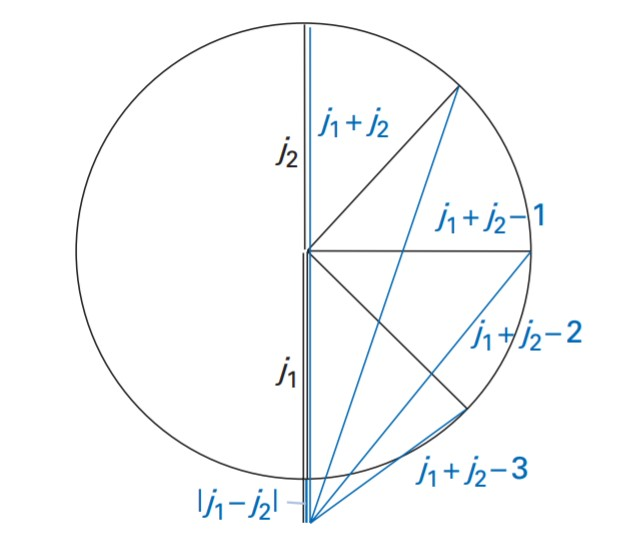
\includegraphics[width=6cm]{cgseries}
	\centering
	\caption{The allowed values of $j$ are just the third side of the triangle.}
	\label{fig:cgseries}
\end{figure}
\subsubsection{Relation between coupling schemes}
In \Cref{angmomcoup} we have introduced two pictures of coupling, the uncoupled 
and the coupled picture. Just as a recap, the uncoupled picture specifies the 
individual quantum numbers $j_i$ and $m_{ji}$. We usually use the \textbf{vector 
model of coupled angular momenta} to represent the differences between the two 
schemes, as in \Cref{fig:coupling}.
\begin{figure}[H]
	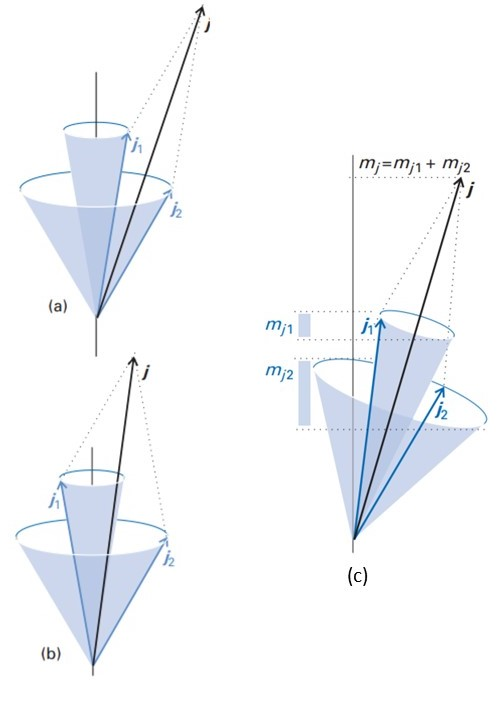
\includegraphics[width=6cm]{coupling}
	\centering
	\caption{(a) and (b) represent the uncoupled picture, in which we can't specify 
	$j_i$'s and $j$ simultaneously but can do so with $m_j$, as the $z$-component 
	is specified. (c) represents the coupled picture where the two $j_i$'s are 
	locked together, so $j$ (hence also $m_j$) is specified, but not the individual 
	components that add up to $m_j$.}
	\label{fig:coupling}
\end{figure}
We are more interested in the coupled picture as it gives us more immediate 
information of the system total parameters, as we shall see in 
\Cref{acc_for_spin}. So we should develop a way to quickly transform between the 
two pictures: the state $|j_1j_2;jm_j\rgl$ is built from a linear combination of 
all states with $m_{j1}+m_{j2}=m_j$:
\begin{equation}
\label{cgcoeffdef}
|j_1j_2;jm_j\rgl=\sum_{m_{j1},m_{j2}}C(m_{j1},m_{j2})|j_1m_{j_1};j_2m_{j2}\rgl,
\end{equation}
where the coefficients $C(m_{j1},m_{j2})$ are called \textbf{Clebsch-Gordan 
coefficients}, or vector coupling coefficients. For our case, $m_{j1}=m_{j2}=1/2$, 
the coefficients are easily seen to agree with our earlier efforts at establishing 
the singlet and triplet states. Omitting $j_1j_2$ in the notation and simply writing $|j,m_j\rgl$ or more specifically, $|S,M_S\rgl$, we have
\begin{equation}
\begin{aligned}
&|1,+1\rgl=\alpha_1\alpha_2\\
&|1,0\rgl=\frac{1}{\sqrt{2}}\alpha_1\beta_2+\frac{1}{\sqrt{2}}\beta_1\alpha_2\\
&|1,-1\rgl=\beta_1\beta_2\\
&|0,0\rgl=\frac{1}{\sqrt{2}}\alpha_1\beta_2-\frac{1}{\sqrt{2}}\beta_1\alpha_2. 
\end{aligned}
\end{equation}
The Clebsch-Gordan coefficients can be calculated as overlap integrals between 
the coupled and uncoupled states. We do so by right-multiplying \Cref{cgcoeffdef} 
by $\lgl j_1m'_{j1};j_2m'_{j2}|$:
\begin{equation}
\lgl j_1m'_{j1};j_2m'_{j2}|j_1j_2;jm_j\rgl=C(m'_{j1},m'_{j2}), 
\end{equation}
where other terms in the sum vanishes by the orthogonality of the states. This 
can be intuitively understood as how much the coupled state resembles the 
uncoupled state, or `how much' of the uncoupled state should be in the linear 
combination. For example, the state $|1,+1\rgl$ must be composed of $\alpha_1\alpha_2$ only as this is the only state with $M_S=+1$. 
\subsubsection{Atomic term symbols}
\label{term_symbols}
\hl{read chap 7 of atkins, and section on spin in B field in griffiths, priority: high. After that, re-write this section}
Term symbols give better descriptions than electron configurations, as we will see, same electronic configuration will give rise to different energies as a 
result of electrostatic interactions. The idea is to determine the total orbital 
angular momentum $\bvec{L}$ and the total spin angular momentum $\bvec{S}$ and 
then adding them vectorially to get the total angular momentum $\bvec{J}$:
\begin{equation}
\bvec{J}=\bvec{L}+\bvec{S}=\sum_i l_i+\sum_j s_j.
\end{equation}
This is called the \textbf{Russell-Saunders coupling} or \textbf{LS coupling}, 
which is only predominant in lighter ($Z<30$) atoms. \hl{same as spin-orbit coupling?}
The result of this sum is summarised as a \textbf{term symbol}, like
\begin{equation}
^{2S+1}L_J,
\end{equation}
where $L,S,J$ are the total orbital/total spin/total angular momentum quantum numbers, and $2S+1$ is known as the spin multiplicity. \\
With an argument exactly like the one given in \Cref{perm_totmom}, we can show 
that $\bvec{J}$ and $\bvec{S}$ are angular momenta and their values must run 
through integers and/or half integers. And since individual orbital angular 
momenta must be integers and individual spins can be both, so do the total. 
And another argument as in \Cref{perm_totmom} will give us that $J$ runs from 
$L+S$ to $|L-S|$. To summarise, the allowed values for the quantum numbers 
involved in the term symbol are
\begin{prt}[Term symbol]
The term symbol is
\begin{equation}
^{2S+1}L_J,
\end{equation}
where the allowed values are
\begin{equation}
\begin{aligned}
&S=0,1/2,1,3/2,\cdots\\
&(2S+1)=1,2,3,4,\cdots\\
&L=0,1,2,3,\cdots\\
&J=L+S,L+S-1,\cdots,|L-S|.
\end{aligned}
\end{equation}
\end{prt}
In analogy to assigning $s,p,d,f,\cdots$ to $\ell=0,1,2,3,\cdots$, we assign
$S,P,D,F,\cdots$ for $L=0,1,2,3,\cdots$. \\
Recall that the $z$-components of angular momenta simply add, \ie
\begin{equation}
\begin{aligned}
&L_z=\sum_i l_{zi}=\sum_i m_{li}=M_L\\
&S_z=\sum_i s_{zi}=\sum_i m_{si}=M_S
\end{aligned}
\end{equation}
The $M_S$ quantum number gives rise the $2S+1$ multiplicity (their energy will only be further split into levels in presence of external field \hl{todo: read up relevant stuff, reference, priority: low}). We will now look at a few examples. \\
\ \\
\textbf{Example 1: $ns^2$}
\begin{itemize}
	\item $s$ orbital means $\ell=0$, so $m_{li}=0$, and $M_L=0$, and this being the only allowed value of $M_L$ means $L=0$ or the S-state.
	\item The two spins must be antiparallel, so $M_S$ is also equal $0$, and so similarly $S=0$.
	\item By the same token, $J$ can also only be $0$.
	\item Therefore, the term symbol for $ns^2$ is $^1S_0$.
\end{itemize}
\textbf{Example 2: $np^6$}
\begin{itemize}
	\item $p$ orbital means $\ell=1$, so $m_{li}=-1,0,1$ so $M_L$ being the sum of all occupied orbitals (which is all of them) is $0$.
	\item Spins also all pair up to give $M_S=0$.
	\item Therefore $J$ can only be $0$
	\item The term symbol for $np^6$, and actually for \textbf{all} fully filled orbitals subshells, is $^1S_0$. It's also called \textbf{singlet S zero}.
\end{itemize}
\textbf{Example 3: }$ns^1n's^1$ (first excited state of Helium)
\begin{itemize}
	\item $M_L$ can only be zero as $m_{li}=0$.
	\item However now the spins are not confined to have antiparallel spins, and can independently take on values of $\pm1/2$, so $M_S$ can be $-1,0,1$. This means the largest value of $S$ is $1$ since that's the largest value $M_S$ can take on. So we must have $S=0,1$, corresponding to $^3S$ (triplet) and $^1S$ (singlet) states.
\end{itemize}
We list the possible states below:
\begin{center}
\begin{tabular}{c|c c c}
&\multicolumn{3}{c}{$M_S$}\\
$M_L$&$1$&$0$&$-1$\\
\hline
$0$&$0^+,0^+$&$0^+,0^-;0^-,0^+$&$0^-,0^-$
\end{tabular}
\end{center}
where $0^+$ means $m_l=0$ and $m_s=+1/2$ and vice versa. The middle two states are 
not indistinguishable because the spatial orbitals are not the same ($1s$ and 
$2s$)There are $4$ \textbf{microstates}. The triplet state accounts for one state 
from each column, and the singlet state must claim the remaining $M_S$ state, and 
it doesn't matter which one each state takes. \par
And we are left with $J$ to determine. We add $M_L$ and $M_S$ to get $M_J$. 
For the triplet state $M_J$, $M_J=1,0,-1$, so $J=1$. For the singlet state 
similarly $J=0$.\par
Therefore the two term symbols the configuration $ns^1n's^1$ correspond to are $^3S_1$ and $^1S_0$. \\
\ \\
\textbf{Example 4: }Carbon atom\\
\ \\
As shown previously, we do not need to worry about fully filled subshells and only need to focus on $2p^2$. Let's derive a general result first: 
\begin{lemma}[Number of electron assignments]
For $G$ number of \textbf{equivalent} (same subshell) spin-orbitals and $N$ 
electrons, which are indistinguishable, the number of ways to 
assign the electrons, $D(G,N)$ is 
\begin{equation}
D(G,N)=\frac{G!}{N!(G-N)!}.
\end{equation}
\end{lemma}
So for carbon, we have $15$ ways to assign the electrons. Intuitively, the first electron can take any of the $6$ spin-orbitals, the second can take the remaining 
$5$, and a factor of $2!$ is divided through for they are indistinguishable, 
giving a total of $15$ ways to arrange. \par
To find all these $15$ microstates we again use a table. But before that we need 
to find out the values of $M_L$ and $M_S$. It's easily seen that $M_L$ runs from 
$-2$ to $+2$ and $M_S$ from $-1$ to $+1$. So $L=0,1,2$ and $S=0,1$. The table is then 
\begin{center}
\begin{tabular}{c|c c c}
&\multicolumn{3}{c}{$M_S$}\\
$M_L$&$1$&$0$&$-1$\\
\hline
$2$&\highlight{1^+,1^+}&$1^+,1^-$&\highlight{1^-,1^-}\\
$1$&$0^+,1^+$&$1^+,0^-;1^-,0^+$&$0^-,1^-$\\
$0$&\highlight{0^+,0^+}$;1^+,-1^+$&$1^+,-1^-;-1^+,1^-;0^+,0^-$&$1^-,-1^-;$\highlight{0^-,0^-}\\
$-1$&$0^+,-1^+$&$0^+,-1^-;0^-,-1^+$&$0^-,-1^-$\\
$-2$&\highlight{-1^+,-1^+}&$-1^+,-1^-$&\highlight{-1^-,-1^-}
\end{tabular}
\end{center}
where we make no distinction like the previous case between $1^+,0^-$ and 
$0^-,1^+$ because the spatial orbitals are equivalent now. The grey terms are 
forbidden by the Pauli exclusion principle. We now assign term symbols to the 
microstates. \par
We start by remarking that although the \textbf{allowed} values of 
$L$ and $S$ is $0$ to $2$ and $0$ to $1$ respectively, the actual \textbf{permitted} term symbols are not necessarily all possible permutations of these values. For example, the largest value of $M_L$ is $2$ and it only occurs with $M_S=0$, this means that $L=2$ state only occurs with $S=0$. For the remaining states, the largest $M_L=1$, and it occurs with all three $M_S$ values, hence there must be a state with $L=1$ and $S=1$. We list the term symbols below:
\begin{itemize}
	\item $L=2$, $S=0$, \ie $^1D$: one state per row in the $M_S=0$ column. $J$ can only take up one value, which is $2$. The complete term symbol is $^1D_2$.
	\item $L=1$, $S=1$, \ie $^1P$: nine states per remaining cells. $J$ can take up values from $2$ to $0$, so complete term symbols are $^3P_2$, $^3P_1$, and $^3P_0$.\footnote{Another way to look at this is that the nine states correspond to $M_J$ of $2,1,1,0,0,-1,0,-1,-2$, so we can isolate three sets of $M_J$ running from $-J$ to $J$ with $J=0,1,2$ respectively.}
	\item $L=0$, $S=0$, term symbol $^1S_0$, naturally.
\end{itemize}
As can be seen, we don't really have to specify $J$ as it can be deduced from $S$ and $L$. The degeneracies of each state is given by $2J+1$. \par
At last, we can introduce Hund's rules, \hl{todo: theoretical foundations, priority: medium}:
\begin{thrm}[Hund's rules]
The three Hund's rules state that
\begin{enumerate}
	\item The state with the largest value of $S$ is the most stable (has the lowest energy), and stability decreases with decreasing $S$. 
	\item For states with the same value of $S$, the state with the largest value of $L$ is the most stable. 
	\item If the states have the same value of $L$ and $S$, then, for a subshell that is less than half filled, the state with the smallest value of $J$ is the most stable; for a subshell that is more than half filled, the state with the largest value of $J$ is the most stable. 
\end{enumerate}
\end{thrm}
\subsubsection{Molecular term symbols}
The following discussion only strictly applies to homonuclear diatomics, for which only the orbital angular momentum along the internucalear axis is defined.\par
The molecular term symbol is given in the form of 
\begin{equation}
	^{2\Sigma+1}\Lambda^{\pm}_{g/u},
\end{equation}
$\Sigma$ is just the spin angular momentum, effectively the half the number of unpaired electrons in the molecule.\par
$\Lambda$ is the orbital angular momentum \emph{along the internuclear axis}, given as
\begin{equation}
	\Lambda=\sum_i M_{L,i},
\end{equation}
with \emph{unpaired} electrons in $\sigma$ orbitals having $M_L=0$ and those in $\pi$ orbitals having $M_L=1$ and so on.\par
The $g/u$ labels denotes the \emph{inversion symmetry}, where the overall inversion symmetry is a direct product of the inversion symmetry of all occupied orbitals, with 
\begin{equation}
	g\times g=g\ \ u\times u=g\ \ g\times u=u\ \ u\times g=u.
\end{equation}
And finally the $\pm$ label denotes the \emph{mirror-plane} symmtry, where the mirror plane contains the internuclear axis, where $+$ means unchanged upon reflection and $-$ means the sign changes upon reflection. 
Mathematically speaking, reflection changes the sign of $\phi$. Let's see this in action\hl{draw diagram}, say we have the ground state of oxygen, which has an electronic configuration of $\pi^2$, which has two orbitals with $M_L=\pm 1$, which leads to two $^1\Delta$ states with two electrons in either orbitals, and a $^3\Sigma$ and $^1\Sigma$ state with two electrons in both states but two orientations. The wavefunctions for the two orbitals are
\begin{equation}
\begin{aligned}
	\pi_+&=F(\bvec{r_a},\bvec{r_b})e^{i\phi}\\
	\pi_-&=F(\bvec{r_a},\bvec{r_b})e^{-i\phi}
\end{aligned}
\end{equation}
we further define the reflection operator
\begin{equation}
	\sigma_{xy}\pi_{\pm}=\pi_{\mp}
\end{equation}
and the total wavefunction for the two electrons
\begin{equation}
	\Psi(\bvec{r_1},\bvec{r_2})=\frac{1}{\sqrt{2}}[\pi_+(1)\pi_-(2)\mp\pi_-(1)\pi_+(2)]\times\bvec{\sigma}_{\pm}
\end{equation}
where the top sign denotes triplet, whose spin wavefunction is symmetric to exchange, and the bottom sign denotes singlet. Now the action of the total reflection operator $\sigma_{\text{tot}}=\sigma_{xy}(1)\sigma_{xy}(2)$ is
\begin{equation}
\begin{aligned}
	\sigma_{\text{tot}}\Psi(\bvec{r_1},\bvec{r_2})&=\frac{1}{\sqrt{2}}\sigma_{xy}(1)\sigma_{xy}(2)[\pi_+(1)\pi_-(2)\mp\pi_-(1)\pi_+(2)]\times\bvec{\sigma}_{\pm}\\
	&=\frac{1}{\sqrt{2}}[\pi_-(1)\pi_+(2)\mp\pi_+(1)\pi_-(2)]\times\bvec{\sigma}_{\pm}\\
	&=\mp\Psi(\bvec{r_1},\bvec{r_2})
\end{aligned}
\end{equation}
therefore we see that the final full term symbols are $^3\Sigma^-$ and $^1\Sigma^+$. \par
This is only going to matter in $\Lambda=0$ ($\Sigma$) states, this is because all other states have a two-fold degeneracy, so the reflection operation is just going to interchange them, whereas in $\Sigma$ states there's no degeneracy.\par
\textbf{More exmamples}\par
$1\sigma^1\ 2\sigma^1$\\
As the electrons don't occupy the same orbitals, Pauli exclusion principle doesn't apply anyway, and also, since $\sigma$ MOs have no $\phi$ dependence, it has to be unchanged upon reflection, therefore $^1\Sigma^+$ and $^3\Sigma^+$ are produced.\par
$\sigma^1$\\
Similar argument produces $^2\Sigma^+$.\par
Closed shell\\
Close shells must have $S=0$ which forces the singlet configuration, which means antisymmetric spin wavefunction and hence $^1\Sigma^+$.\par
$\pi^1$\\
This simply produces $^2\Pi$, specifying the signs is unnecessary as the term is 2-degenerate anyway.

\section{Identical particles}
\subsection{Two particle systems}
\subsubsection{The \sch}
The state of a two-particle system is a function of both particle's coordinates 
and time:
\begin{equation}
\ups(\bvec{r_1},\bvec{r_2},t).
\end{equation}
Its time evolution is, as always, determined by the \sch
\begin{equation}
i\hbar\diffp{\ups}{t}=H\ups, 
\end{equation}
where the Hamiltonian is 
\begin{equation}
H=-\frac{\hbar^2}{2m_1}\onabla_1^2-\frac{\hbar^2}{2m_2}\onabla_2^2+V(\bvec{r_1},\bvec{r_2},t)
\end{equation}
The probability of finding particle $1$ in $d^3\bvec{r_1}$ and 
particle $2$ in $d^3\bvec{r_2}$ is
\begin{equation}
|\ups(\bvec{r_1},\bvec{r_2},t)|^2d^3\bvec{r_1}d^3\bvec{r_2}. 
\end{equation}
The normalisation requirement is therefore
\begin{equation}
\int|\ups(\bvec{r_1},\bvec{r_2},t)|^2d^3\bvec{r_1}d^3\bvec{r_2}=1.
\end{equation}
For \textbf{time-independent} potentials, we can use the usual separation of 
variables:
\begin{equation}
\ups(\bvec{r_1},\bvec{r_2},t)=\psi(\bvec{r_1},\bvec{r_2})e^{-iEt/\hbar}, 
\end{equation}
where $\psi$ is such that
\begin{equation}
H\psi=E\psi.
\end{equation}
\subsubsection{Centre-of-mass coordinates}
If, in a \textbf{two particle system}, where the potential depends only on 
$\bvec{r}\equiv\bvec{r_1}-\bvec{r_2}$ between the two particles, we can use the 
centre-of-mass coordinates to simplify and \textit{separate} the \sch as follows: 
we define the \textbf{centre-of-mass coordinate}:
\begin{equation}
\bvec{R}\equiv\frac{m_1\bvec{r_1}+m_2\bvec{r_2}}{m_1+m_2}
\end{equation}
Now, we need to re-write the \sch in terms of the new coordinates, 
and first of all we need to write out the Hamiltonians, which is fiddly to do: 
we first need to see that 
\begin{equation}
\onabla_1f=\diffp{f}{r_{1_x}}+\diffp{f}{r_{1_y}}+\diffp{f}{r_{1_z}}.
\end{equation}
So to re-write it, we note that $r_{1_x}$ is only dependent on $r_x$ and $R_x$, 
and so on, so
\begin{equation}
\label{fr1x}
\begin{aligned}
\diffp{f}{r_{1_x}}&=\diffp{f}{r_x}\diffp{r_x}{r_{1_x}}+\diffp{f}{R_x}\diffp{R_x}{r_{1_x}}\\
&=\diffp{f}{r_x}+\diffp{f}{R_x}\frac{\mu}{m_2}, 
\end{aligned}
\end{equation}
and
\begin{equation}
\begin{aligned}
\diffp{f}{r_{2_x}}&=\diffp{f}{r_x}\diffp{r_x}{r_{2_x}}+\diffp{f}{R_x}\diffp{R_x}{r_{2_x}}\\
&=-\diffp{f}{r_x}+\diffp{f}{R_x}\frac{\mu}{m_1}, 
\end{aligned}
\end{equation}
and so on for other components, so
\begin{subequations}
\begin{align}
&\onabla_1=\onabla_r+\frac{\mu}{m_2}\onabla_R\\
&\onabla_2=-\onabla_r+\frac{\mu}{m_1}\onabla_R.
\end{align}
\end{subequations}
To get the Laplacian, we note that it's not equivalent to left multiplying 
the transformed nabla operator twice, but instead we have to go 
back to \Cref{fr1x}, and differentiating it again wrt $r_{1_x}$ and so on:
\begin{equation}
\begin{aligned}
\diffp[2]{f}{r_{1_x}}&=\lf(-\diffp{}{r_x}+\frac{\mu}{m_2}\diffp{}{R_x}\rt)\lf(-\diffp{f}{r_x}+\diffp{f}{R_x}\frac{\mu}{m_2}\rt)\\
&=\diffp[2]{f}{r_x}-\diffp{f}{r_x,R_x}\frac{2\mu}{m_2}+\diffp[2]{f}{R_x}\lf(\frac{\mu}{m_2}\rt)^2,
\end{aligned}
\end{equation}
and 
\begin{equation}
\begin{aligned}
\diffp[2]{f}{r_{2_x}}&=\lf(\diffp{}{r_x}+\frac{\mu}{m_1}\diffp{}{R_x}\rt)\lf(\diffp{f}{r_x}+\diffp{f}{R_x}\frac{\mu}{m_1}\rt)\\
&=\diffp[2]{f}{r_x}-\diffp{f}{r_x,R_x}\frac{2\mu}{m_1}+\diffp[2]{f}{R_x}\lf(\frac{\mu}{m_1}\rt)^2,
\end{aligned}
\end{equation}
so we have
\begin{equation}
-\frac{\hbar^2}{2m_1}\onabla^2_1=-\frac{\hbar^2}{2m_1}\onabla_r^2-\onabla^2_R\frac{\hbar^2\mu^2}{m_1m_2^2}-(\text{mixed partial term})
\end{equation}
and 
\begin{equation}
-\frac{\hbar^2}{2m_1}\onabla^2_2=-\frac{\hbar^2}{2m_2}\onabla_r^2-\onabla^2_R\frac{\hbar^2\mu^2}{m_2m_1^2}+(\text{same mixed partial term}).
\end{equation}
Finally, the \sch is 
\begin{equation}
\lf[-\frac{\hbar^2}{2(m_1+m_2)}\onabla^2_R-\frac{\hbar^2}{2\mu}\onabla^2_r+V(\bvec{r})\rt]\psi=E\psi. 
\end{equation}
We attempt separation of variables:
\begin{equation}
\psi(\bvec{R},\bvec{r})=\psi_R(\bvec{R})\psi_r(\bvec{r}),
\end{equation}
and we obtain two equations:
\begin{subequations}
\begin{align}
-\frac{\hbar^2}{2(m_1+m_2)}\onabla^2_R\psi_R&=E_R\psi_R\\
\lf[-\frac{\hbar^2}{2\mu}\onabla_r^2+V(\bvec{r})\rt]\psi_r&=E_r\psi_r.
\end{align}
\end{subequations}
This is saying that we have successfully decoupled the equation into two 
independent systems: the total mass ($m_1+m_2$), moving as a 
free particle ($0$ potential) and the relative motion as a 
single particle with reduced mass subject to potential $V$. 
\subsubsection{Bosons and fermions}
Suppose we now have a two particle system that is non-interacting, which is to 
say that the two particles are in their own one-particle states and that they 
are independent - this is by no means always true, as in the singlet spin 
configuration where two spins are correlated - we can write
\begin{equation}
\psi(\bvec{r}_1,\bvec{r}_2)=\psi_a(\bvec{r}_1)\psi_b(\bvec{r}_2).
\end{equation}
In writing this we have presumed that the two particles are 
\textbf{distinguishable}, otherwise the labels $a$ and $b$ wouldn't make any 
sense. However, almost all the particles we will be dealing with will 
\textit{not} be distinguishable. Therefore, the most we can say its that 
\textit{one} particle is in state $a$ and the other in state $b$. 
We note that since they are insdistinguishable, the exchange of labels 
\textit{must} have no effect on the probability density, \ie
\begin{equation}
|\psi(1,2)|^2=|\psi(2,1)|^2,\ \imp\ \psi(1,2)=\pm\psi(2,1).
\end{equation}
So this means we can write
\begin{equation}
\psi_{\pm}(\bvec{r}_1,\bvec{r}_2)=A[\psi_a(\bvec{r}_1)\psi_b(\bvec{r}_2)\pm\psi_b(\bvec{r}_1)\psi_a(\bvec{r}_2)]. 
\end{equation}
This wavefunction is \textit{non-committal} as to which particle is in which 
state, but when do we use which sign? We introduce the postulate
\begin{post}[Bosons and fermions]
\ \\
All particles with \textit{integer} spins are bosons, and\\
all particles with \textit{half integer} spins are fermions. \\
We use the \textit{plus sign} for bosons and \textit{minus sign} for fermions. 
\end{post}
It then follows that 
\begin{thrm}[Pauli exclusion principle]
Two identical fermions, for example, two electrons, cannot occupy the same state, 
for if $\psi_a=\psi_b$, then 
\begin{equation}
\psi_-(\bvec{r}_1,\bvec{r}_2)=A[\psi_a(\bvec{r}_1)\psi_a(\bvec{r}_2)-\psi_a(\bvec{r}_1)\psi_a(\bvec{r}_2)]=0,
\end{equation}
and we are left with no wavefunction at all. 
\end{thrm}
A more general re-formulation of problem requires the introduction of 
the \textbf{exchange operator}:
\begin{defi}[Exchange operator]
The exchange operators is defined as 
\begin{equation}
Pf(\bvec{r}_1,\bvec{r}_2)=f(\bvec{r}_2,\bvec{r}_1). 
\end{equation}
\end{defi}
\begin{defi}[Properties of the exchange operator]
\ \\
(1) It is immediately clear that
\begin{equation}
P^2=I.
\end{equation}
(2) And therefore the eigenvalues of $P$ are $\pm1$. \\
(3) If we have two \textit{identical} particles, the Hamiltonian must treat them the 
same way: $m_1=m_2$ and $V(\bvec{r}_1,\bvec{r}_2)=V(\bvec{r}_2,\bvec{r}_1)$, therefore $P$ and $H$ are compatible observables: 
\begin{equation}
[P,H]=0.
\end{equation}
\end{defi}
\begin{thrm}[Symmetrisation requirement]
\label{sym_req}
Because $P$ and $H$ commute, we can find simultaneous eigenstates of both, \ie 
we can find solutions to \sch that are either symmetric (eigenvalue $+1$) or 
antisymmetric (eigenvalue $-1$) under excahnge of labels:
\begin{equation}
\psi(\bvec{r}_1,\bvec{r}_2)=\pm\psi(\bvec{r}_2,\bvec{r}_1). 
\end{equation}
Therefore, if a system begins in a state it must remain in this state. 
The plus sign is for bosons and negative for fermions.
\end{thrm}
\subsubsection{Exchange forces}
We examine a 1D example. Let's suppose one particle is in $\psi_a(x)$ and another in $\psi_b(x)$, 
and these two states are orthogonal and normalised. \textit{If} the two particles 
are distinguishable, and number $1$ is the one in state $\psi_a$, then the 
composite wavefunction is 
\begin{equation}
\label{comp_dist}
\psi(x_1,x_2)=\psi_a(x_1)\psi_b(x_2).
\end{equation}
If they are identical bosons or fermions, the composite will be 
\begin{equation}
\label{comp_iden}
\psi_{\pm}(x_1,x_2)=\frac{1}{\sqrt{2}}[\psi_a(x_1)\psi_b(x_2)\pm\psi_b(x_1)\psi_a(x_2)].
\end{equation}
Let's calculate the expectation value of the square of the separation distance 
between the two particles, given by
\begin{equation}
\lgl (x_1-x_2)^2\rgl=\lgl x_1^2\rgl+\lgl x_2^2\rgl-2 \lgl x_1x_2\rgl. 
\end{equation}
\textbf{Case 1: Distinguishable particles}\\
We use the wavefunction in \Cref{comp_dist}:
\begin{equation}
\lgl x_1\rgl=\int x_1^2|\psi_a(x_1)|^2\dx_1\int|\psi_b(x_2)|^2\dx_2=\lgl x^2\rgl_a, 
\end{equation}
(the expectation of $x^2$ in the \textit{one-particle} state $\psi_a$) so similarly 
\begin{equation}
\lgl x_2^2\rgl=\lgl x_2^2\rgl_b. 
\end{equation}
And
\begin{equation}
\lgl x_1x_2\rgl=\int x_1|\psi_a(x_1)|^2\dx_1\int x_2|\psi_b(x_2)|^2\dx_2=\lgl x\rgl_a \lgl x\rgl_b.
\end{equation}
Collecting, we have
\begin{equation}
\label{delx_dist}
\lgl (x_1-x_2)^2\rgl=\lgl x^2\rgl_a+\lgl x^2\rgl_b-2 \lgl x\rgl_a \lgl x\rgl_b.
\end{equation}
\textbf{Case 2: Identical particles}\\
We now have to use the wavefunctions in \Cref{comp_iden}:
\begin{equation}
\begin{aligned}
\lgl x_1^2\rgl=&\frac{1}{2}\lf[\int x_1^2|\psi_a(x_1)|^2\dx_1\int|\psi_b(x_2)|^2\dx_2\rt.\\
&+\int x_1^2|\psi_b(x_1)|^2\dx_1\int|\psi_a(x_2)|^2\dx_2\\
&\pm\int x_1^2\psi_a(x_1)^*\psi_b(x_1)\dx_1\int\psi_b(x_2)^*\psi_a(x_2)\dx_2\\
&\lf.\pm \int x_1^2\psi_b(x_1)^*\psi_a(x_1)\dx_1\int\psi_a(x_2)^*\psi_b(x_2)\dx_2\rt]\\
=&\frac{1}{2}\lf[\lgl x^2\rgl_a+\lgl x^2\rgl_b\pm0\pm0 \rt]\\
=&\frac{1}{2}\lf(\lgl x^2\rgl_a+\lgl x^2\rgl_b\rt).
\end{aligned}
\end{equation}
And likewise
\begin{equation}
\lgl x_2^2\rgl=\frac{1}{2}\lf(\lgl x^2\rgl_b+\lgl x^2\rgl_a\rt).
\end{equation}
We observe that 
\begin{equation}
\lgl x_1^2\rgl=\lgl x_2^2\rgl
\end{equation}
since we can't tell them apart. Now
\begin{equation}
\begin{aligned}
\lgl x_1x_2\rgl=&\frac{1}{2}\lf[\int x_1|\psi_a(x_1)|^2\dx_1\int x_2|\psi_b(x_2)|^2\dx_2\rt.\\
&+\int x_1|\psi_b(x_1)|^2\dx_1\int x_2|\psi_a(x_2)|^2\dx_2\\
&\pm\int x_1\psi_a(x_1)^*\psi_b(x_1)\dx_1\int x_2\psi_b(x_2)^*\psi_a(x_2)\dx_2\\
&\lf.\pm\int x_1\psi_b(x_1)^*\psi_a(x_1)\dx_1\int x_2\psi_a(x_2)^*\psi_b(x_2)\dx_2 \rt]\\
=&\frac{1}{2}\lf(\lgl x\rgl_a \lgl x\rgl_b+\lgl x\rgl_b \lgl x\rgl_a\pm\lgl x\rgl_{ab} \lgl x\rgl_{ba}\pm \lgl x\rgl_{ba} \lgl x\rgl_{ab} \rt)\\
=&\lgl x\rgl_{a} \lgl x\rgl_{b}\pm|\lgl x\rgl_ab|^2, 
\end{aligned}
\end{equation}
where 
\begin{equation}
\lgl x\rgl_{ab}\equiv\int x\psi_a(x)^*\psi_b(x)\dx.
\end{equation}
Collecting we have
\begin{equation}
\label{delx_iden}
\lgl (x_1-x_2)^2\rgl_{\pm}=\lgl x^2\rgl_a+\lgl x^2\rgl_b-2 \lgl x\rgl_a \lgl x\rgl_b\mp2 |\lgl x\rgl_{ab}|^2.
\end{equation}
\begin{thrm}[Exchange force]
\ \\
By comparing \Cref{delx_dist} and \Cref{delx_iden}, we see that the difference 
lies in the final term:
\begin{equation}
\lgl (\Delta x)^2\rgl_{\pm}=\lgl (\Delta x)^2\rgl_d\mp2 |\lgl x\rgl_{ab}|^2,
\end{equation}
where the subscript $d$ stands for `distinguishable'. 
Therefore we can see that identical bosons are closer together and identical 
fermions further apart than distinguishable particles in the same two states. 
Notice that $\lgl x\rgl_{ab}$ \textbf{vanishes} unless the two wavefunctions 
\textbf{overlap}. Therefore, it is acceptable to treat electrons with 
non-overlapping wavefunctions as distinguishable. The increase or decrease 
in between identical particles are called an \textbf{exchange force}.
\end{thrm}
We now take a look at the hydrogen molecule, H$_2$. To a good approximation
\footnote{See next section.}, the ground state consists of one electron in the 
hydrogen atom ground state centred around nucleus $1$ and another around nucleus 
$2$. If electrons were bosons, the exchange force would concentrate the electrons 
towards the middle of the internuclear space, and as a result pull the protons 
inward, accounting for the covalent bond. However, electrons are fermions, and 
that would mean the concentration of negative charge should be on the wings, 
tearing the molecule apart. This is obviously wrong, and we are reminded that 
we have been ignoring spins all this while - the symmetrisation requirement 
(\Cref{sym_req}) requires that the \textbf{complete wavefunctions} of fermions be 
antisymmetric, not just the spatial wavefunctions. The complete wavefunctions of 
electrons are
\begin{equation}
\psi_e(\bvec{r},\bvec{s})=\psi(\bvec{r})\chi(\bvec{s}).
\end{equation}
This is assuming that the spin and the spatial wavefunction are 
\textit{uncoupled}, therefore separable. Under the same assumption, we can write 
the two-electron state as
\begin{equation}
\psi_{2e}(\bvec{r}_1,\bvec{r}_2,\bvec{s}_1,\bvec{s}_2)=\psi_{\pm}(\bvec{r}_1,\bvec{r}_2)\chi(\bvec{s}_1,\bvec{s}_2), 
\end{equation}
where $\chi(\bvec{s}_1,\bvec{s}_2)$ can be one of the four (three triplet one 
singlet) states in \Cref{add_moment}. Now, we must require bonding, therefore 
symmetric\footnote{Remember that the exchange force favours bonding as long as the 
\textit{spatial} wavefunction is symmetric, and it makes no use of the spinor as 
the `integration' of orthonormal spinors always return the Kronecker delta.}, \textit{spatial} wavefunctions. 
We remember that the singlet state is antisymmetric\footnote{We can actually 
derive this from symmetry requirements alone, stating from the four possible 
combinations and then consider their coefficients as in \cite{spincoeff}.}, therefore the spatial 
wavefunction of the electron that's multiplied to it can (and must) be symmetric. 
This can be confusing because we appear to have just derived that all 
electron wavefunctions must be antisymmetric. But in fact we have not, 
\Cref{sym_req} only requires that the complete wavefunction be accordingly 
symmetrised, not spatial or spinor parts separately. \par
Therefore, we have now shown that the bonding orbital will have electrons occupy 
the singlet configuration, with total spin zero, and the antibonding orbital one of the triplet configurations. \par
Another more elementary but more intuitive way to look at this is that electrons 
with the same spin cannot be found at the same spot and the electron density will be low around another electron with the same spin. This is not the case for electrons with opposite spin. Because of the Coulombic repulsion, electrons with like spins are lower in energy than those with opposite spin. This explains in part the Hund's rule. Also, the triplet state is more stable than the singlet state, however the latter is essential for chemical bonding to happen, and bonding happens because the lowering in energy more than compensates for the exchange force. 